\chapter{Тест2}

Тестовая глава для печати всех иллюстраций.

\newpage

%----------------------------------------------------------------
% 1 ГЛАВА
%----------------------------------------------------------------


\begin{figure}[h]
	\centering
	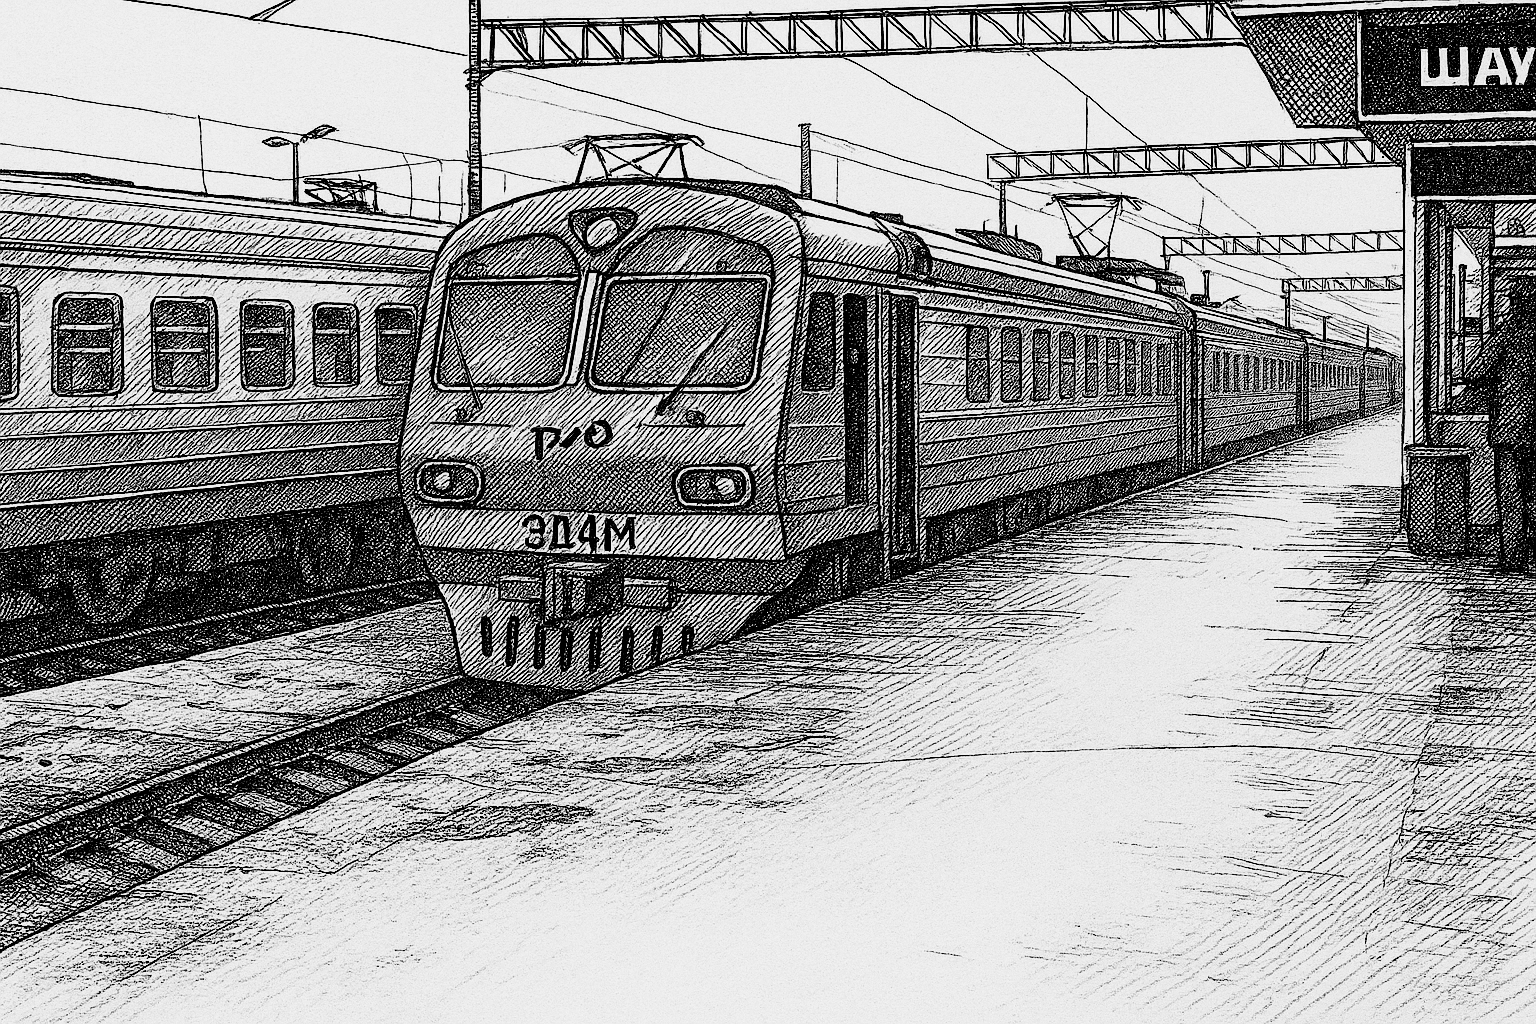
\includegraphics[width=1.0\textwidth]{01_train}
	\caption{\small\textit{...в электричке c Курского вокзала...}}	
\end{figure}

%----------------------------------------------------------------
% 2 ГЛАВА
%----------------------------------------------------------------

\newpage

Сеструха, тем временем, задорно отплясывала в центре зала, широко улыбаясь, светя забитой татухой рукой и~оголёнными плечами, справедливо упиваясь торжеством молодости, красоты, задора. Светлые завитые локоны подплясывали в такт движениям, вишнёвое вечернее платье подчёркивало все её сочные достоинства.

\noindent
\begin{minipage}{0.48\textwidth}
	\setlength{\parindent}{1.0cm}  % Включаем красную строку
	
	\indent \diagdash Пошли~потанцуем?\mdash вдруг жарко шепнула жена на~ухо Шурику.
	
	\indent \diagdash А пошли!\mdash он приобнял жену и закружил в толпе танцующих гостей, словно желая выкружить все крамольные мысли из~головы$\ldots$
	
	\indent $\ldots$Стол ломился, друзья широко, разгульно праздновали:
	
	\indent \diagdash Дорогие Кирилл и~Надежда$\ldots$\mdash полились речи, всё как обычно, ничего нового. От этих речей Шурику вдруг стало невообразимо скучно, да~так, что свело скулы.
\end{minipage}\hfill
\begin{minipage}{0.5\textwidth}
	\centering
	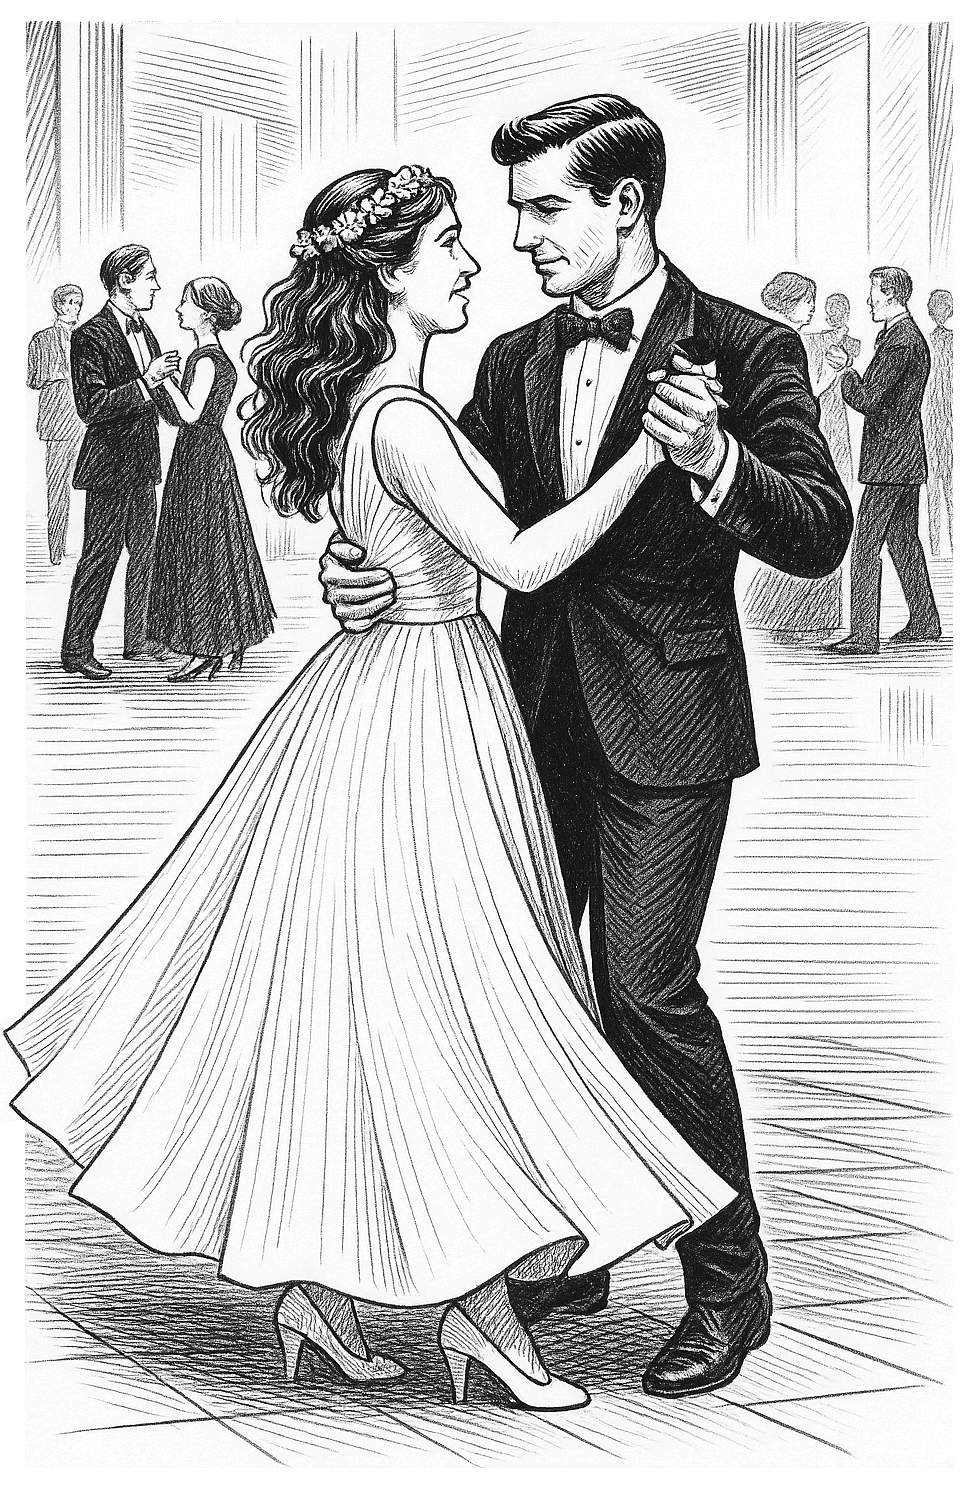
\includegraphics[width=\linewidth]{02_wedding}
	
	{\small\textit{...в платье белом...}}
\end{minipage}

%----------------------------------------------------------------
% 3 ГЛАВА
%----------------------------------------------------------------
\newpage

\begin{figure}[h]
	\centering
	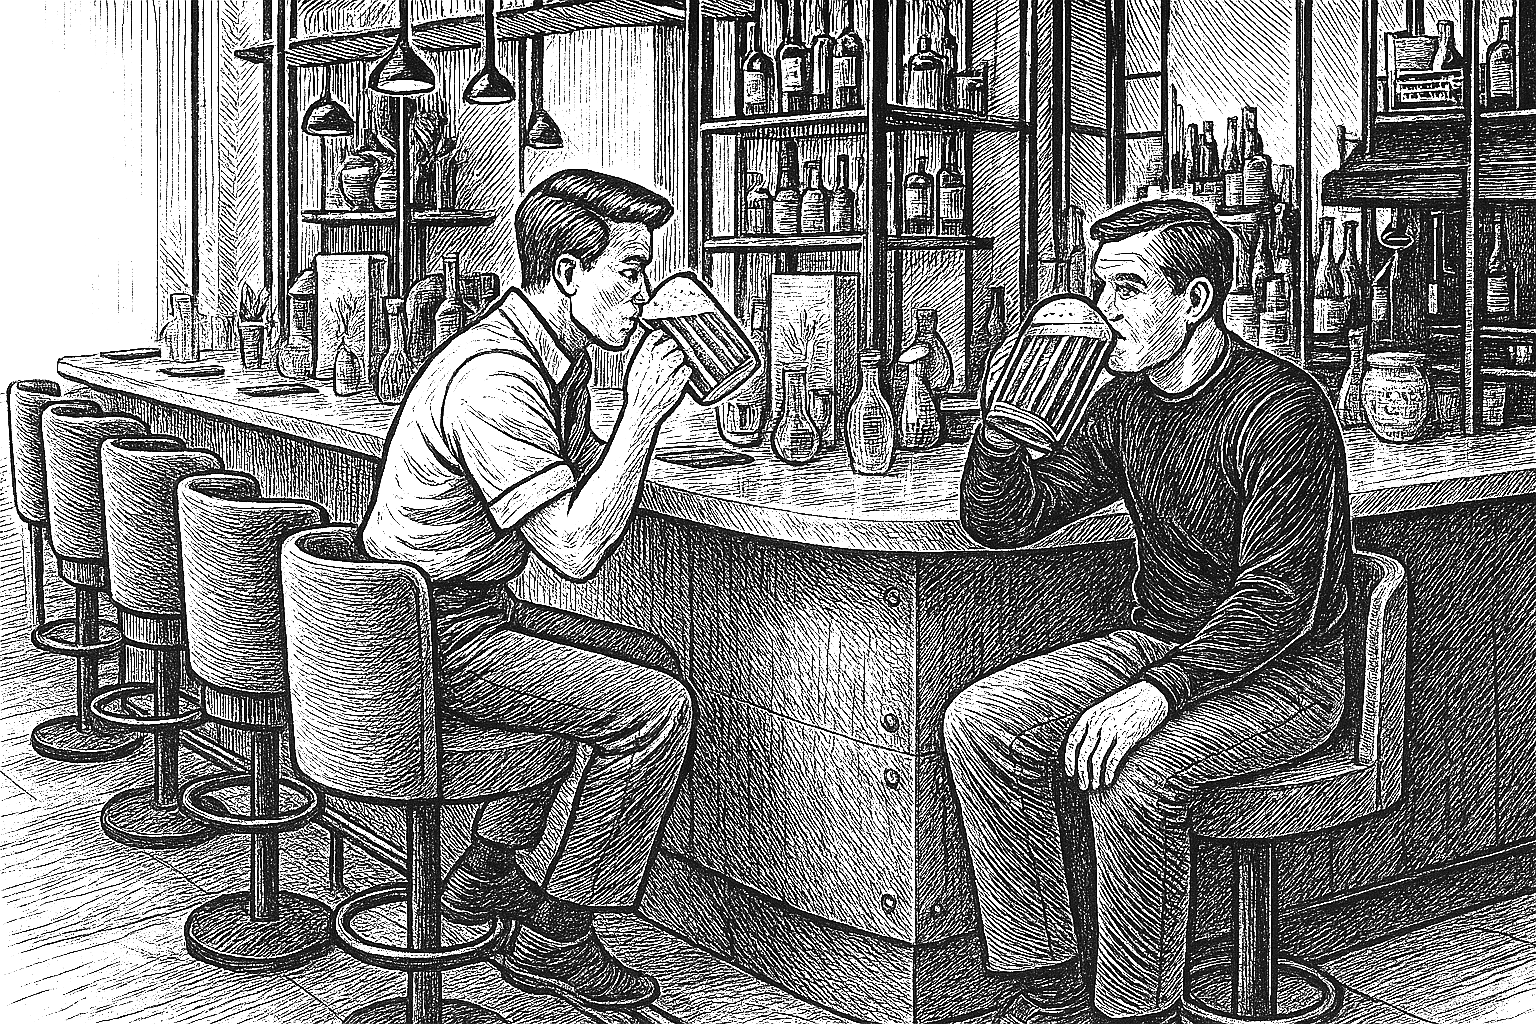
\includegraphics[width=1.0\textwidth]{03_1_beer}
	\caption{\small\textit{...Адмирал с Замполитом сидели в пивнушке...}}
\end{figure}

%----------------------------------------------------------------
\newpage

\noindent
\begin{minipage}{0.55\textwidth}
	\setlength{\parindent}{1.0cm}  % Включаем красную строку
	\setlength{\parskip}{0.25cm}     % Межабзацный отступ, как в основном тексте
	
	\noindent байдарочных фартука, надев их на себя. Узнал издалека, не~ошиблась.
	
	\diagdash Так, вот, держите,\mdash стала передавать, снимая с~себя снарягу, байдарочница, а~Шурик стал навешивать фартуки и~жилеты уже на~себя.
	
	\diagdash А остальное?	
	
	\diagdash А остальное на другом складе, надо пройти минут пять, пошли?\mdash маняще мотнула она головой в~сторону 9\sdash этажек и~поправила волосы$\ldots$
\end{minipage}\hfill
\begin{minipage}{0.40\textwidth}
	\centering
	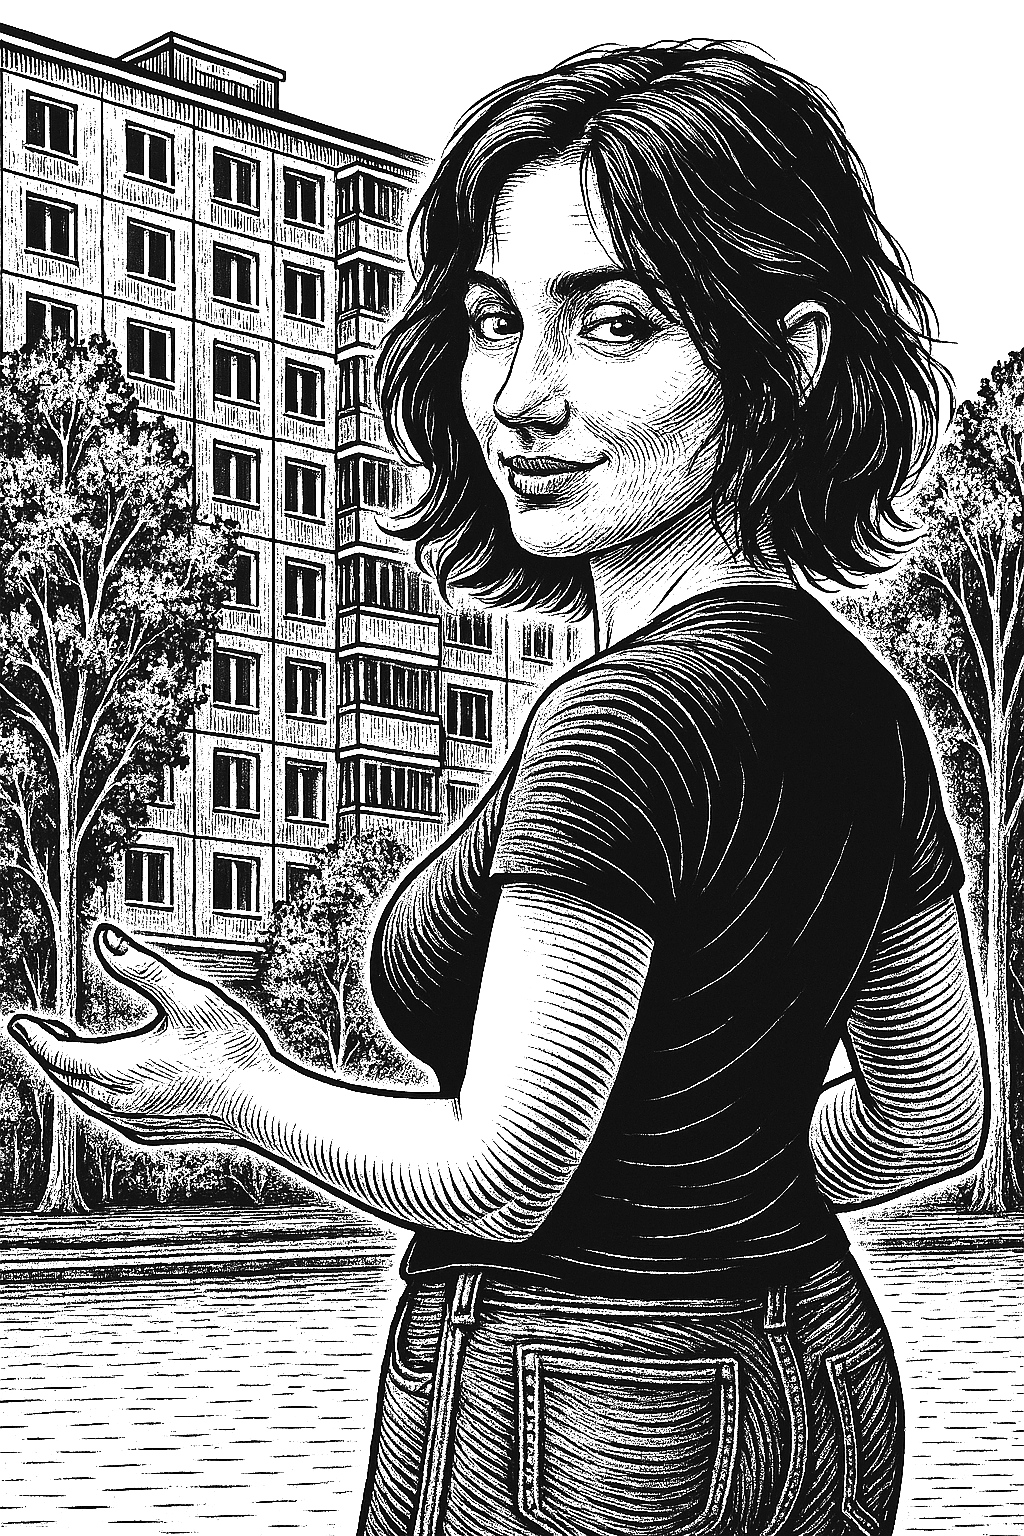
\includegraphics[width=\linewidth]{04_1_girl}
	
	{\small\textit{...с~хитрым~прищуром...}}
\end{minipage}

%----------------------------------------------------------------
\newpage

\begin{wrapfigure}[11]{l}{0.49\textwidth}
	%\begin{figure}[h]
	\centering
	%	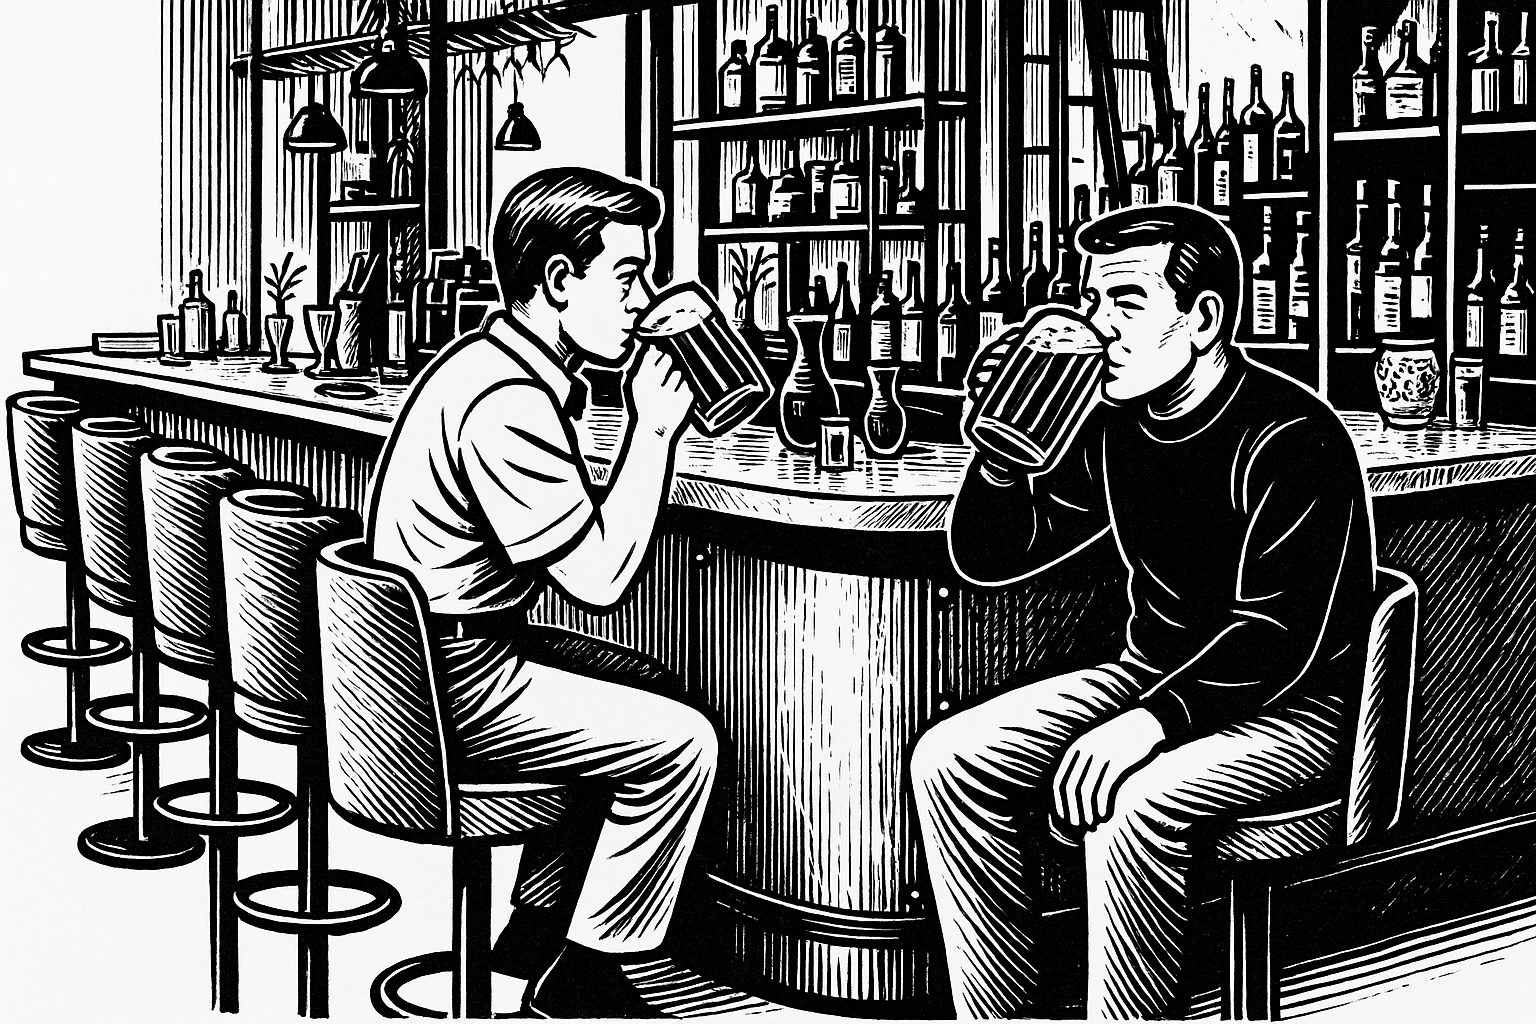
\includegraphics[width=1.0\textwidth]{3_new3}
	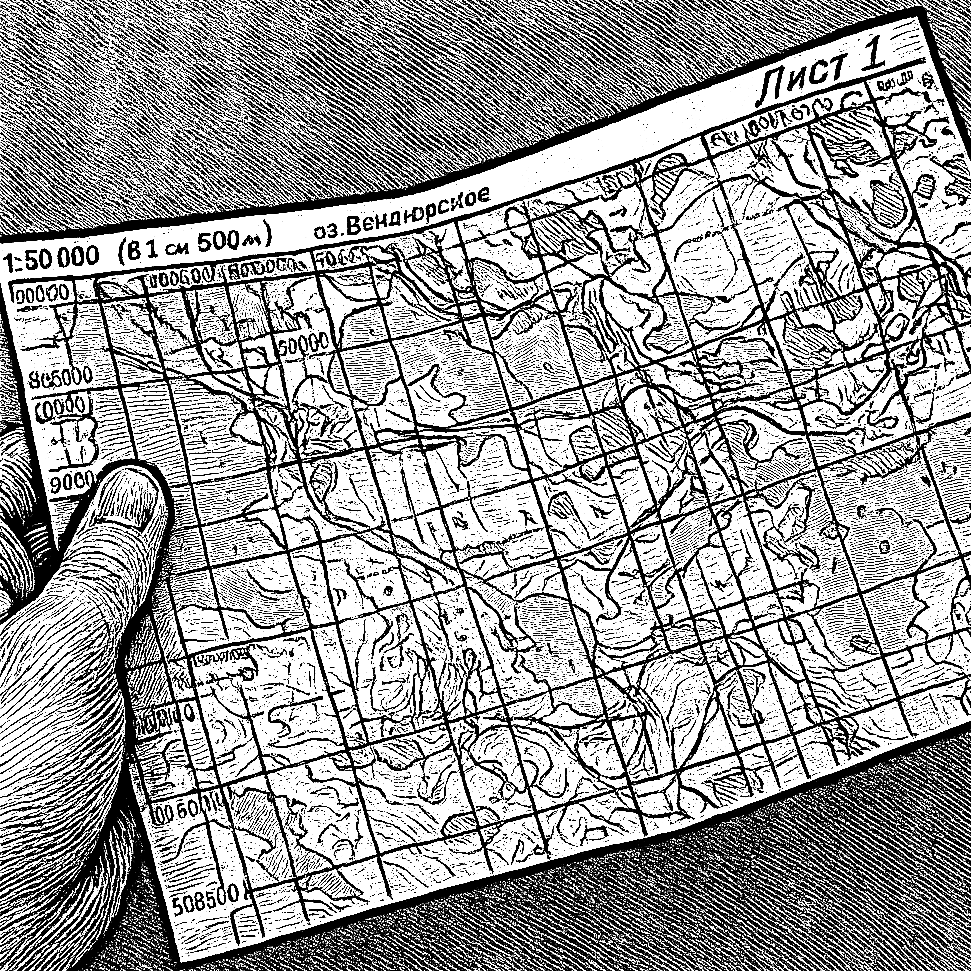
\includegraphics[width=0.47\textwidth]{05_1_map}
	\caption{\small\textit{...повело плёнку...}}
	%\end{figure}
\end{wrapfigure}

\diagdash А~дубликат~есть?\mdash заволновалась Надя.

\diagdash Нет уж, пойдём по такой карте.\mdash Замполит деланно закатил глаза.\mdash Потеряемся, как пить дать! Ё\sdash моё! Ну всё, Шурик, по~такой карте идти нельзя! 

\diagdash Всё пропало, Кирь!\mdash подыграл тот.


%----------------------------------------------------------------
% 4 ГЛАВА
%----------------------------------------------------------------

%\newpage
\vspace{20mm}

\begin{figure}[h]
	\centering
	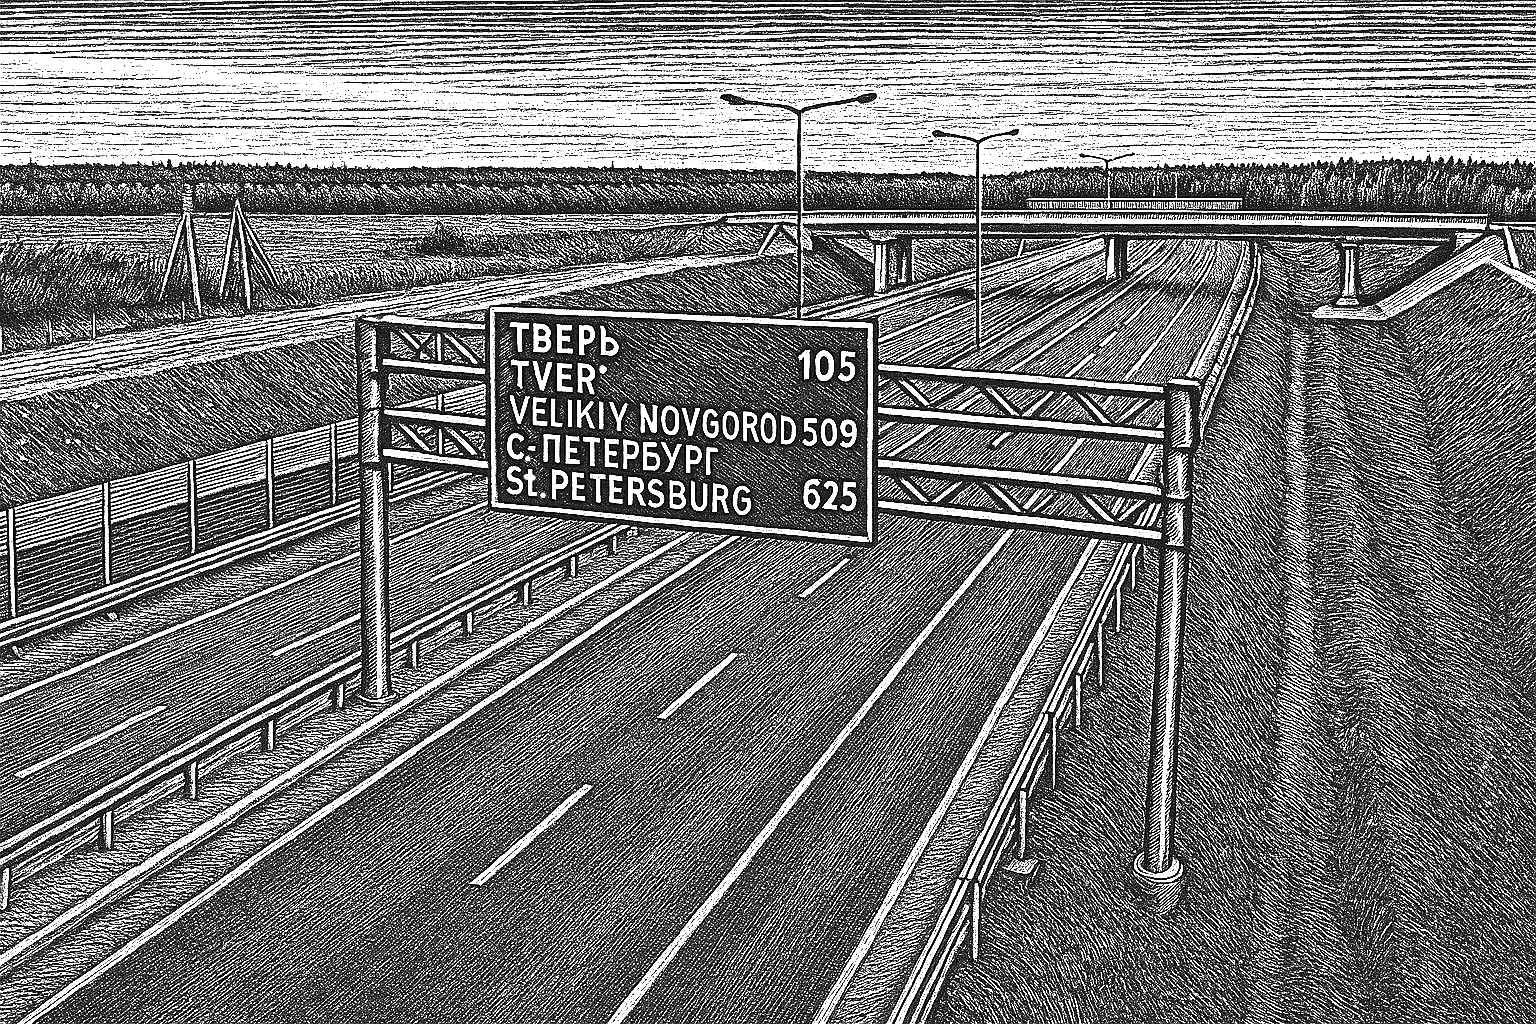
\includegraphics[width=1.0\textwidth]{06_1_highway}
	\caption{\small\textit{...бодро рванул вперёд по автостраде, утапливая педаль газа...}}
\end{figure}

%----------------------------------------------------------------
% 5 ГЛАВА
%----------------------------------------------------------------
\newpage

\begin{figure}[h]
	\centering
	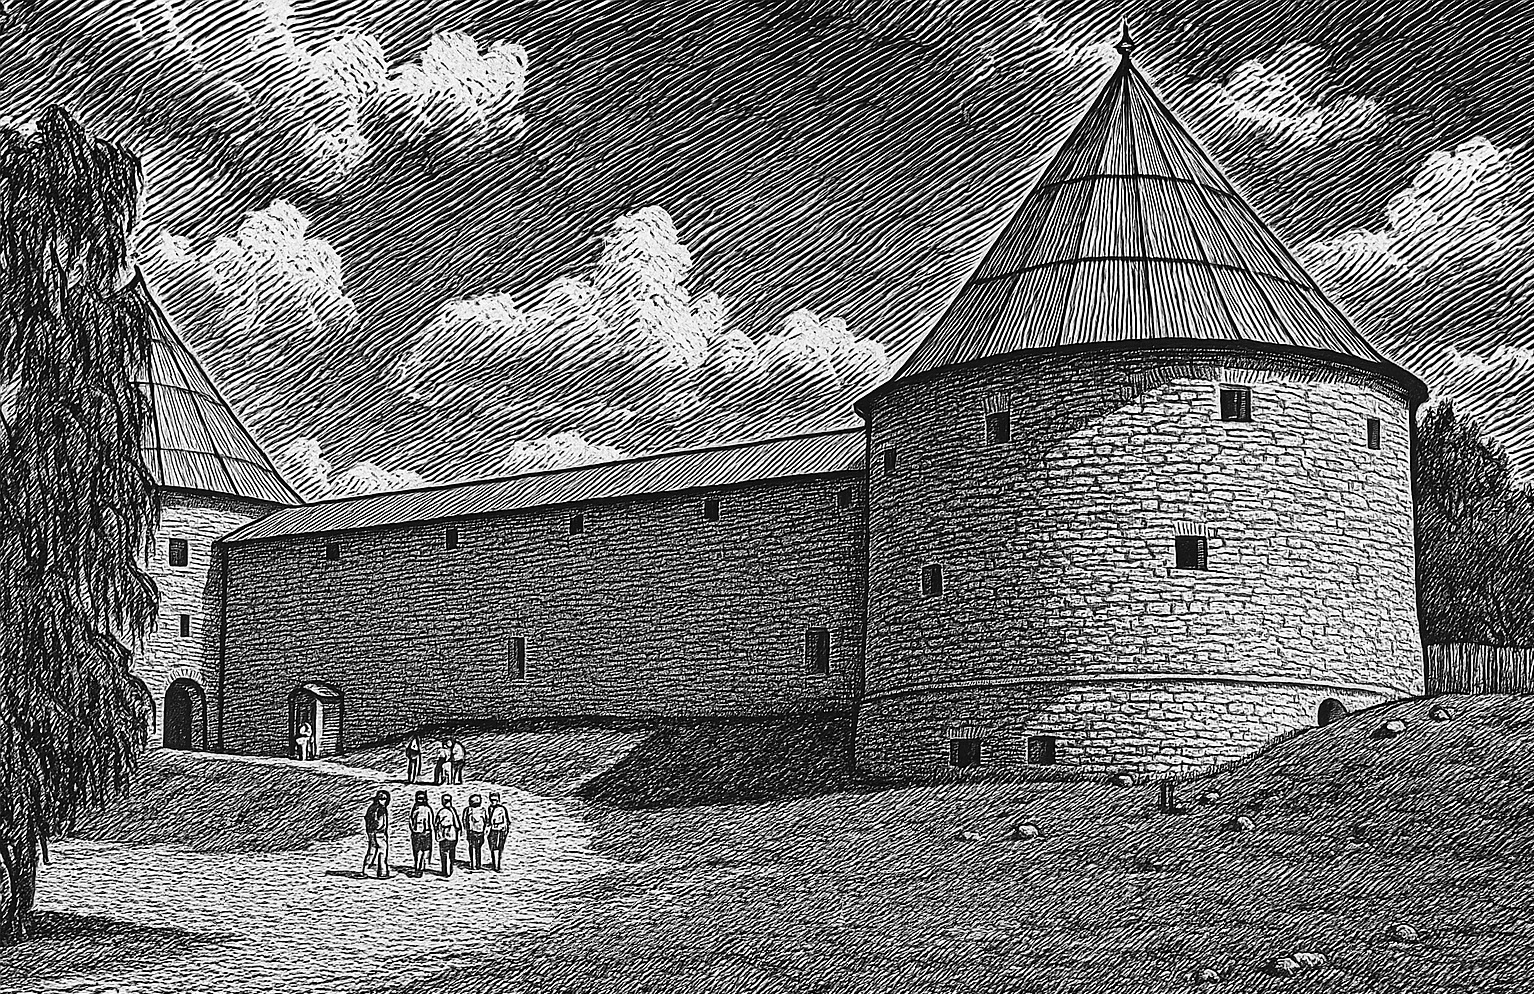
\includegraphics[width=1.0\textwidth]{07_ladoga}
	\caption{\small\textit{...нет, не скифы, не азиаты мы...}}
\end{figure}

%----------------------------------------------------------------
\newpage

text text

\noindent
\begin{minipage}{0.45\textwidth}
	\setlength{\parindent}{1.0cm}  % Восстановление отступа абзаца
	
	\indent Смотровая площадка располагалась после 4-й ступени водопада, самой высокой, а~немного выше был виден предыдущий каскад с~двумя чуть меньшими водопадиками. Друзья забрались в~самый дальний край тропинки на~гору, где была установлена лавочка и~открывался чудесный вид вниз на~долину. Присели на лавочку передохнуть и~подождать Серёгу с~Русланом.
	
	\indent Кивач\mdash жемчужина Карелии. Заповедник был \makebox[\linewidth][s]{\noindent создан в~30\sdash ые годы XX\hspace{0.25em}в.}
\end{minipage}\hfill
\begin{minipage}{0.5\textwidth}
	\centering
	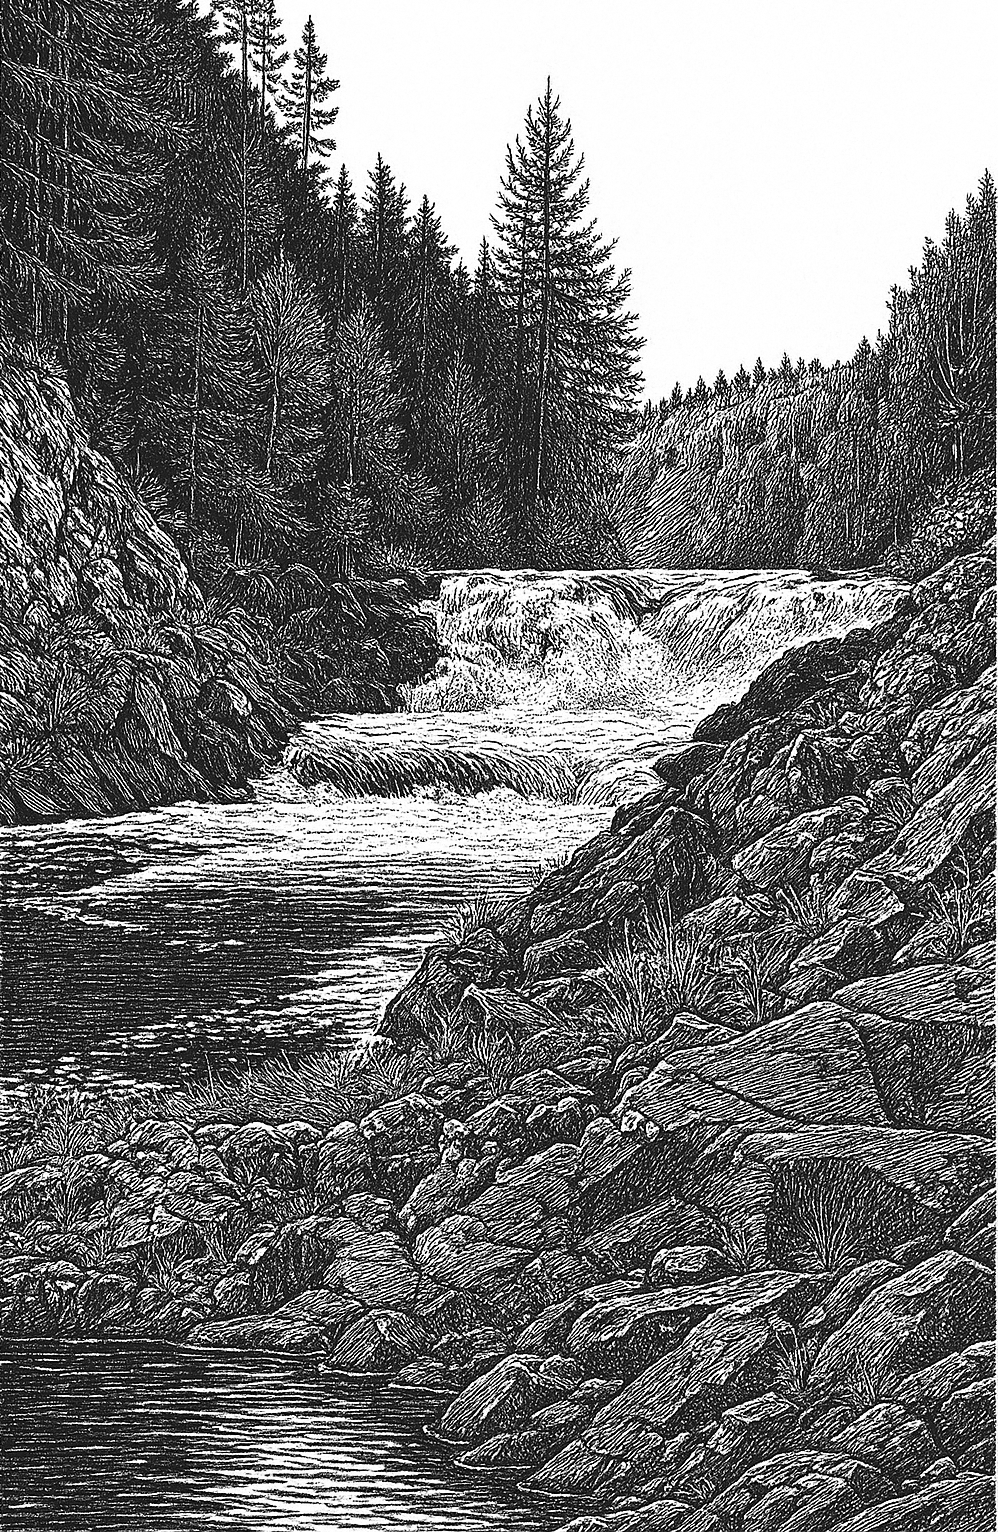
\includegraphics[width=\linewidth]{08_kivach}
	
	{\small\textit{...жемчужина Карелии...}}
\end{minipage}

%----------------------------------------------------------------
\newpage

\begin{figure}[h]
	\centering
	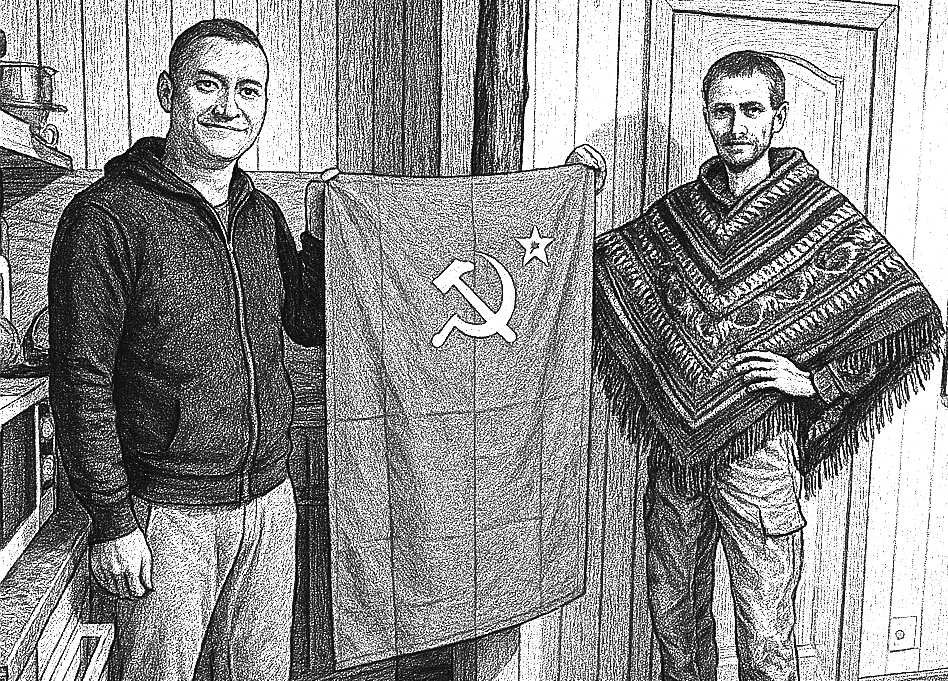
\includegraphics[width=1.0\textwidth]{09_2_ussr}
	\caption{\small\textit{...молоткасто-серпастое...}}
\end{figure}

%----------------------------------------------------------------
% 6 ГЛАВА
%----------------------------------------------------------------
\newpage

\begin{figure}[h]
	\centering
	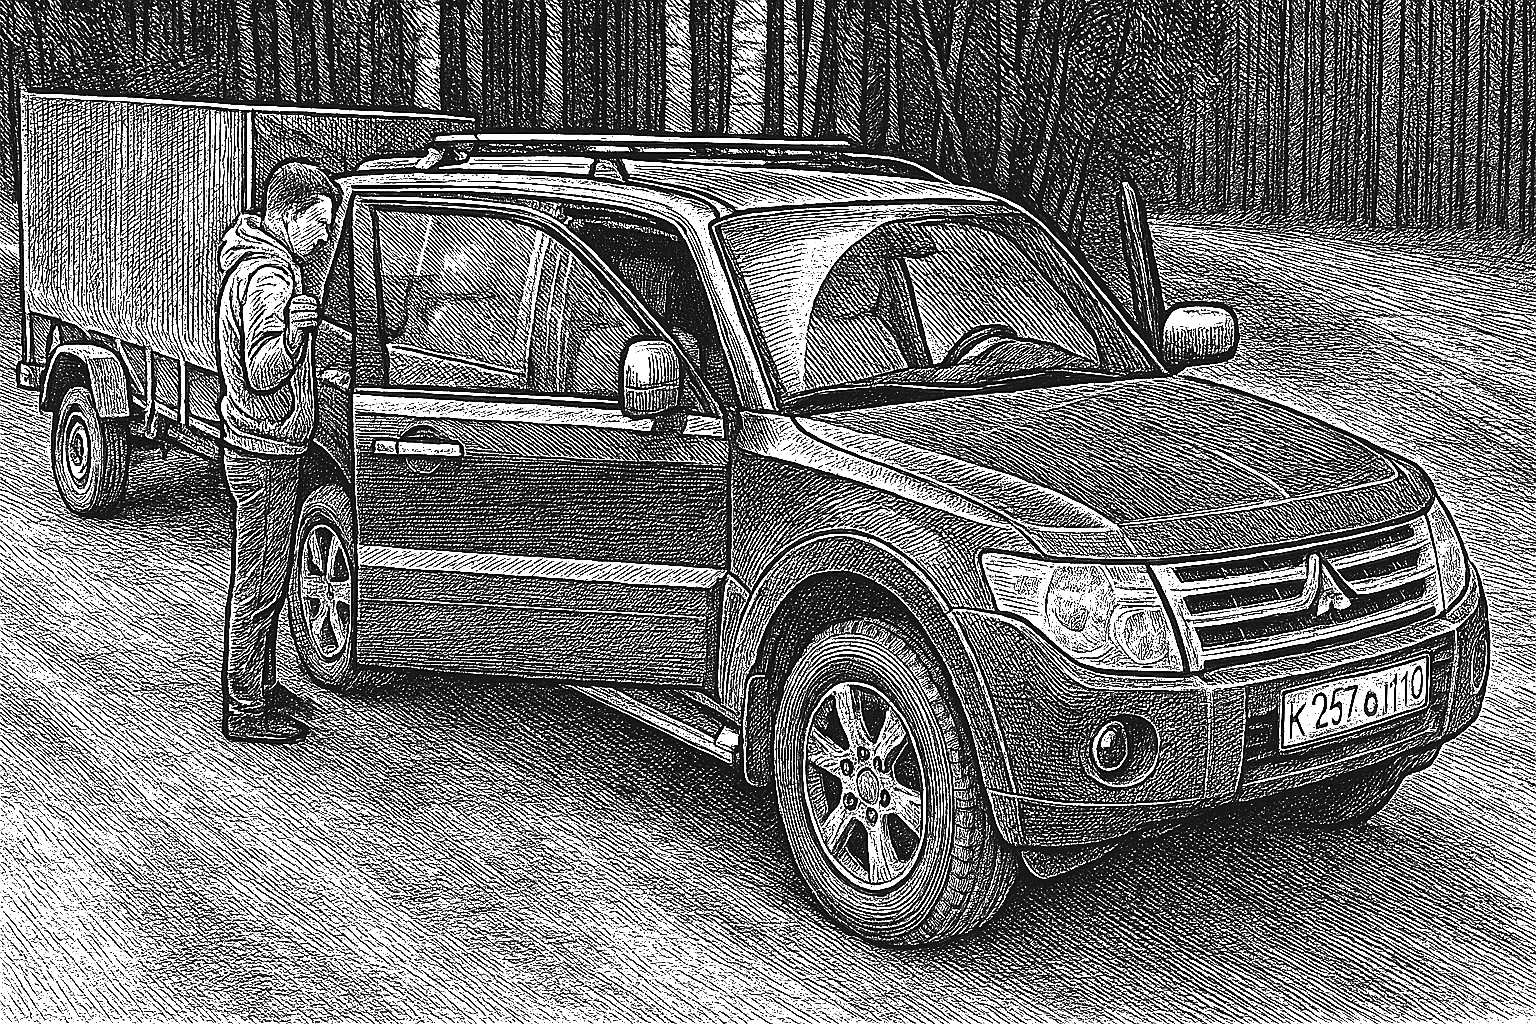
\includegraphics[width=1.0\textwidth]{10_1_jeep}
	\caption{\small\textit{...свернули направо на Нёлгомозеро...}}
\end{figure}

abcd

\begin{figure}[h]
	\centering
	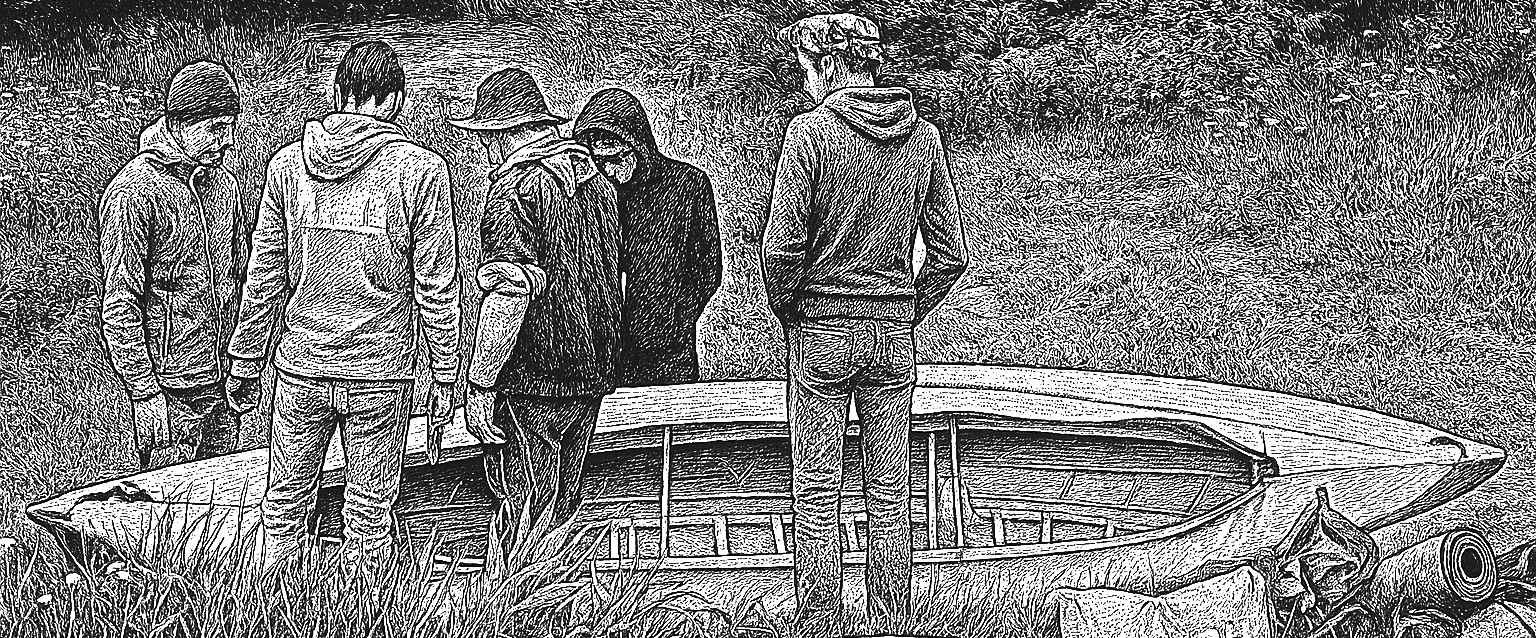
\includegraphics[width=1.0\textwidth]{11_1_keelson}
	\caption{\small\textit{...фальшборт не лезет...}}
\end{figure}

%----------------------------------------------------------------
\newpage

\begin{figure}[h]
	\centering
	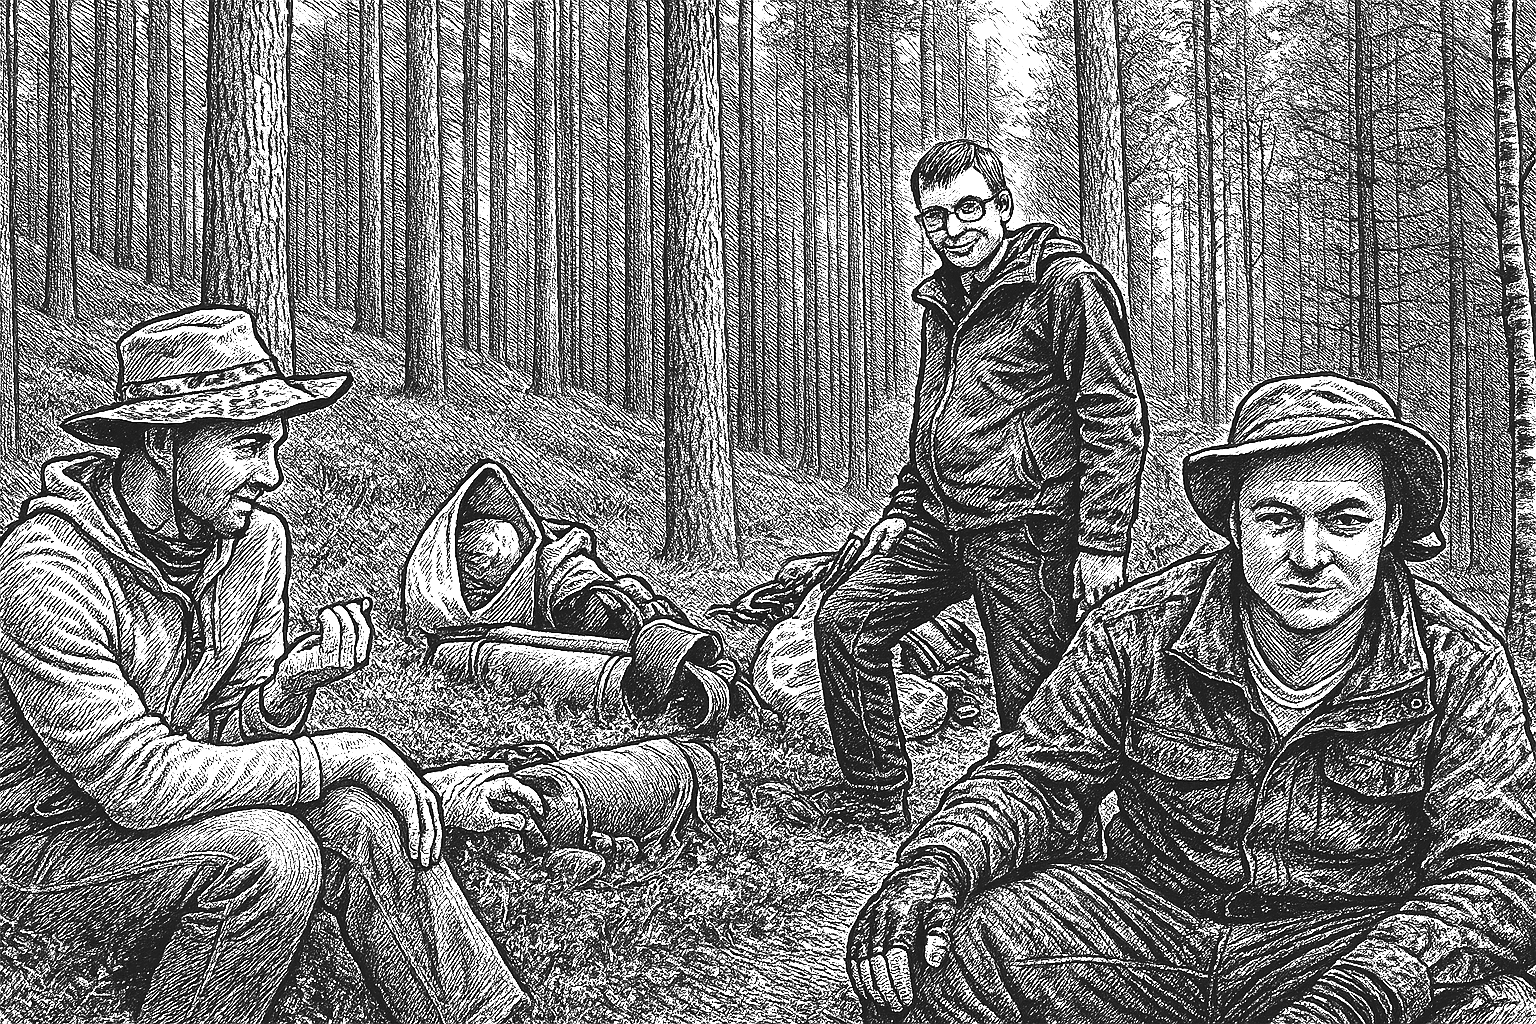
\includegraphics[width=1.0\textwidth]{12_1_maybe}
	\caption{\small\textit{...А чё, давайте может?...}}
\end{figure}

abcd

\newpage

\begin{wrapfigure}[10]{l}{0.52\textwidth}
	\setlength{\belowcaptionskip}{-10pt}
	%	\begin{figure}[h]
		\centering
		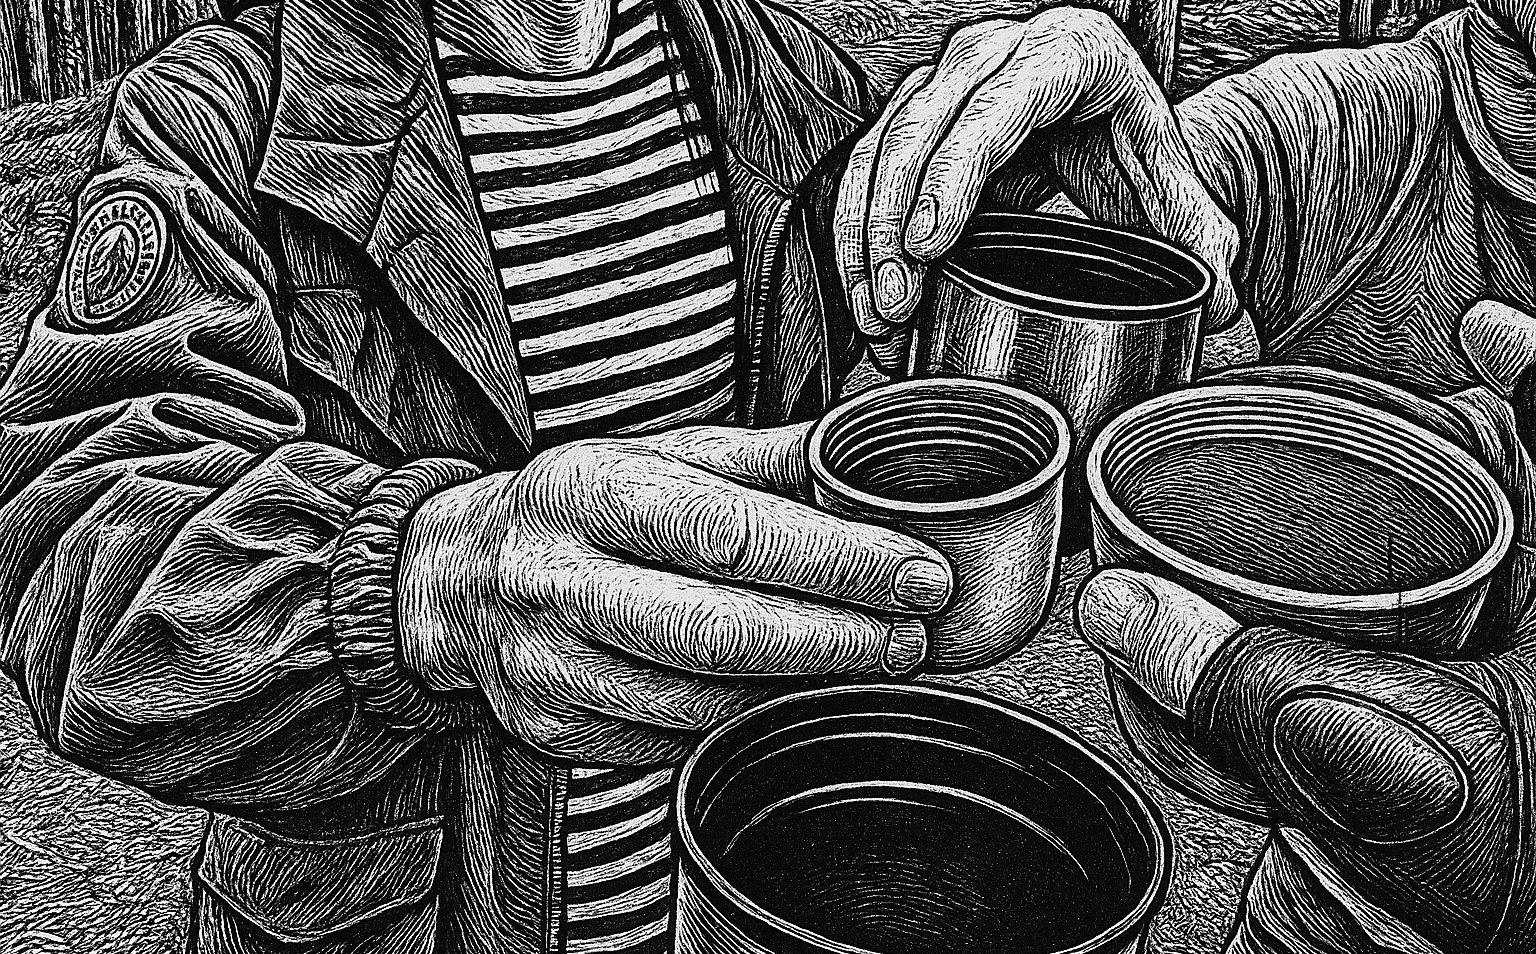
\includegraphics[width=0.52\textwidth]{13_skol}
		\caption{\small\textit{...два отрывистых...}}
		%	\end{figure}
\end{wrapfigure}

\noindent И сегодня нас ждут каналы между озёрами ещё, кстати. Итак, то, к~чему мы стремились\mdash свершается! Мы выбрались в наш первый совместный сплав по Карелии и, надеюсь, это приключение запомнится нам надолго! Ну,~мужики, будем!\mdash лес рук с кружками поднялся и замер, ожидая команды.\mdash Тащ~Замполит, два отрывистых и одно раскатистое!!!

%----------------------------------------------------------------
% 7 ГЛАВА
%----------------------------------------------------------------
\newpage

\begin{figure}[h]
	\centering
	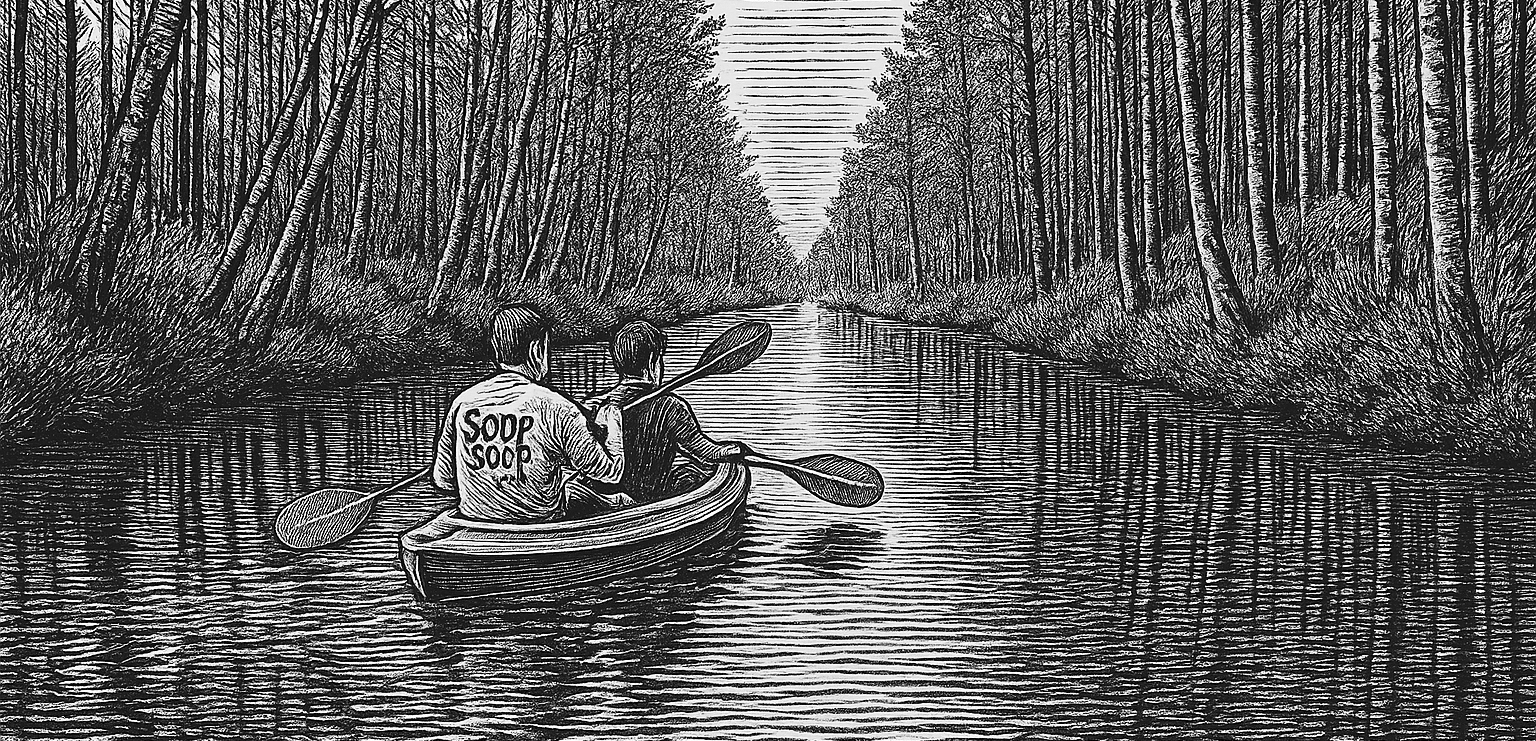
\includegraphics[width=1.0\textwidth]{14_channel}
	\caption{\small\textit{...Канал был шириной примерно метров 8...}}
\end{figure}

%----------------------------------------------------------------
\newpage

\begin{figure}[h]
	\centering
	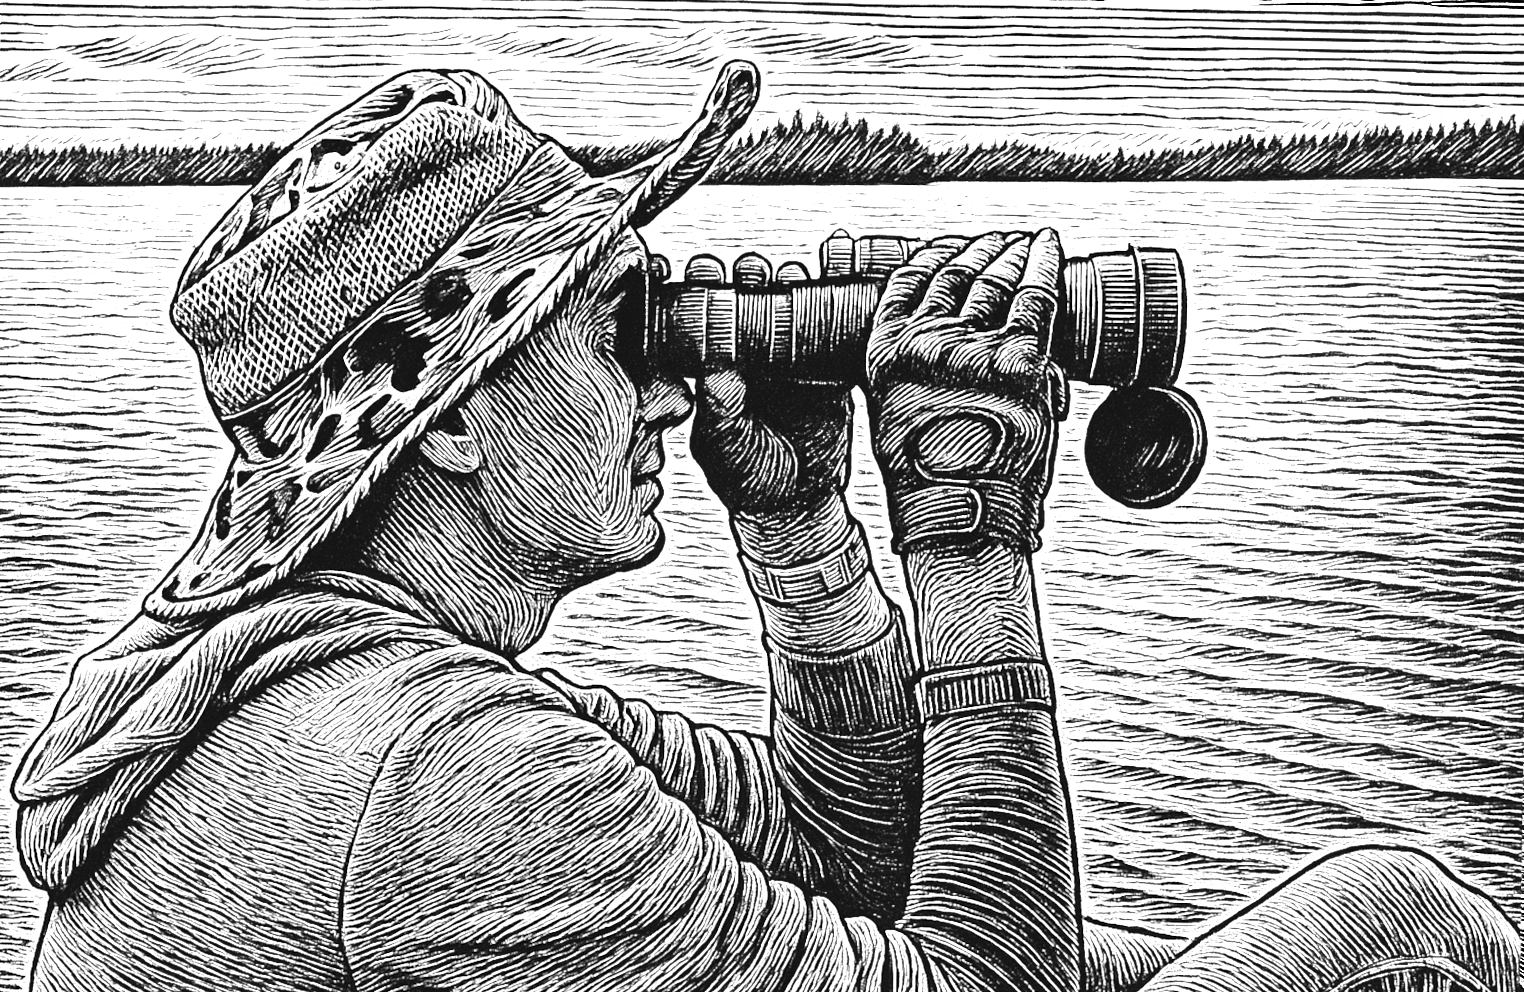
\includegraphics[width=1.0\textwidth]{15_1_okular}
	\caption{\small\textit{...ты говорил, что у тебя подзорная труба есть?...}}
\end{figure}

%----------------------------------------------------------------
% 8 ГЛАВА
%----------------------------------------------------------------
\newpage

\noindent
\begin{minipage}{0.38\textwidth}
	\setlength{\parindent}{1.0cm}  % Включаем красную строку
	\setlength{\parskip}{0.25cm}     % Межабзацный отступ, как в основном тексте
	
	\vspace{-0.4cm}
	\diagdash И\sdash и\sdash иха! 
	
	\diagdash ПОТАЩИЛО!!! --- Адмирал в полном восторге перестал грести веслом по\sdash байдарочному и~взял его под мышку на манер руля.\mdash Погнали!!!
	
	Ветер дул, конечно, не~особо сильный, но этого было вполне достаточно, чтобы дать им ход в~парочку км/ч. Второй экипаж, тем временем, наконец\sdash то отчалил и~догнал их:
\end{minipage}\hfill
\begin{minipage}{0.57\textwidth}
	\centering
	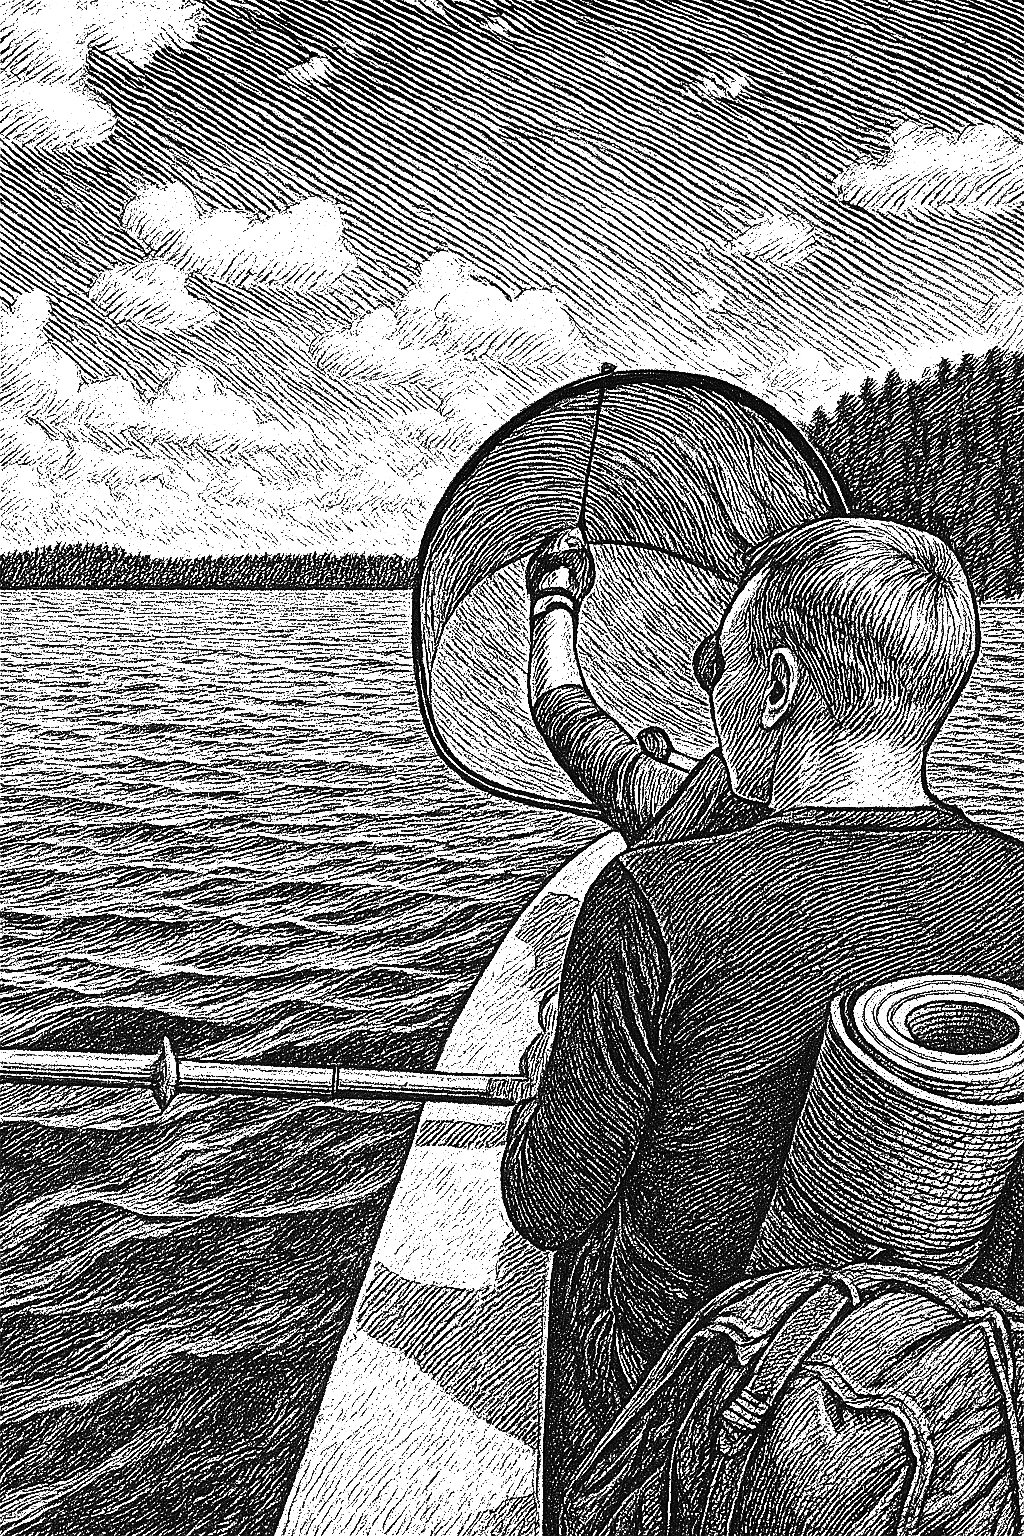
\includegraphics[width=0.95\linewidth]{16_1_parus}
	
	{\small\textit{...ветер стал усиливаться...}}
\end{minipage}

%----------------------------------------------------------------
\newpage

\begin{wrapfigure}[20]{r}{0.55\textwidth}
	%\begin{figure}[h]
	\centering
	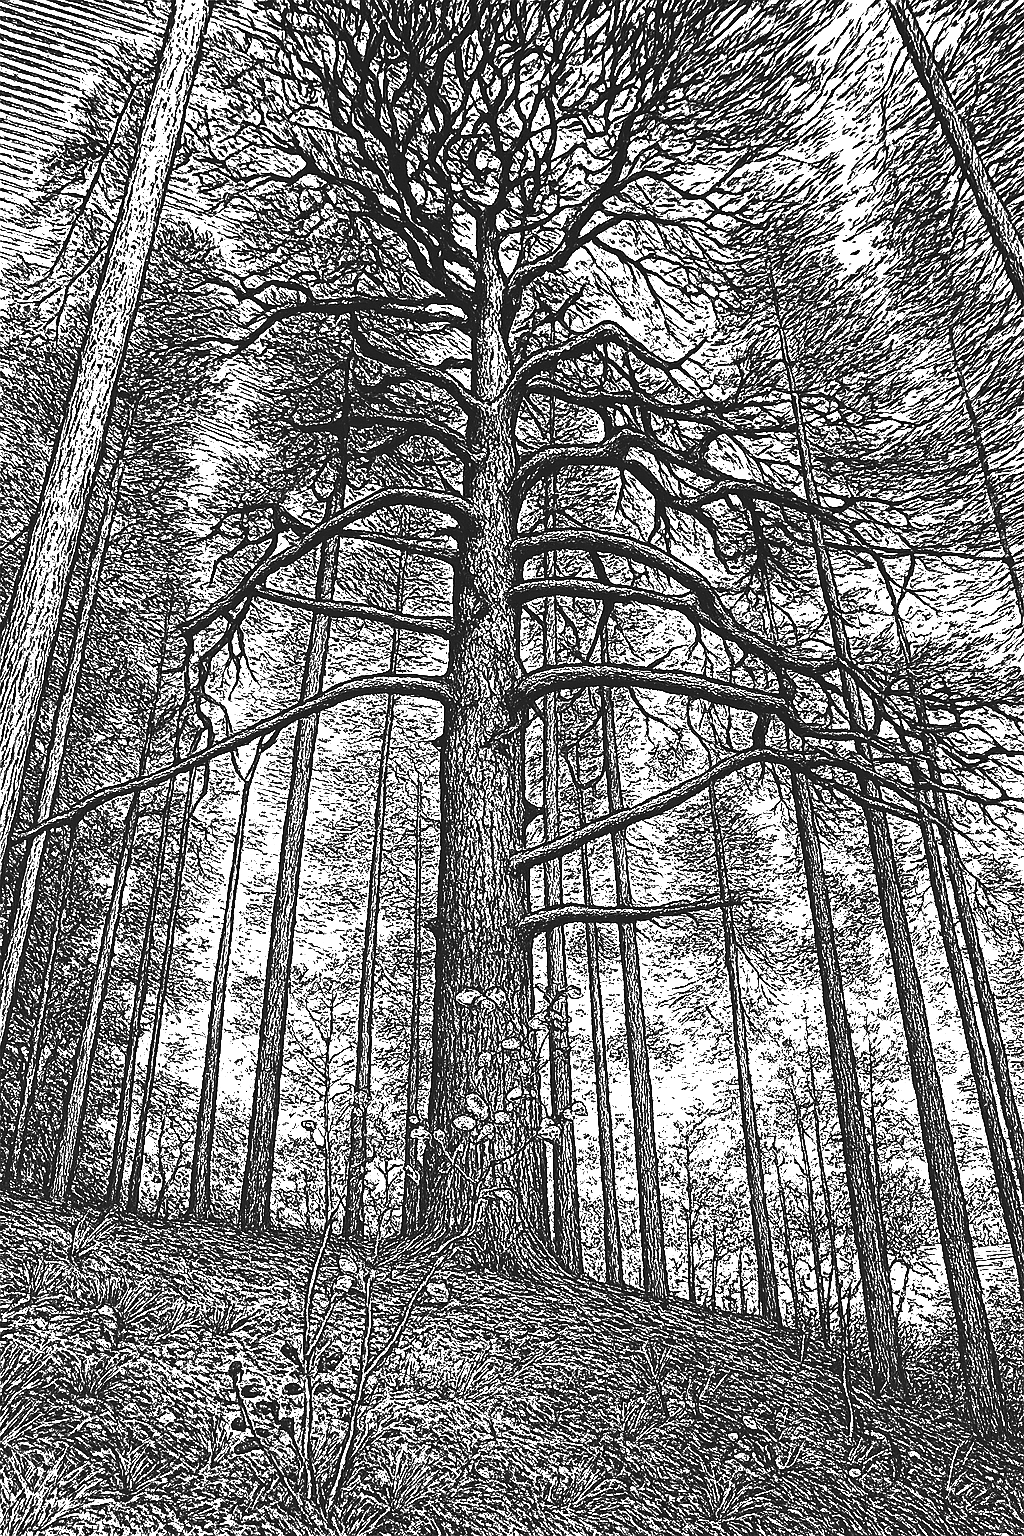
\includegraphics[width=0.55\textwidth]{17_2_tree}
	\caption{\small\textit{...Мы нашли Иггдрасиль!...}}
	%\end{figure}
\end{wrapfigure}
\diagdash Ваще похоже$\ldots$

\diagdash Шурик, там это, ясень был, у~скандинавов.\mdash сказал подошедший Киря.

\diagdash А у нас сосна будет! Она роднее как\sdash то. Мне всегда нравилась такая мифология\mdash древнегреческая и~древнеримская, потом древнескандинавская$\ldots$ Красиво они всё расписывали, черти!

\diagdash Да ты язычник?

\diagdash Это церковники христианские очернить чтобы придумали\mdash язычники, язычники, тьфу! У меня настольная книга была в школе\mdash <<Легенды и мифы Древней Греции и~Древнего Рима>>\cite{Кун}. Потом на~Скандинавию переключился$\ldots$ Красиво же!

%----------------------------------------------------------------
\newpage

\begin{figure}[h]
	\centering
	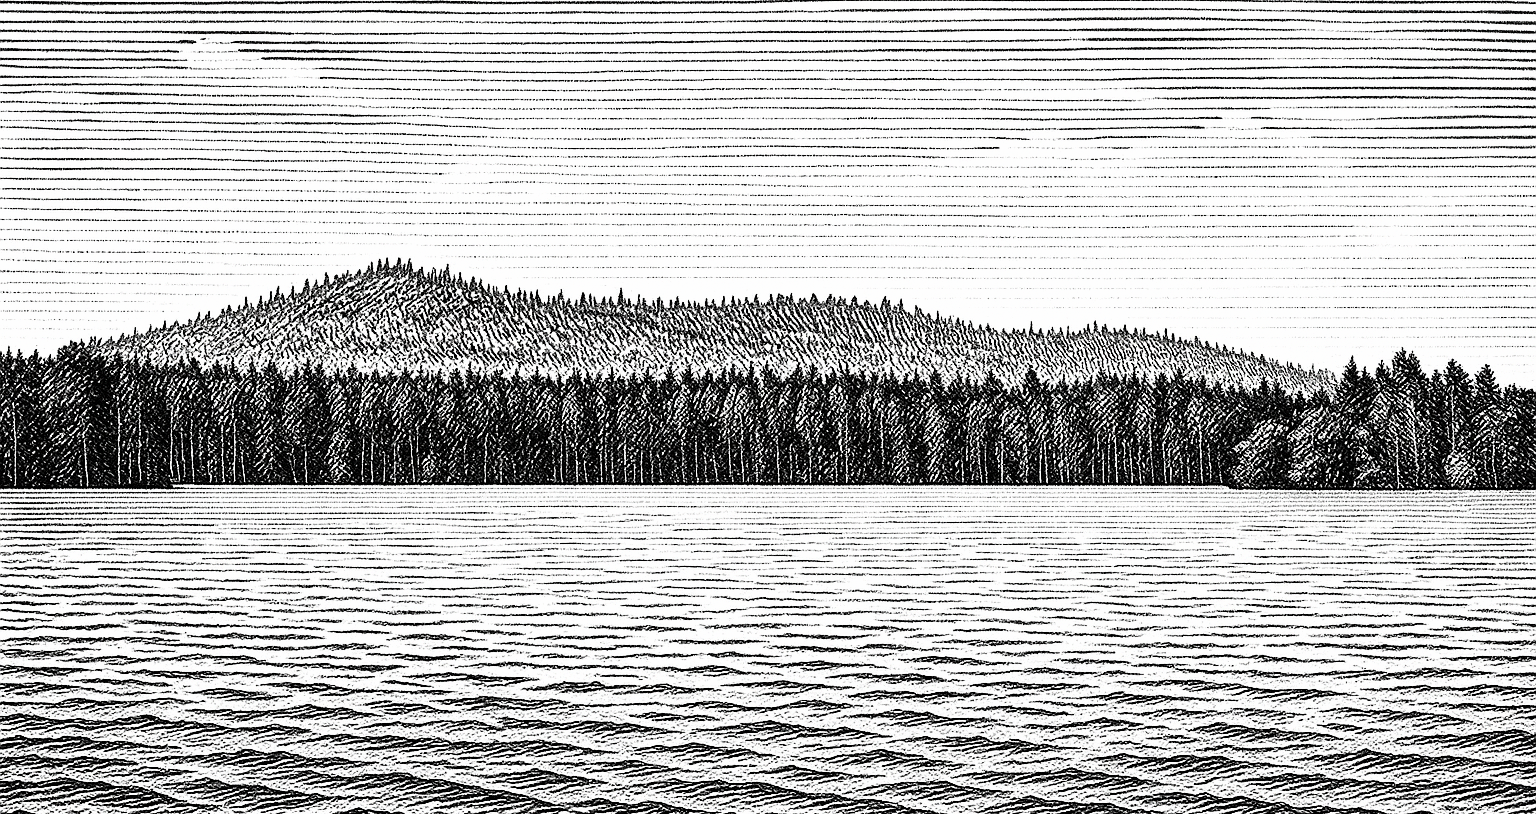
\includegraphics[width=1.0\textwidth]{18_mountain}
	\caption{\small\textit{...На~горизонте виднелась гора Ундойвара...}}
\end{figure}

\begin{wrapfigure}[11]{r}{0.45\textwidth}
	%\begin{figure}[h]
	\centering
	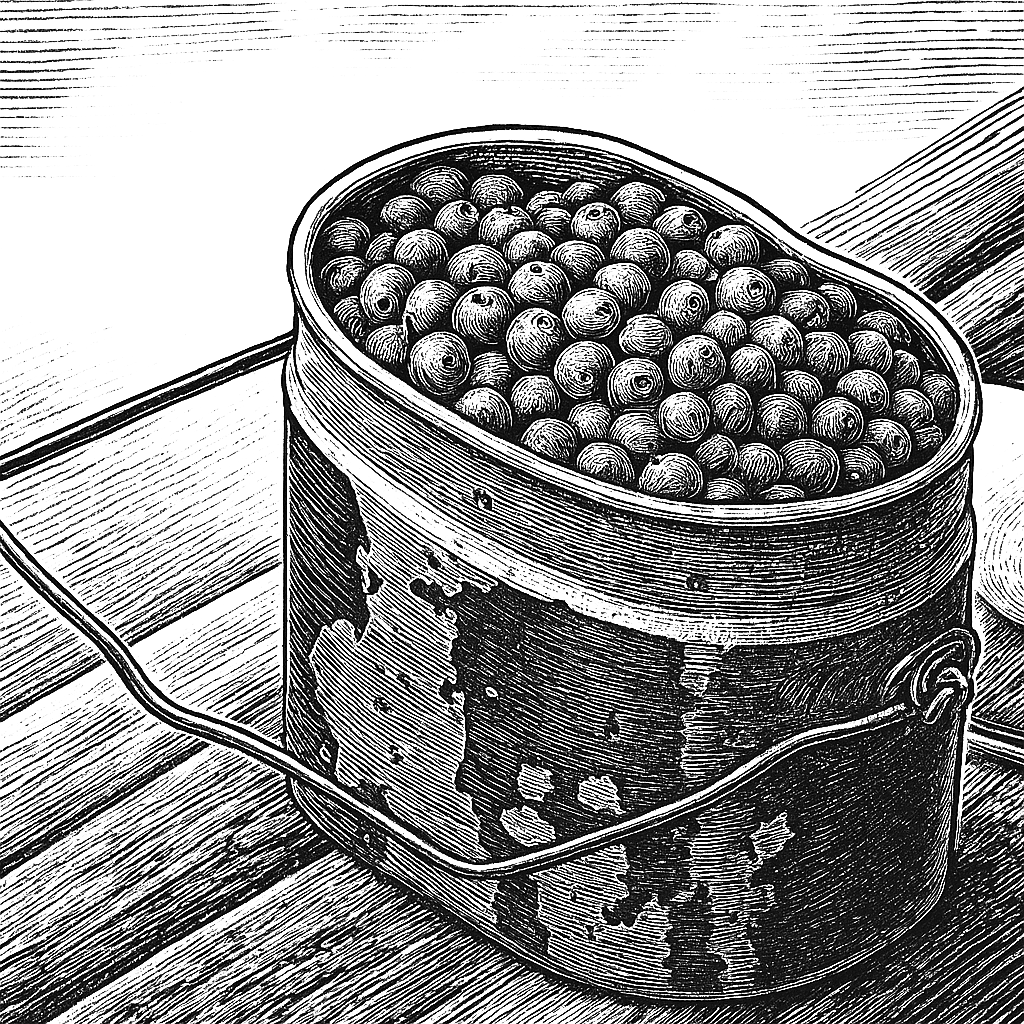
\includegraphics[width=0.45\textwidth]{19_1_blueberry}
	\caption{\small\textit{...Полный котелок черники...}}
	%\end{figure}
\end{wrapfigure}

%----------------------------------------------------------------
\newpage

\diagdash Не, парни, только троекратное <<УРА>> или <<SKÅL>>!\mdash Адмирал взял дольку апельсинчика.

%\diagdash Не, парни, только расово\sdash чистое троекратное <<УРА>> или <<SKÅL>>!\mdash Адмирал взял апельсинчик.

\diagdash Пофиг, будем!\mdash лес железных кубков поднялся.

\diagdash Кампай!

\diagdash SKÅL! Ну тебя с этим <<кампаем>>! Давай компотик варить!\mdash Адмирал попробовал спелую чернику.

%----------------------------------------------------------------
\newpage

\begin{figure}[h]
	\centering
	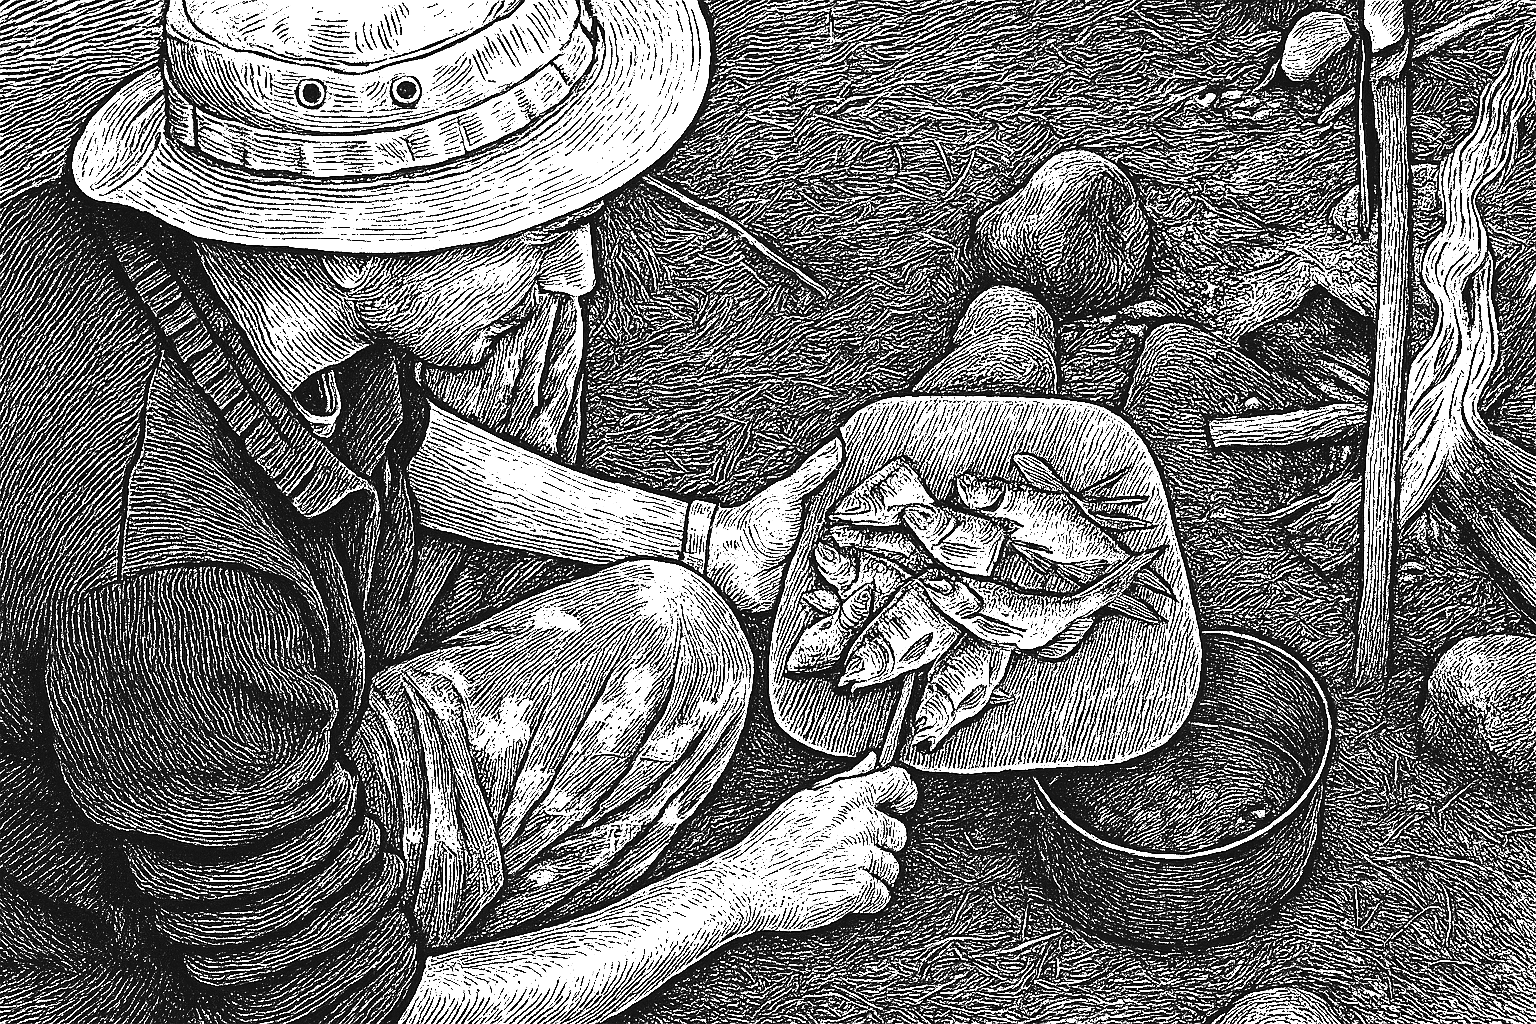
\includegraphics[width=1.0\textwidth]{20_1_fish}
	\caption{\small\textit{...А что там с супом?...}}
\end{figure}

%----------------------------------------------------------------
\newpage

\begin{figure}[h]
	\centering
	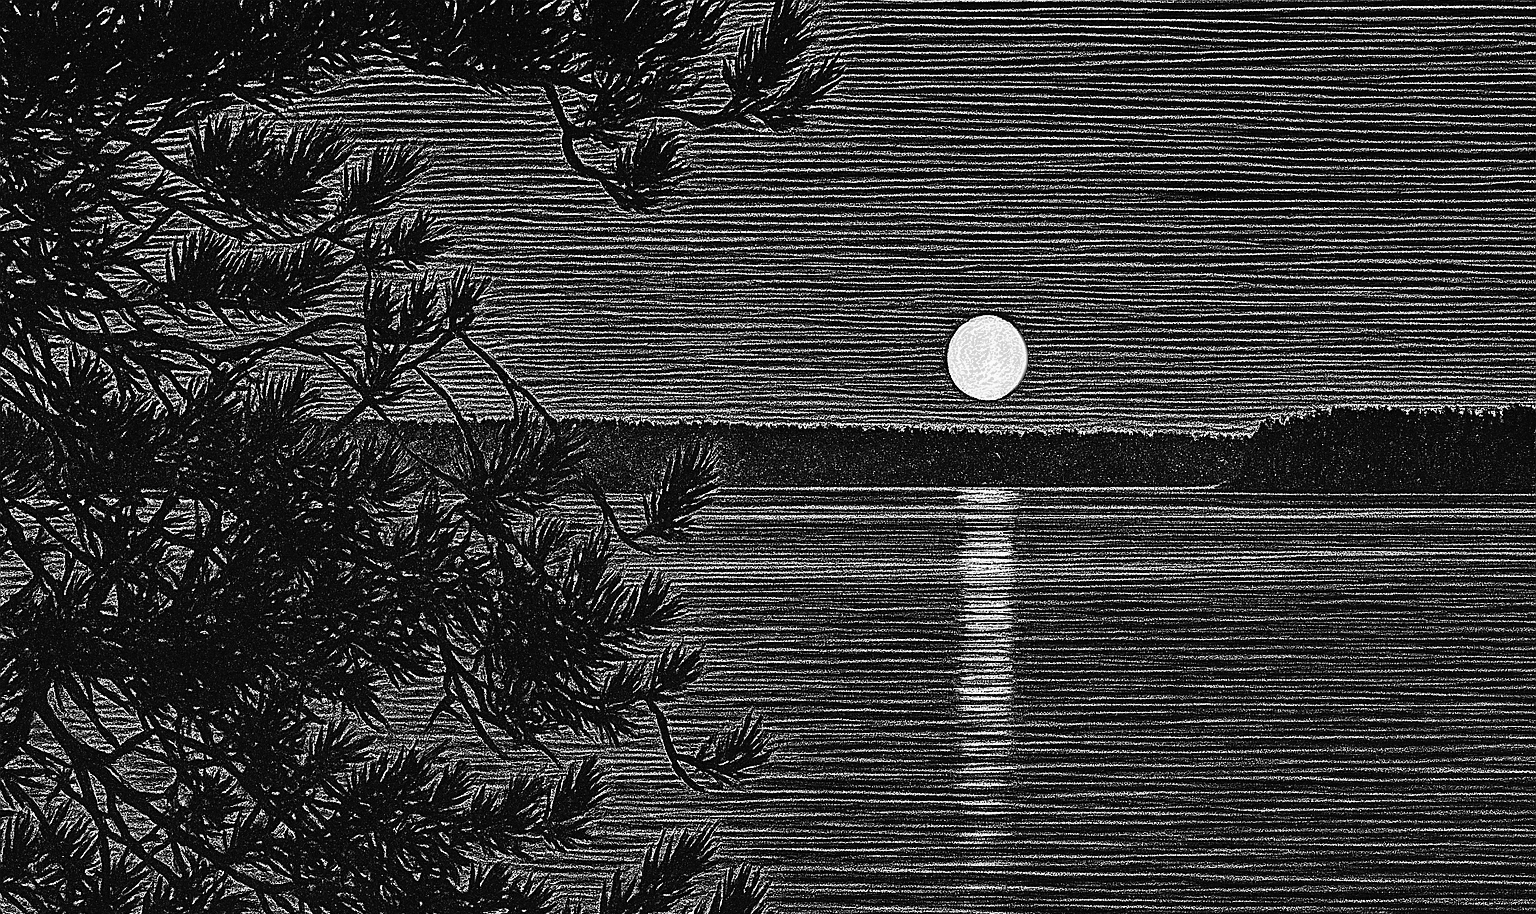
\includegraphics[width=1.0\textwidth]{21_moon.png}
	\caption{\small\textit{...Луна, взошедшая над лесом, отражалась в Мярандуксе...}}
\end{figure}

%----------------------------------------------------------------
% 9 ГЛАВА
%----------------------------------------------------------------
\newpage

\begin{figure}[h]
	\centering
	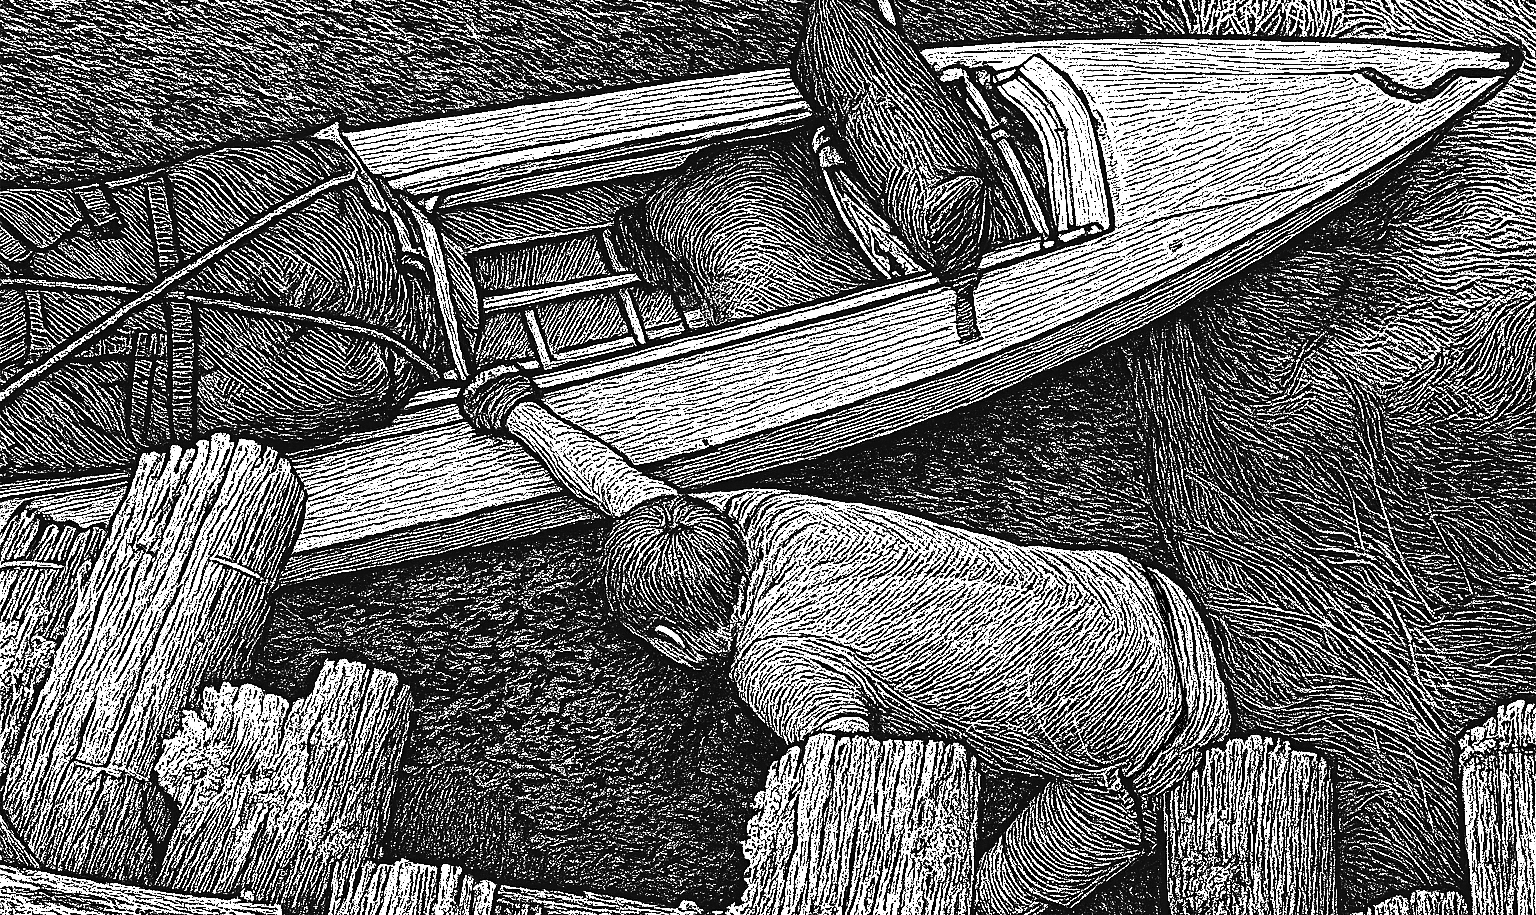
\includegraphics[width=1.0\textwidth]{22_1_serega}
	\caption{\small\textit{...Э-Э-Э!!!\mdash только и успел проорать Серёга...}}
\end{figure}

%----------------------------------------------------------------
\newpage

\begin{figure}[h]
	\centering
	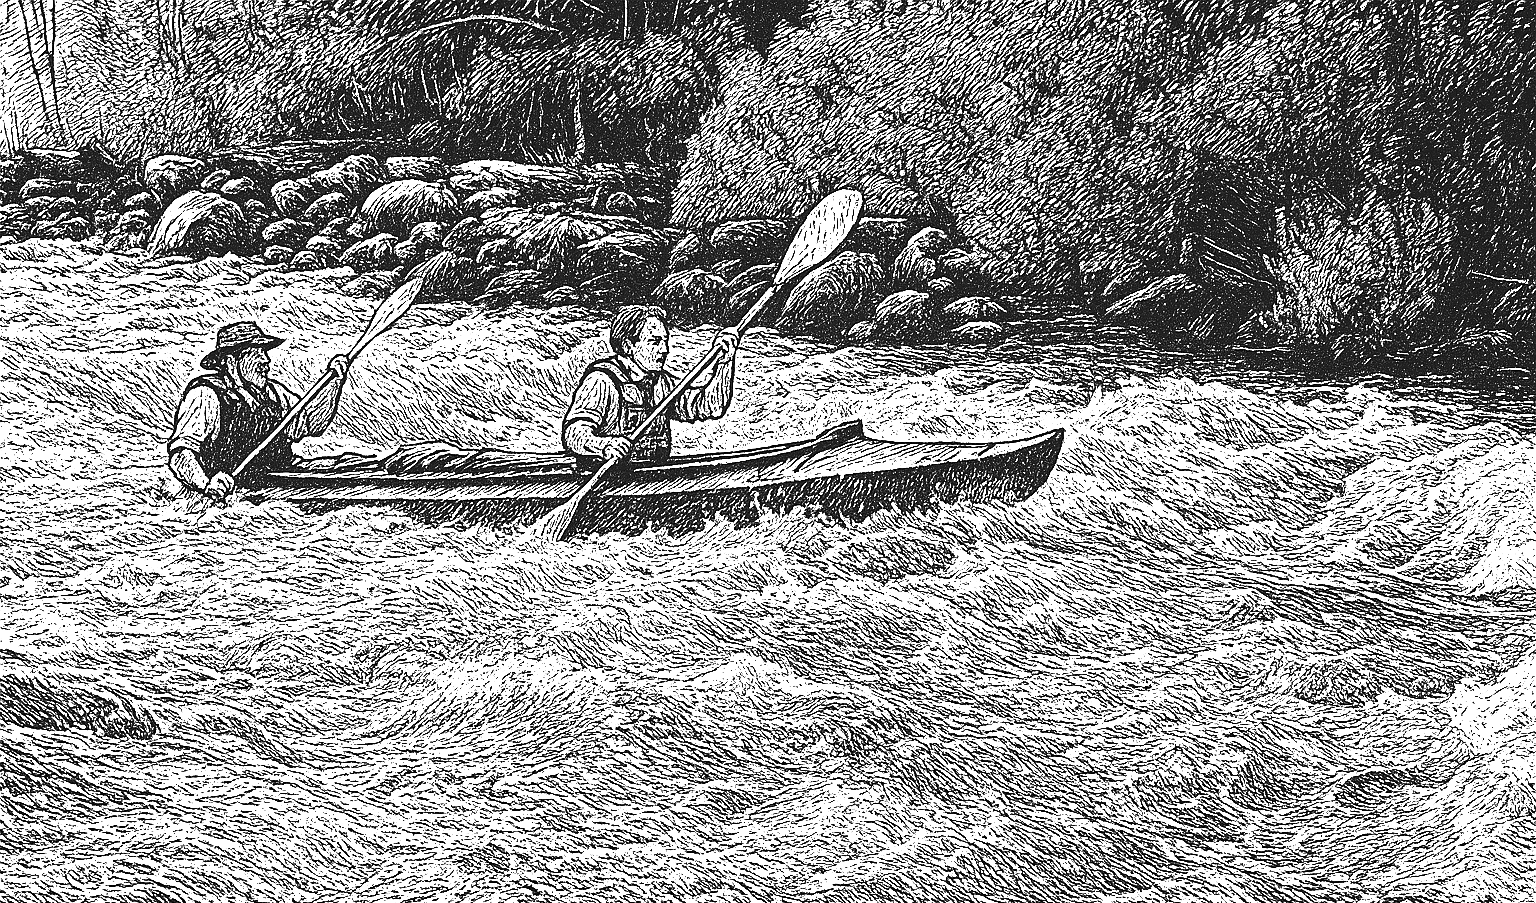
\includegraphics[width=1.0\textwidth]{23_1_fail}
	\caption{\small\textit{...Серёга!!! Левым!!!\mdash заорал Замполит...}}
\end{figure}

%----------------------------------------------------------------
\newpage

\begin{figure}[h]
	\centering
	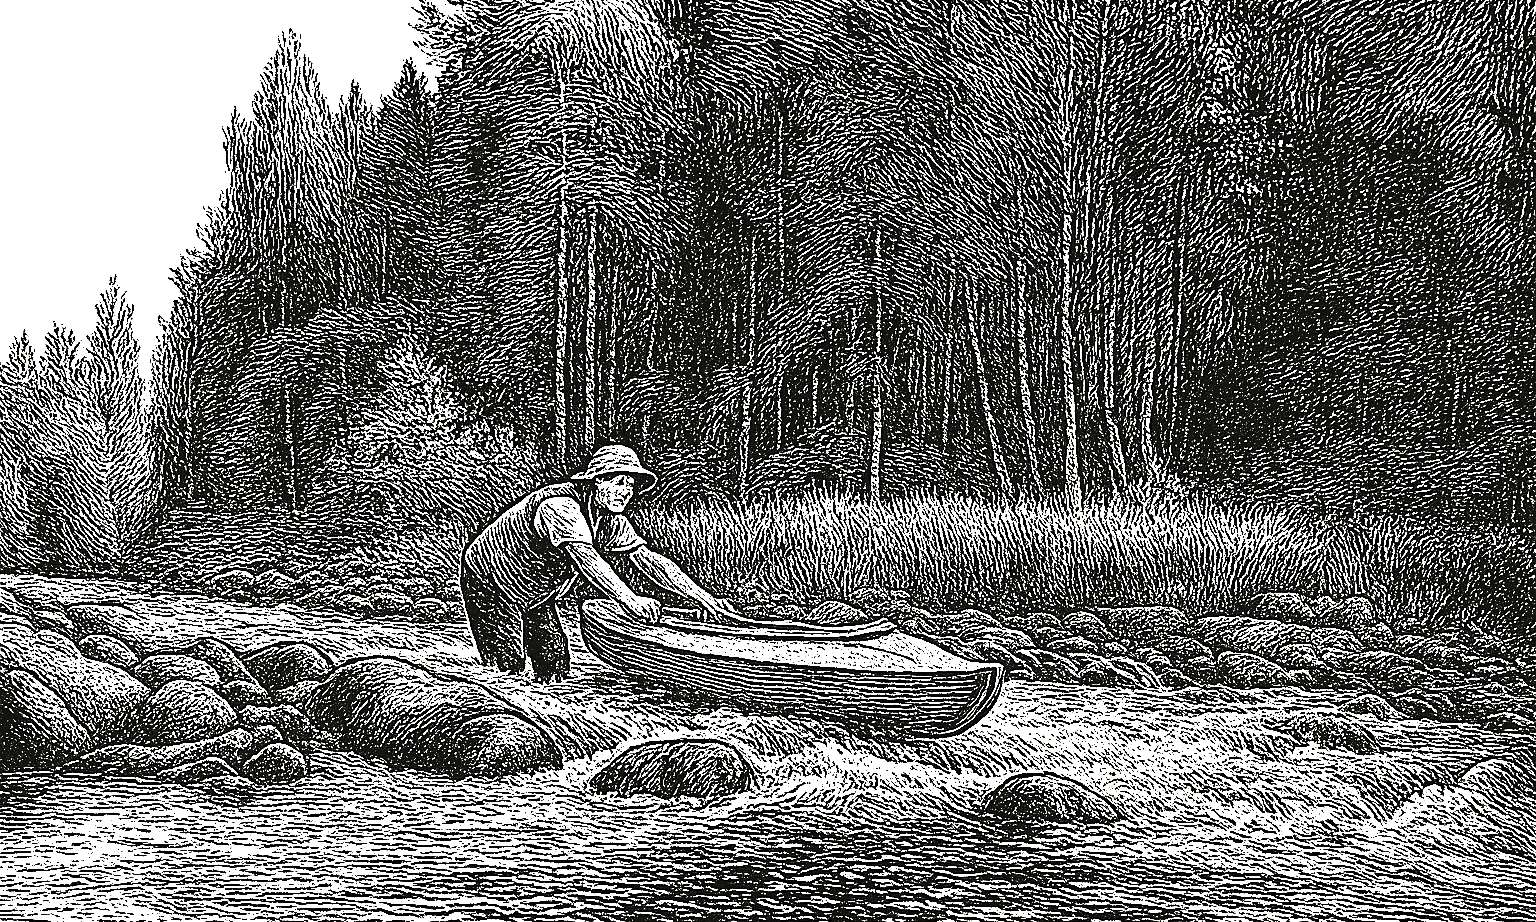
\includegraphics[width=1.0\textwidth]{24_1_nurmis}
	\caption{\small\textit{...пошли проводиться...}}
\end{figure}

%----------------------------------------------------------------
\newpage

\begin{figure}[h]
	\centering
	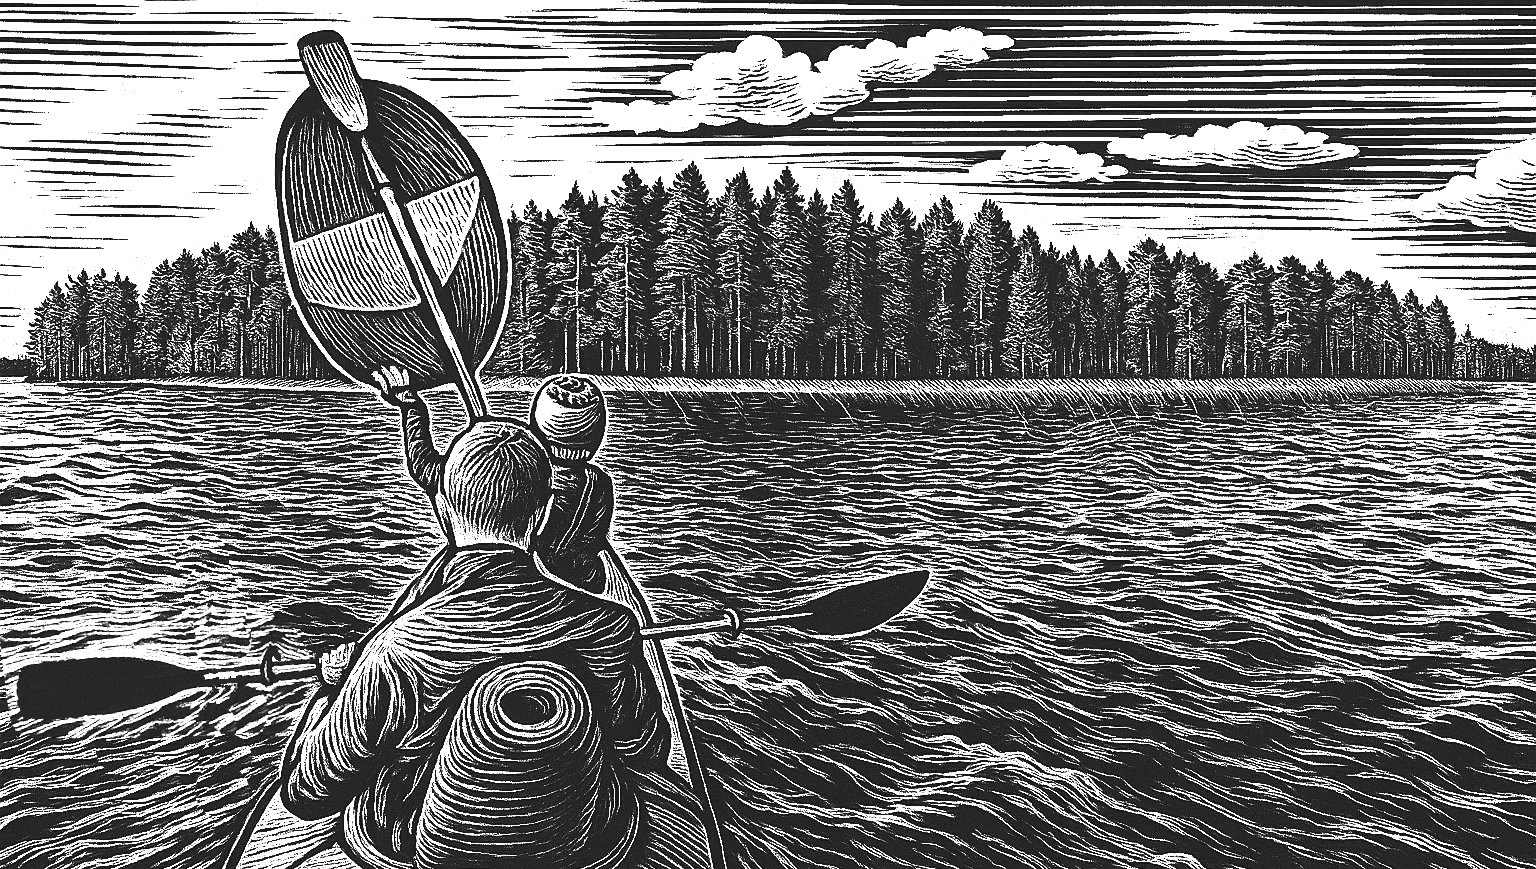
\includegraphics[width=1.0\textwidth]{25_1_island}
	\caption{\small\textit{...Ветер стремительно тащил их вперёд к острову...}}
\end{figure}

%----------------------------------------------------------------
\newpage

\begin{wrapfigure}[23]{l}{0.6\textwidth}
	%\begin{figure}[h]
	\centering
	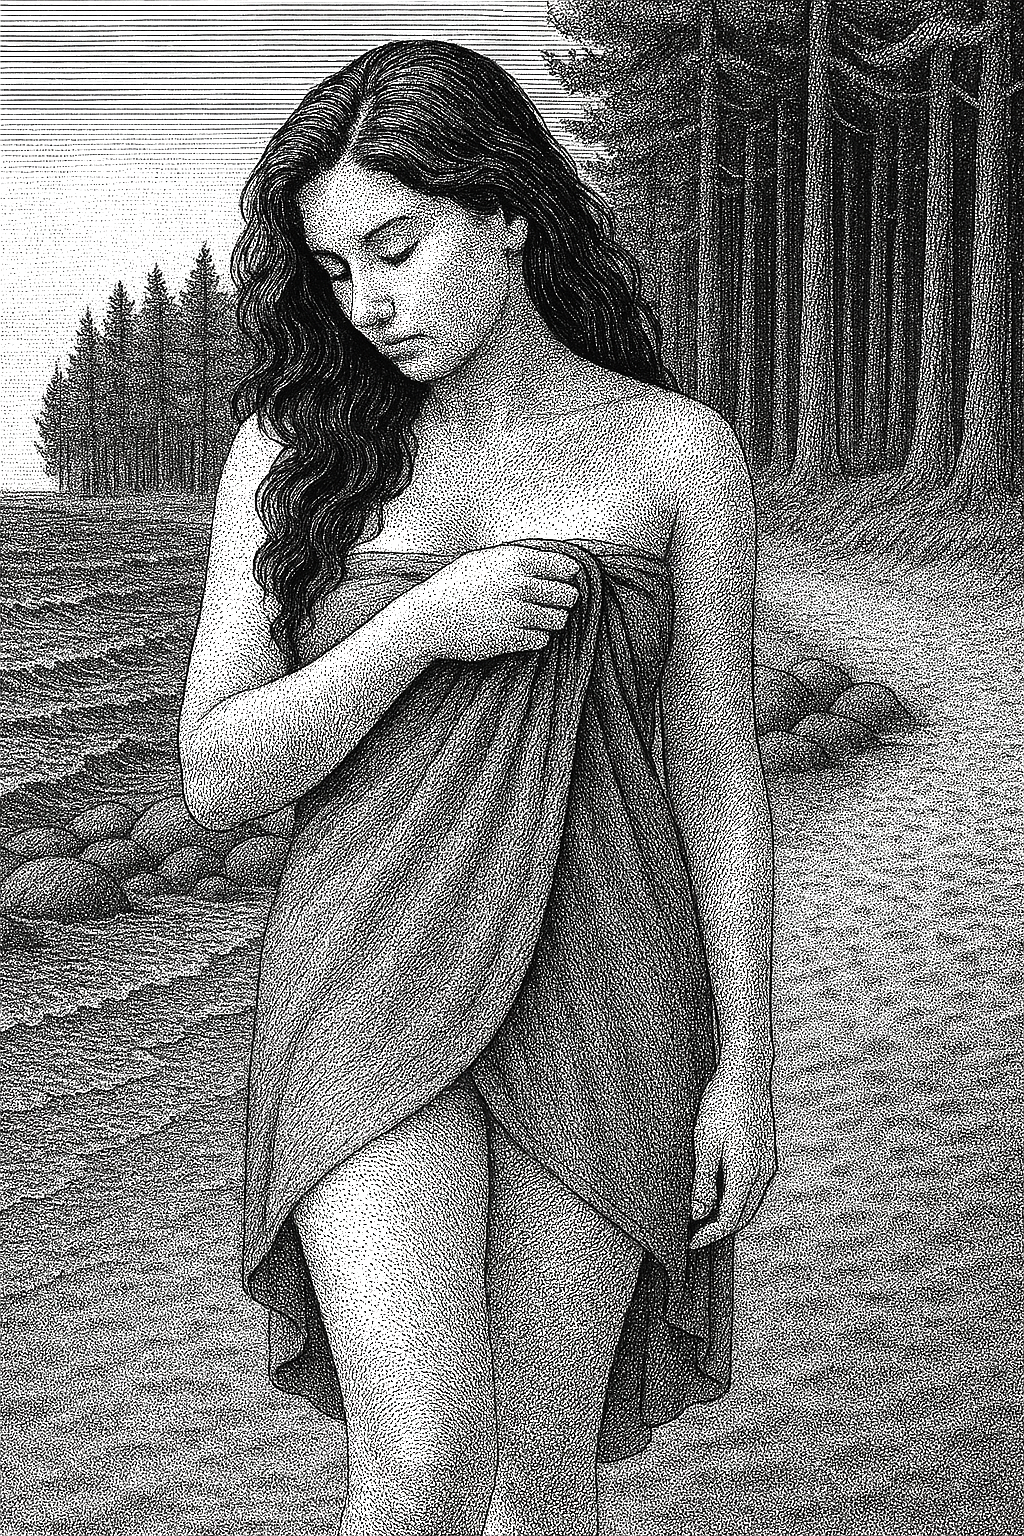
\includegraphics[width=0.6\textwidth]{26_4_valkyrie}
	\caption{\small\textit{...завернувшись в одно полотенце...}}
	%\end{figure}
\end{wrapfigure}

\diagdash Дьявол, да хар{\'о}ш уже!!!\mdash Адмирал начал грести по\sdash активнее, чтобы справиться с~нахлынувшим.

\diagdash Шурик, куда ты так гребёшь?%Дай насладиться\sdash то, ну?

\diagdash Стоянку на днёвку ищем, или мне это снится?\mdash огрызнулся Адмирал.

\diagdash Ишь ты!\mdash Киря подрезал его на повороте,\mdash Хопа!\mdash и вышел вперёд.

\diagdash В заливчике давайте поглядим!\mdash Адмирал жадно вглядывался в~берег, они обогнули южный мыс и~зашли в~небольшую бухту.

%----------------------------------------------------------------
\newpage

\begin{wrapfigure}[23]{l}{0.6\textwidth}
	%\begin{figure}[h]
	\centering
	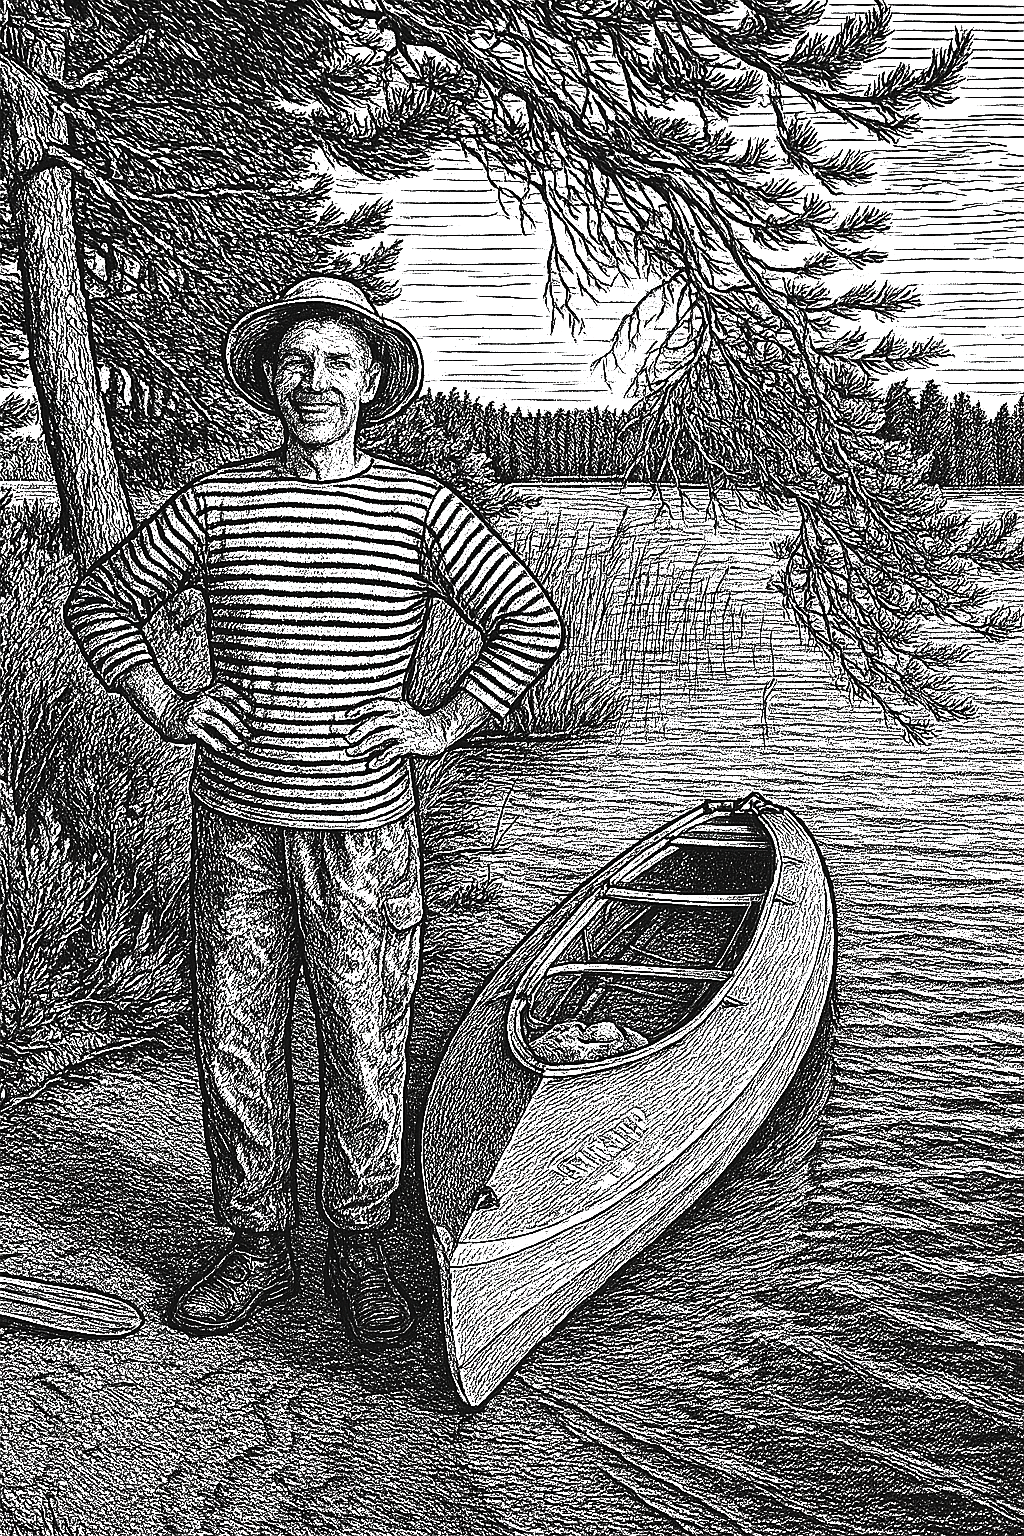
\includegraphics[width=0.6\textwidth]{27_1_shurik}
	\caption{\small\textit{...под сосной на берегу озера...}}
	%\end{figure}
\end{wrapfigure}

Вечер сгущался тёмный и~облачный. 
Над столом парни натянули тент, а к~соснам, росшим тут же, привалили гермы с продуктами и~вещмешки. 
%\begin{wrapfigure}[15]{l}{0.6\textwidth}
%\begin{figure}[h]
%	\centering
%	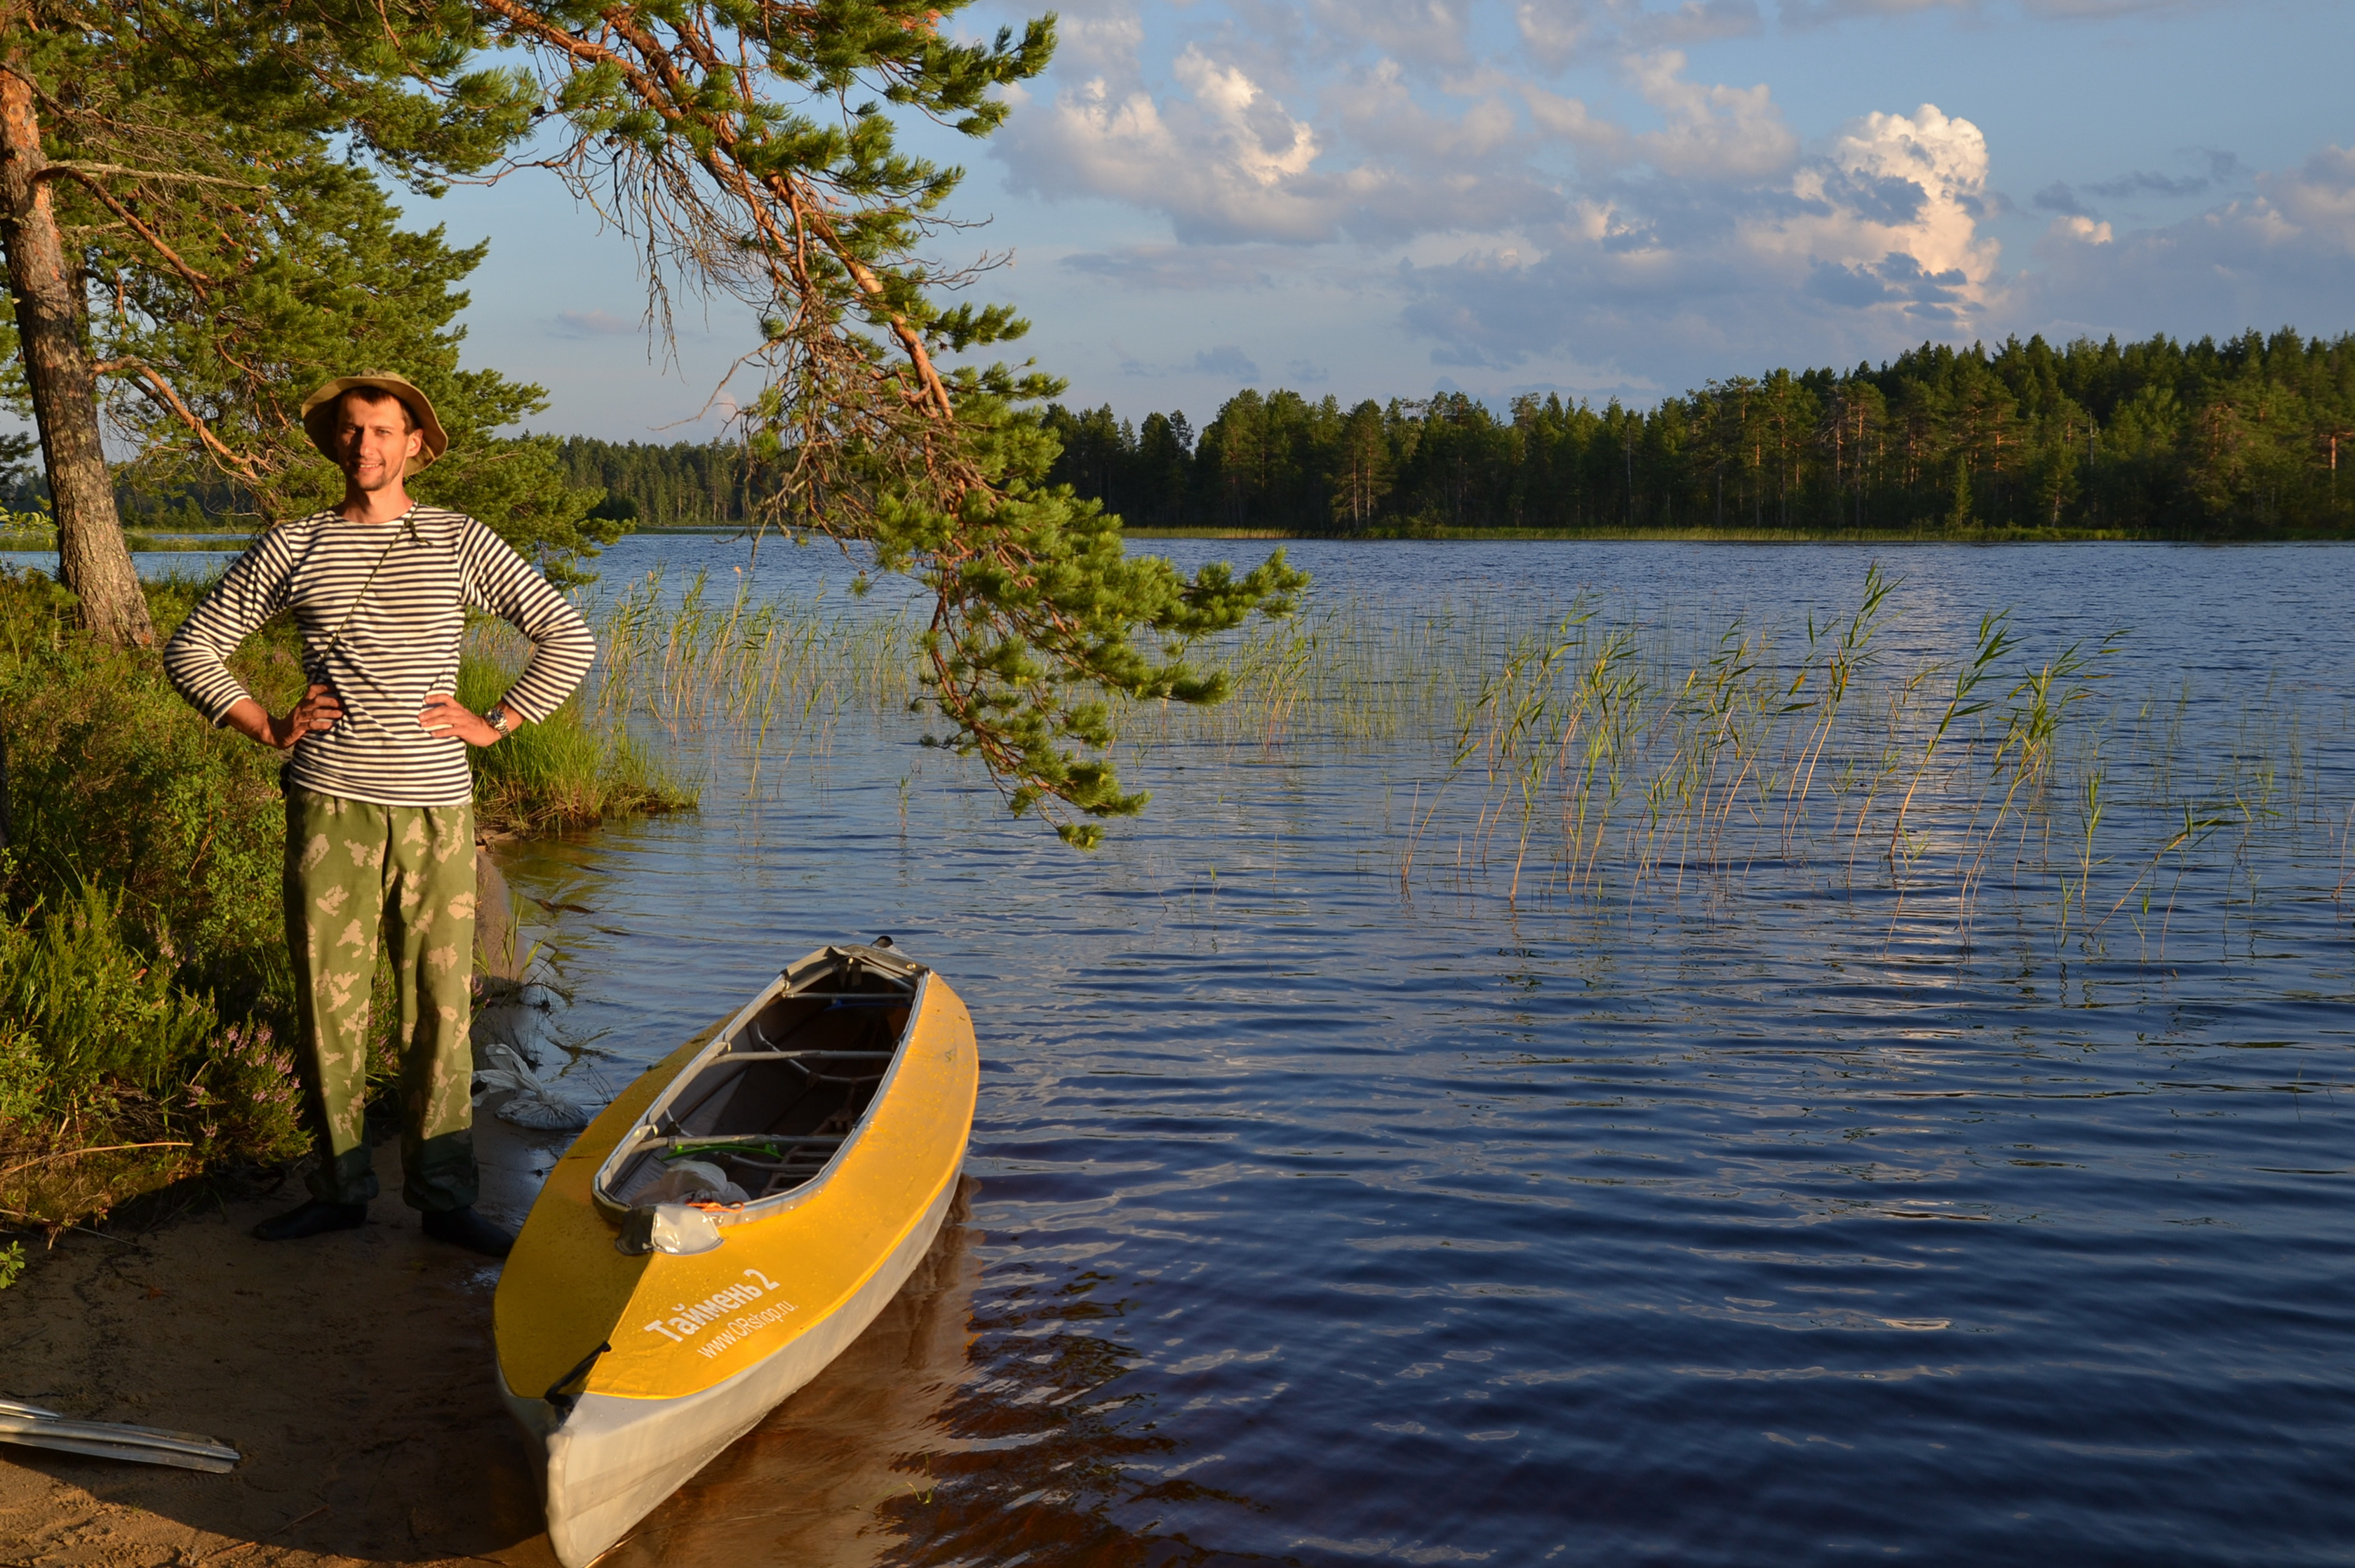
\includegraphics[width=1.0\textwidth]{9_4}
%	\caption{\small\textit{...пристали к берегу под сосной, росшей прям на берегу...}}
%\end{figure}
%\end{wrapfigure}
Костёр Адмирал мигом сообразил из имевшегося неподалёку валежника и отослал команду за нормальными дровами\mdash ему хотелось побыстрее сварить горячего.

Замполит~живо возглавил заготовку дров, дело спорилось\mdash у костра образовалась целая груда брёвен, что ребята притащили из леса. Котелки с водой уже пошумливали над костром, а Адмирал собрал свои походные кресла, уселся в~одно из них и распотрошил герму с~продуктами:

%----------------------------------------------------------------
% 10 ГЛАВА
%----------------------------------------------------------------
\newpage

\begin{figure}[h]
	\centering
	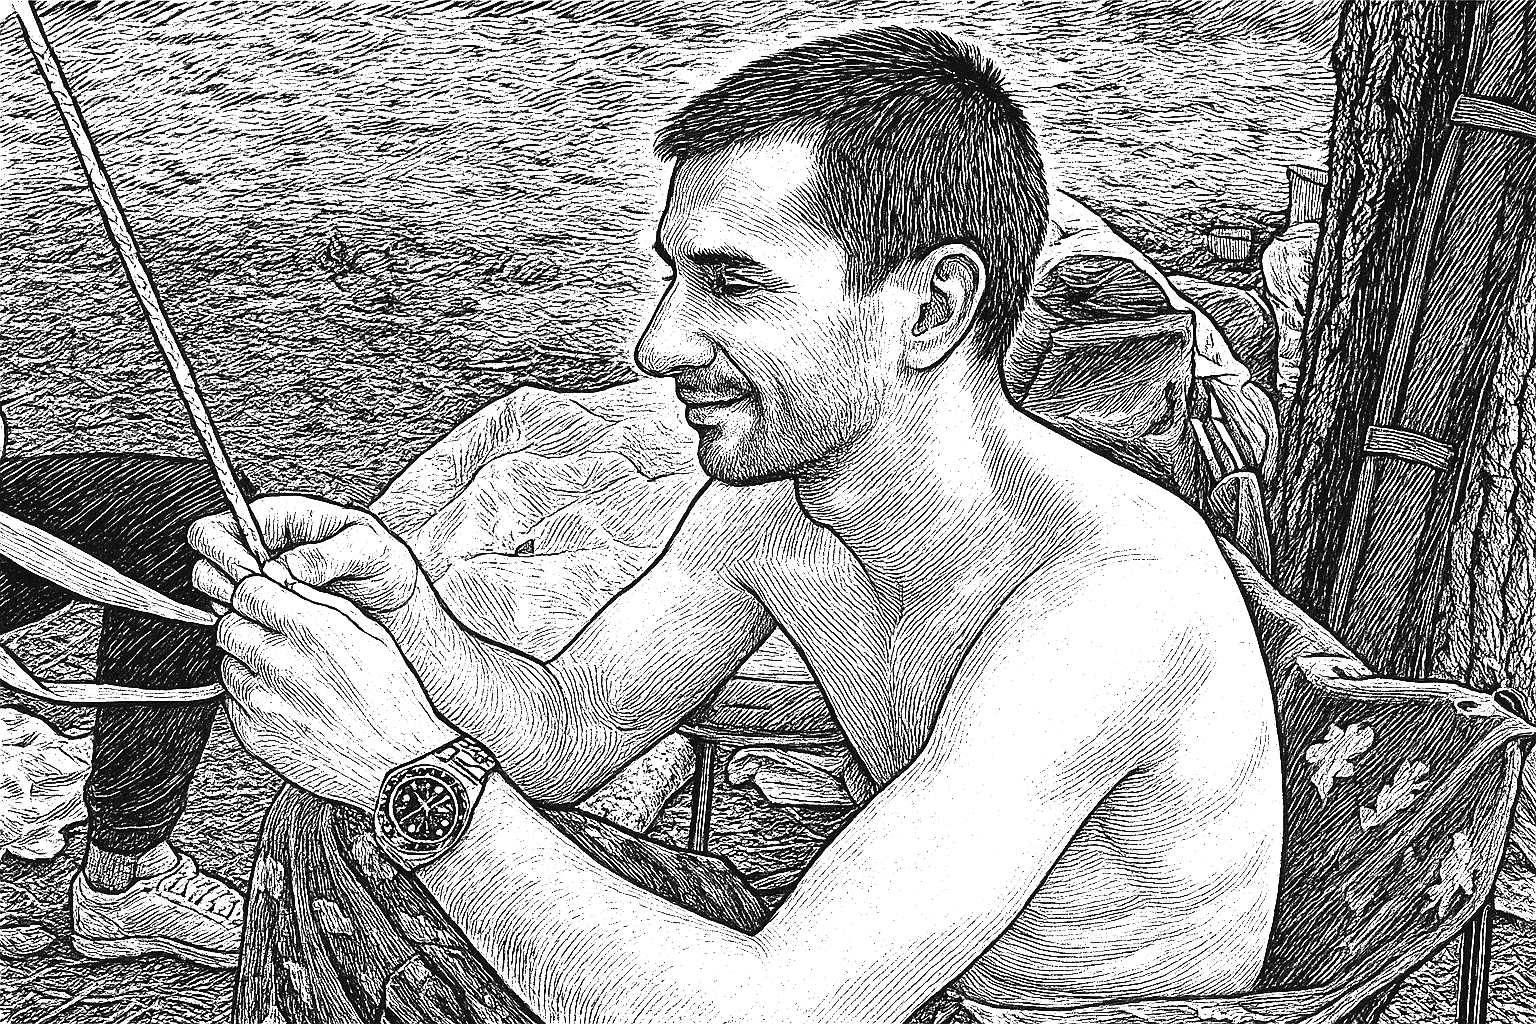
\includegraphics[width=1.0\textwidth]{28_1_chalka}
	\caption{\small\textit{...из этой ленты можно сплести чалку...}}
\end{figure}

%----------------------------------------------------------------
\newpage

\begin{figure}[h]
	\centering
	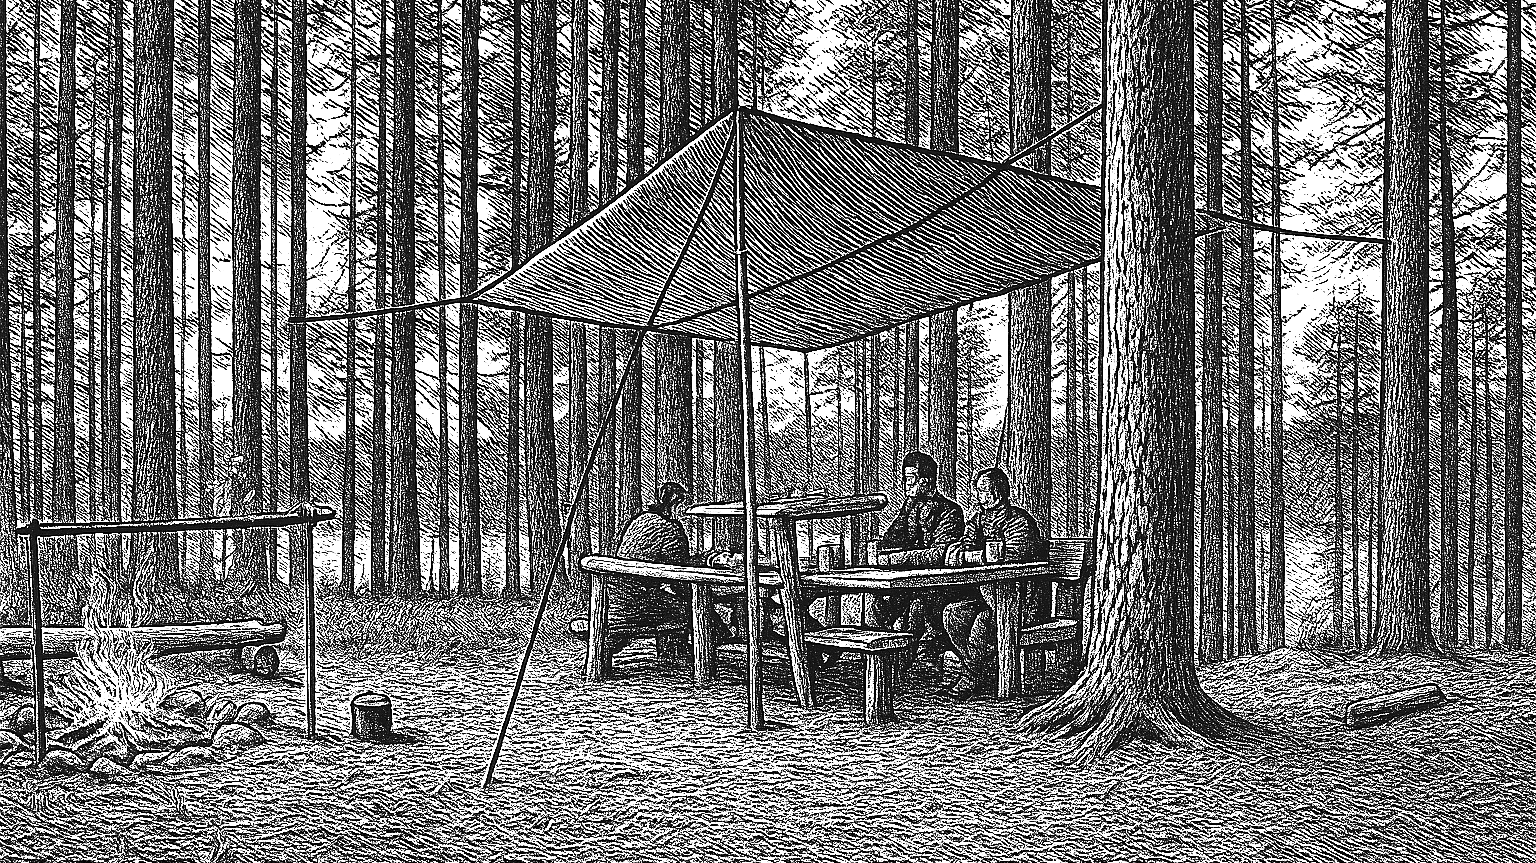
\includegraphics[width=1.0\textwidth]{29_1_tent}
	\caption{\small\textit{...в ослабший за ночь тент над~столом стала набираться вода...}}
\end{figure}

%----------------------------------------------------------------
\newpage

\begin{wrapfigure}[10]{r}{0.55\textwidth}
	%\begin{figure}[h]
	\centering
	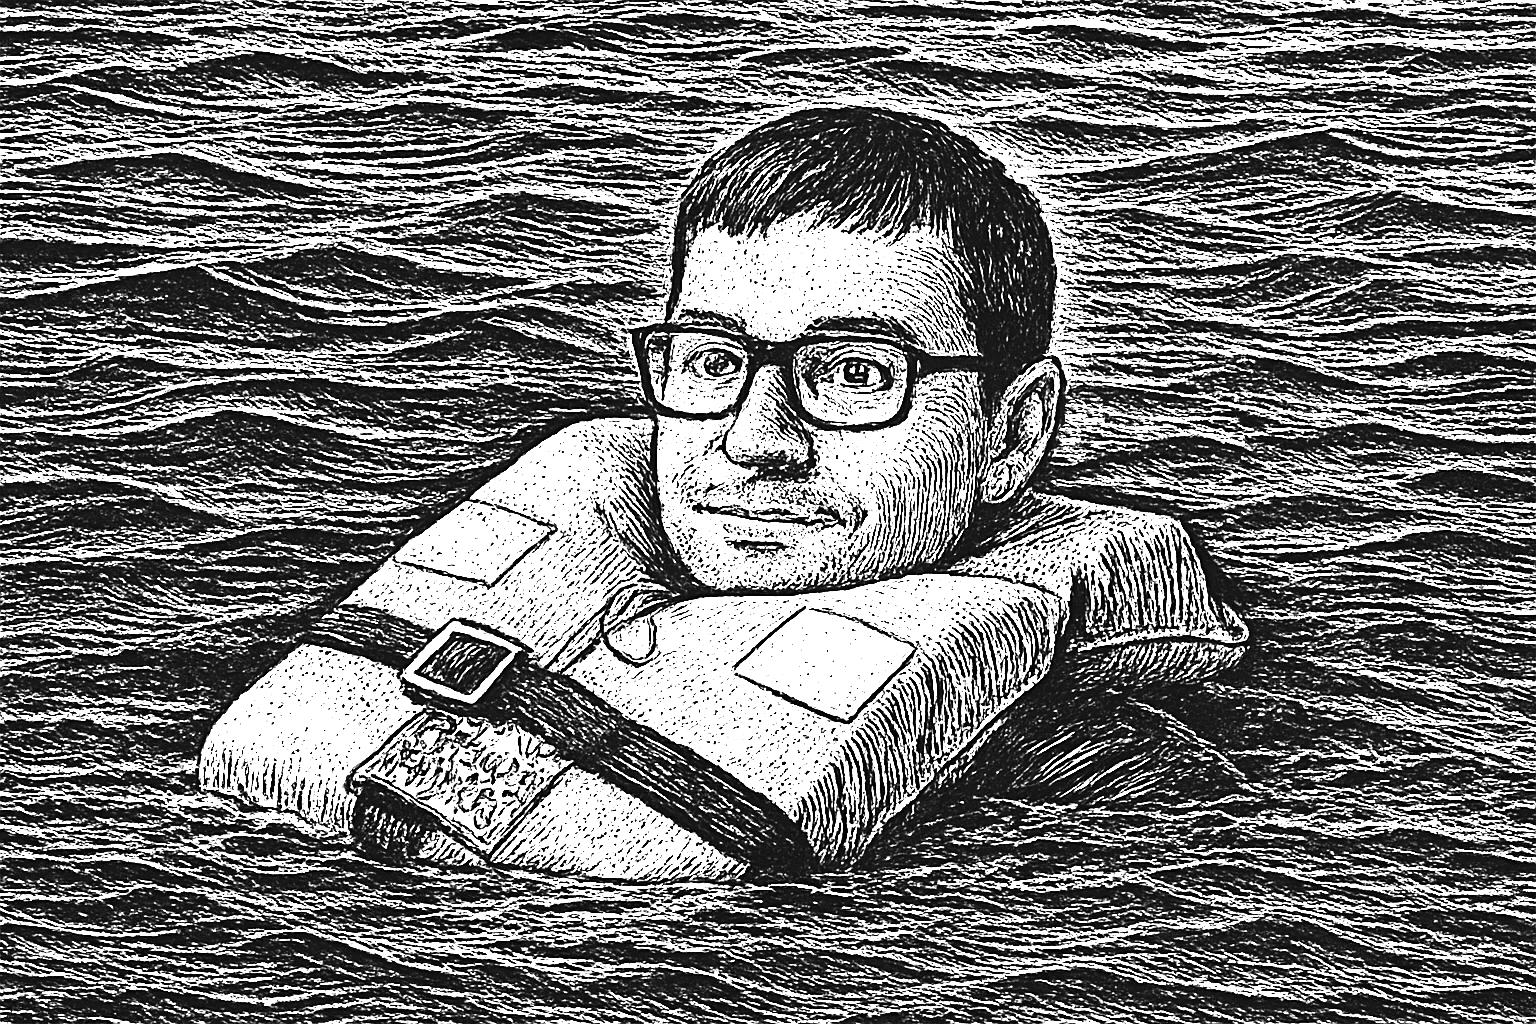
\includegraphics[width=0.5\textwidth]{30_1_lifejacket}
	\caption{\small\textit{...испытал свой спасжилет...}}
	%\end{figure}
\end{wrapfigure}испытал свой спасжилет и~успокоился. Руслан с~Пашей тусили под тентом, приканчивая красненькое:

\diagdash С бутылками что делать будем с пустыми? Не круто после себя стекло оставлять. Эх, молодо\sdash зелено, кто ж в~стекле с собой тащит?\mdash Паша разлил последнее.

%----------------------------------------------------------------
% 11 ГЛАВА
%----------------------------------------------------------------
\newpage

\begin{wrapfigure}[12]{l}{0.50\textwidth}
	%\begin{figure}[h]
	\centering
	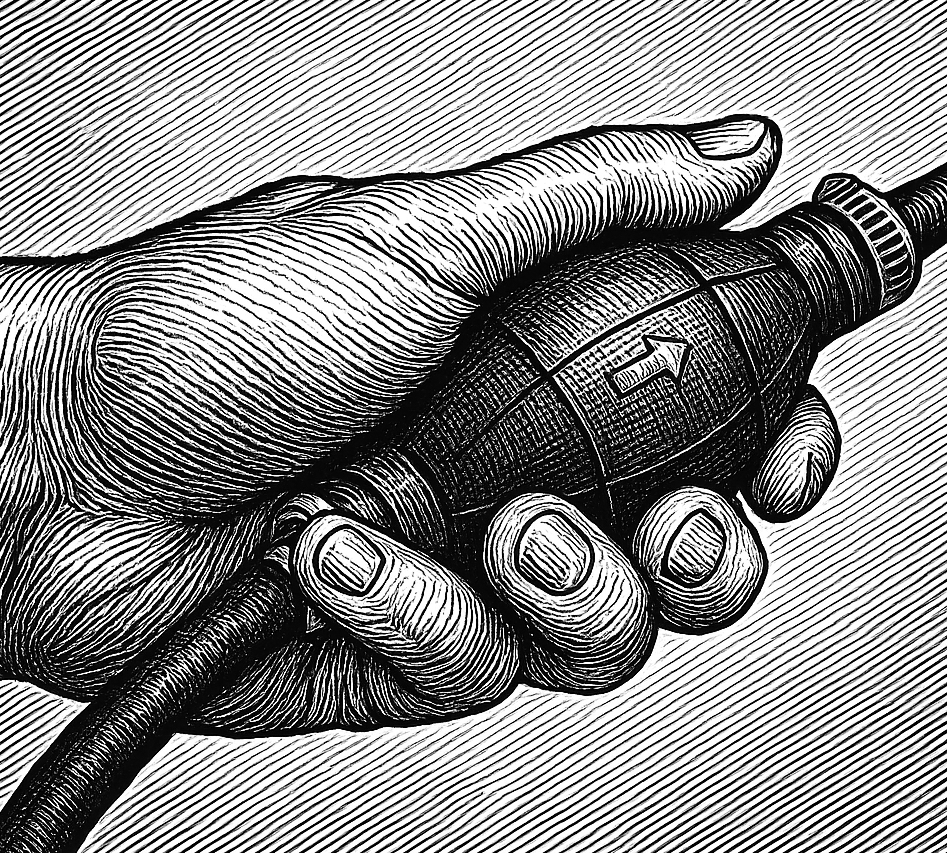
\includegraphics[width=0.5\textwidth]{31_pardon}
	\caption{\small\textit{...где моя, пардон...}}
	%\end{figure}
\end{wrapfigure}раз зажал и разжал грушу, отчего клапан в ней издал чавкающе\sdash булькающий звук.

\diagdash Ы-ы-ы! 

\diagdash Ну как\sdash то так, парни!\mdash Адмирал ещё раз проверил берег на~предмет забытых вещей и велел всем садиться в~байды.\mdash Пока мы собой и байдарочными юбками не~закроем проёмы, байды так и будет непрерывно заливать дождём!

%----------------------------------------------------------------
\newpage

\begin{figure}[h]
	\centering
	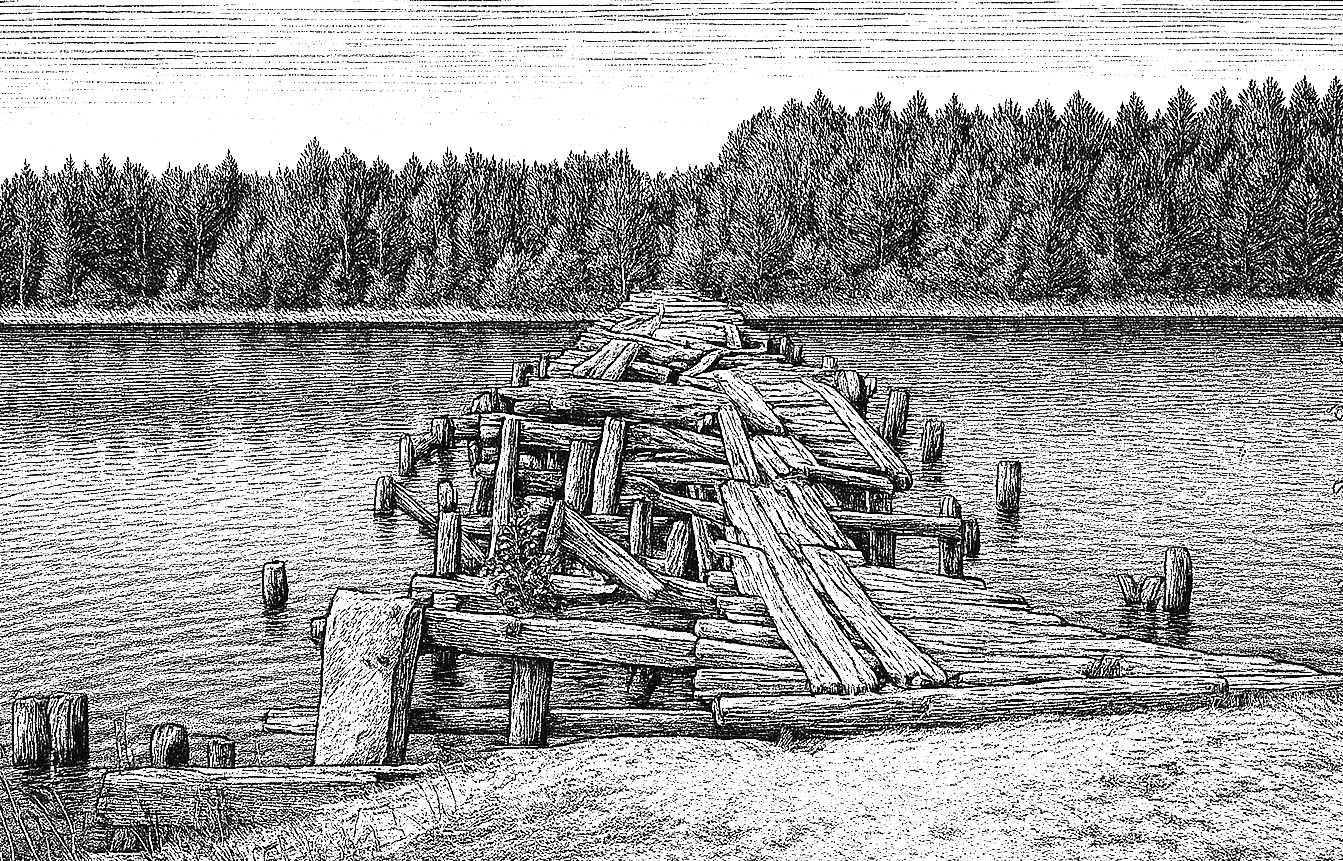
\includegraphics[width=1.0\textwidth]{32_1_bridge}
	\caption{\small\textit{...Вместо каких\sdash то пролётов лежало всего пару досок...}}
\end{figure}

%----------------------------------------------------------------
\newpage

\begin{figure}[h]
	\centering
	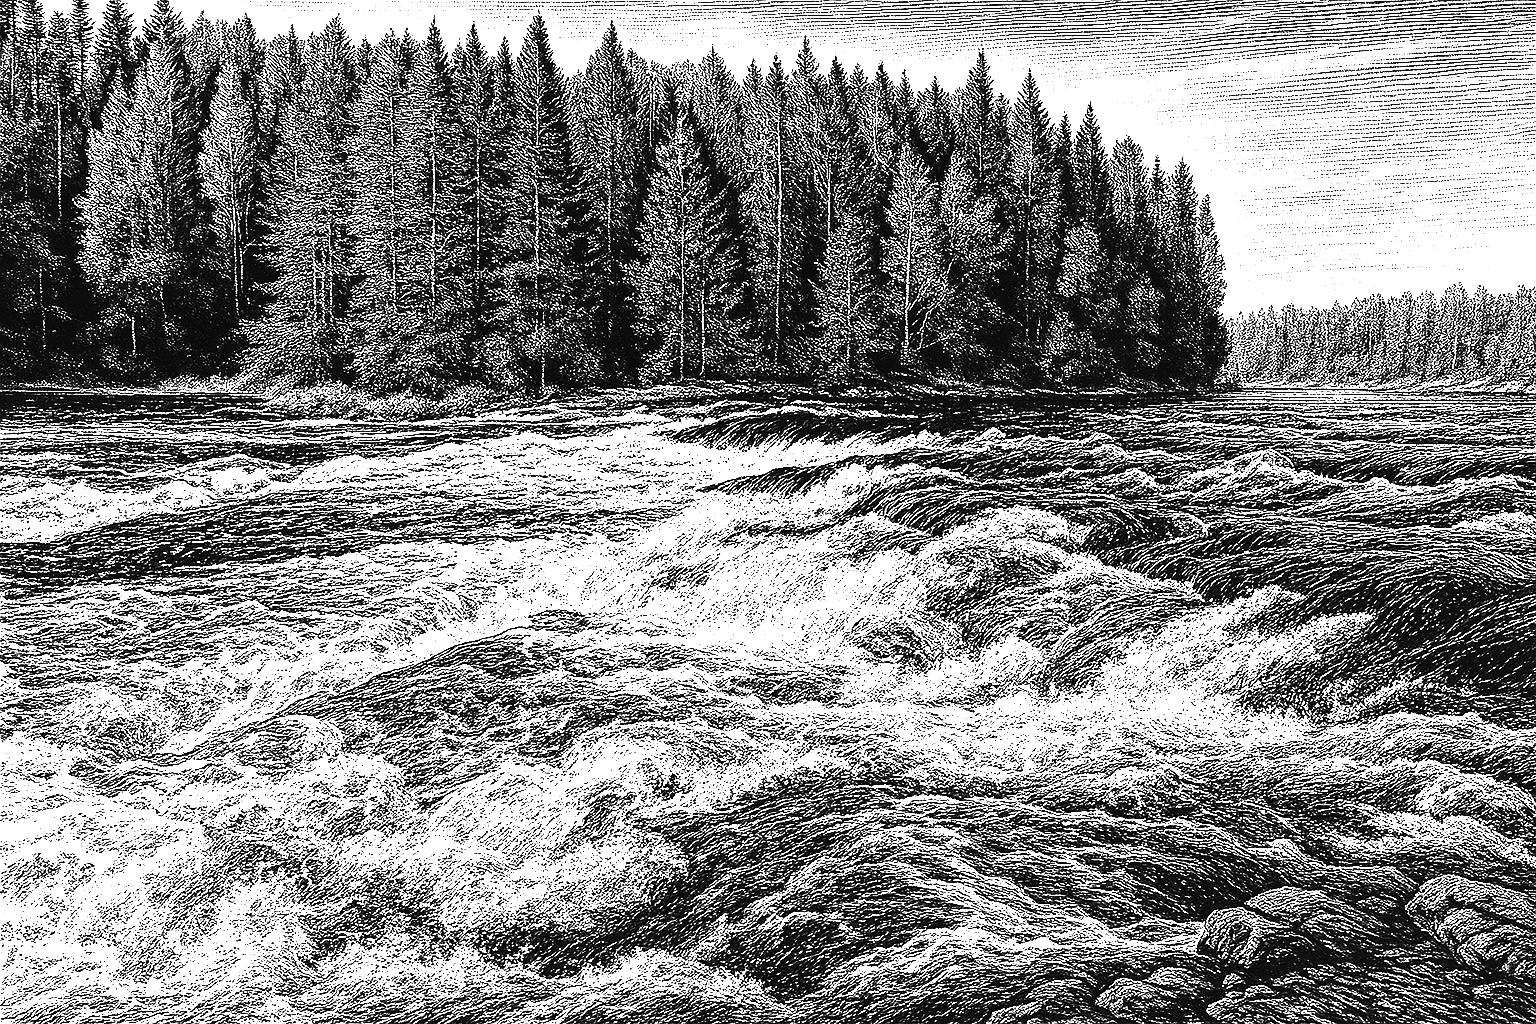
\includegraphics[width=1.0\textwidth]{33_1_porog}
	\caption{\small\textit{...Шум Уйтуженкоски...}}
\end{figure}

%----------------------------------------------------------------
\newpage

\begin{figure}[h]
	\centering
	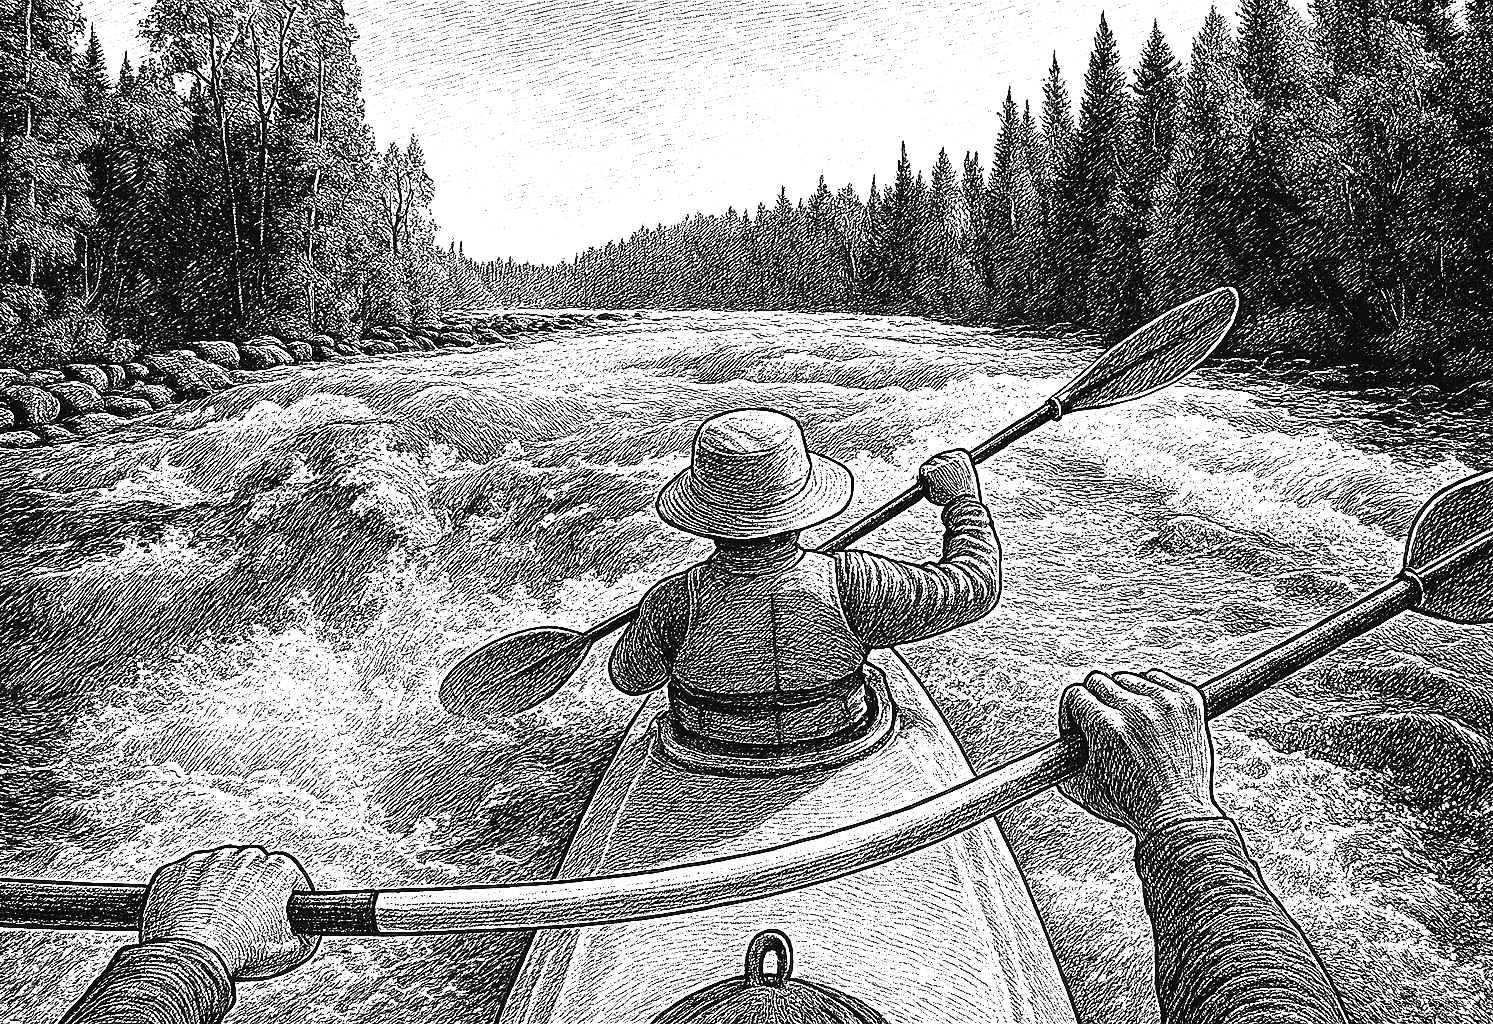
\includegraphics[width=1.0\textwidth]{34_1_shturm}
	\caption{\small\textit{...УПЁРЛИСЬ ЖЁСТКО ПО~ЛЕВОМУ!!!...}}
\end{figure}

%----------------------------------------------------------------
\newpage

\begin{figure}[h]
	\centering	
	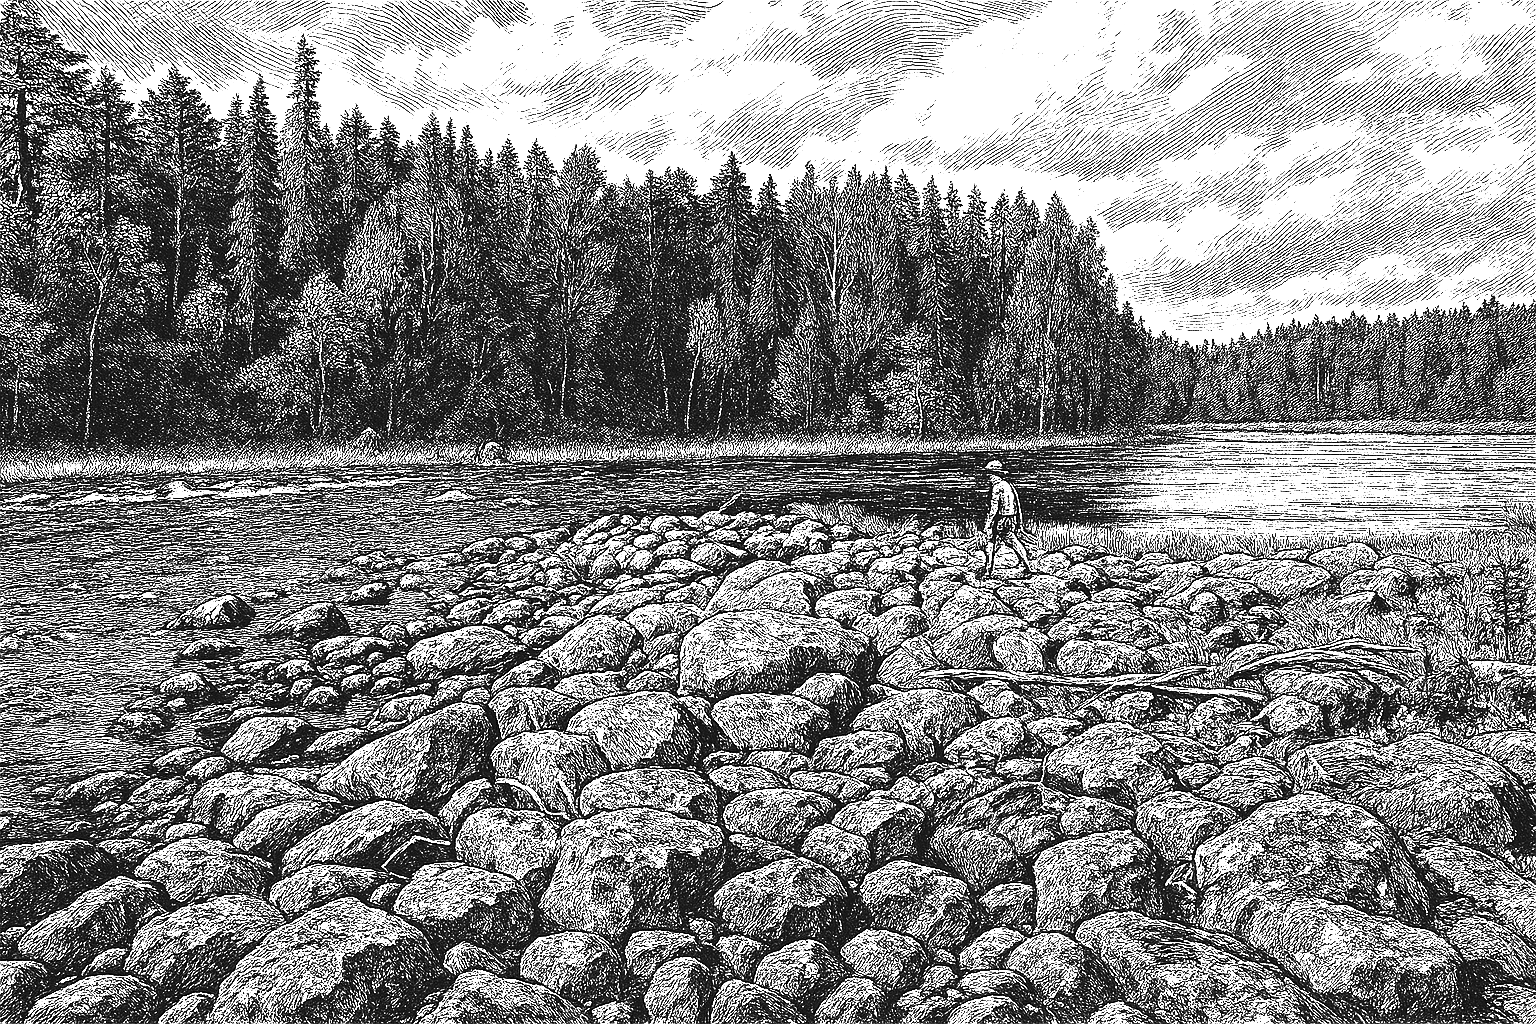
\includegraphics[width=1.0\textwidth]{35_1_otmel}
	\caption{\small\textit{...пошёл по каменистой гряде против течения...}}
\end{figure}

%----------------------------------------------------------------
\newpage

\begin{figure}[h]
	\centering
	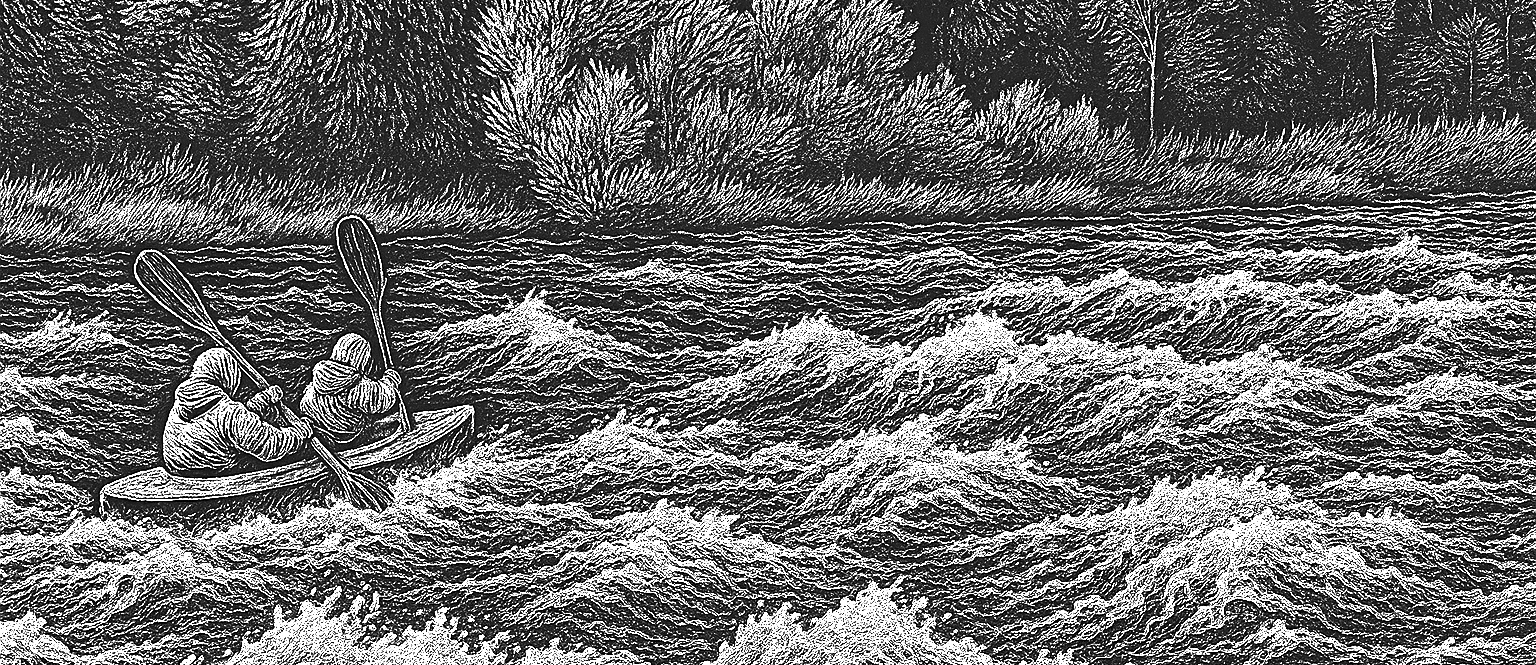
\includegraphics[width=1.0\textwidth]{36_3_zampolit}
	\caption{\small\textit{...Замполит как раз жёстко выгребал поворот...}}
\end{figure}

%----------------------------------------------------------------
\newpage

\begin{wrapfigure}[12]{r}{0.48\textwidth}
	%\begin{figure}[h]
	\centering
	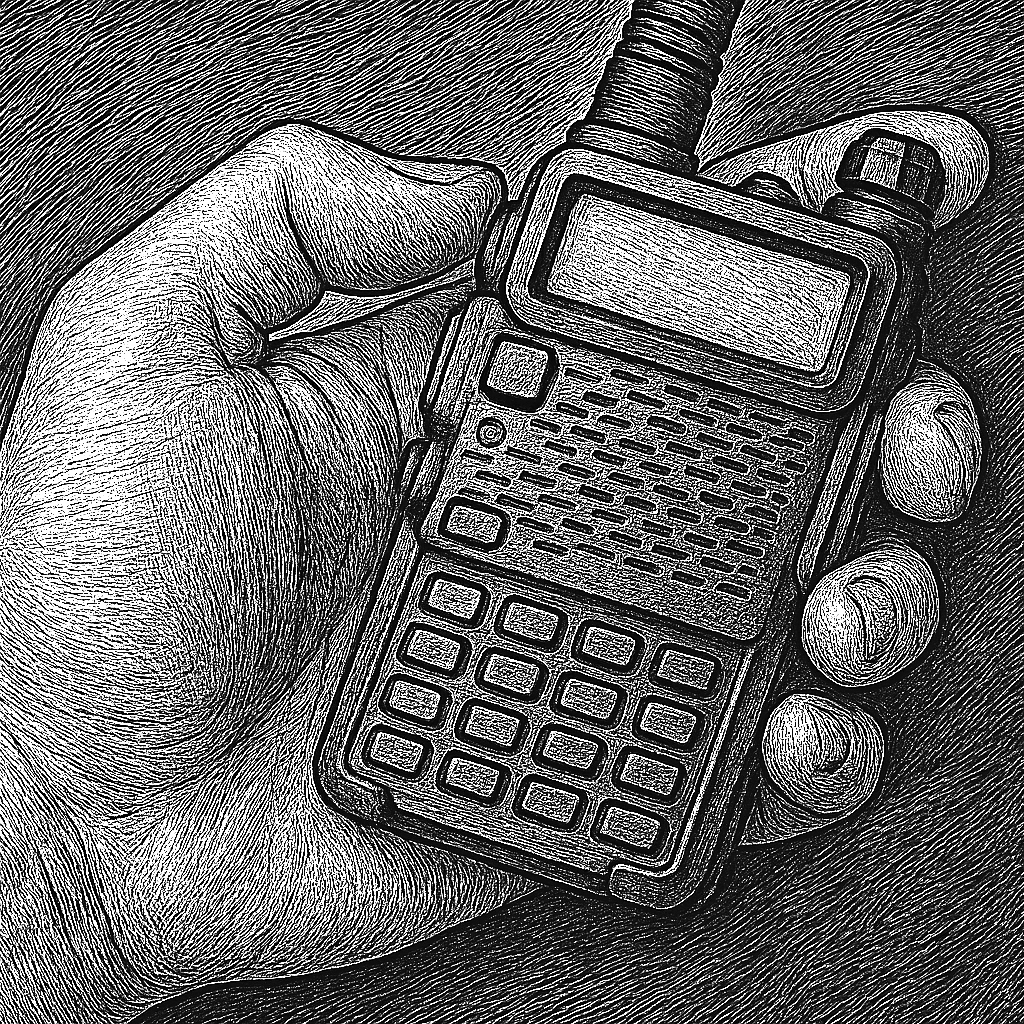
\includegraphics[width=0.46\textwidth]{37_1_radio}
	\caption{\small\textit{...спокуха, рация сдохла...}}
	%\end{figure}
\end{wrapfigure}

\diagdash Кнопку жмёшь и всё, экран гаснет, на.\mdash передал ему прибор Замполит.

\diagdash Ты её, засранец, позавчера не вырубил,\mdash догадался Адмирал.\mdash она у~тебя всю днёвку включённая была, сто процентов, вот аккумулятор и~сел в~ноль!!!

\diagdash Так ты не сказал$\ldots$

Адмирал уже набрал полные лёгкие разразиться матерной тирадой, но~удержался и только сказал, выдохнув:

%----------------------------------------------------------------
\newpage

\begin{figure}[h]
	\centering
	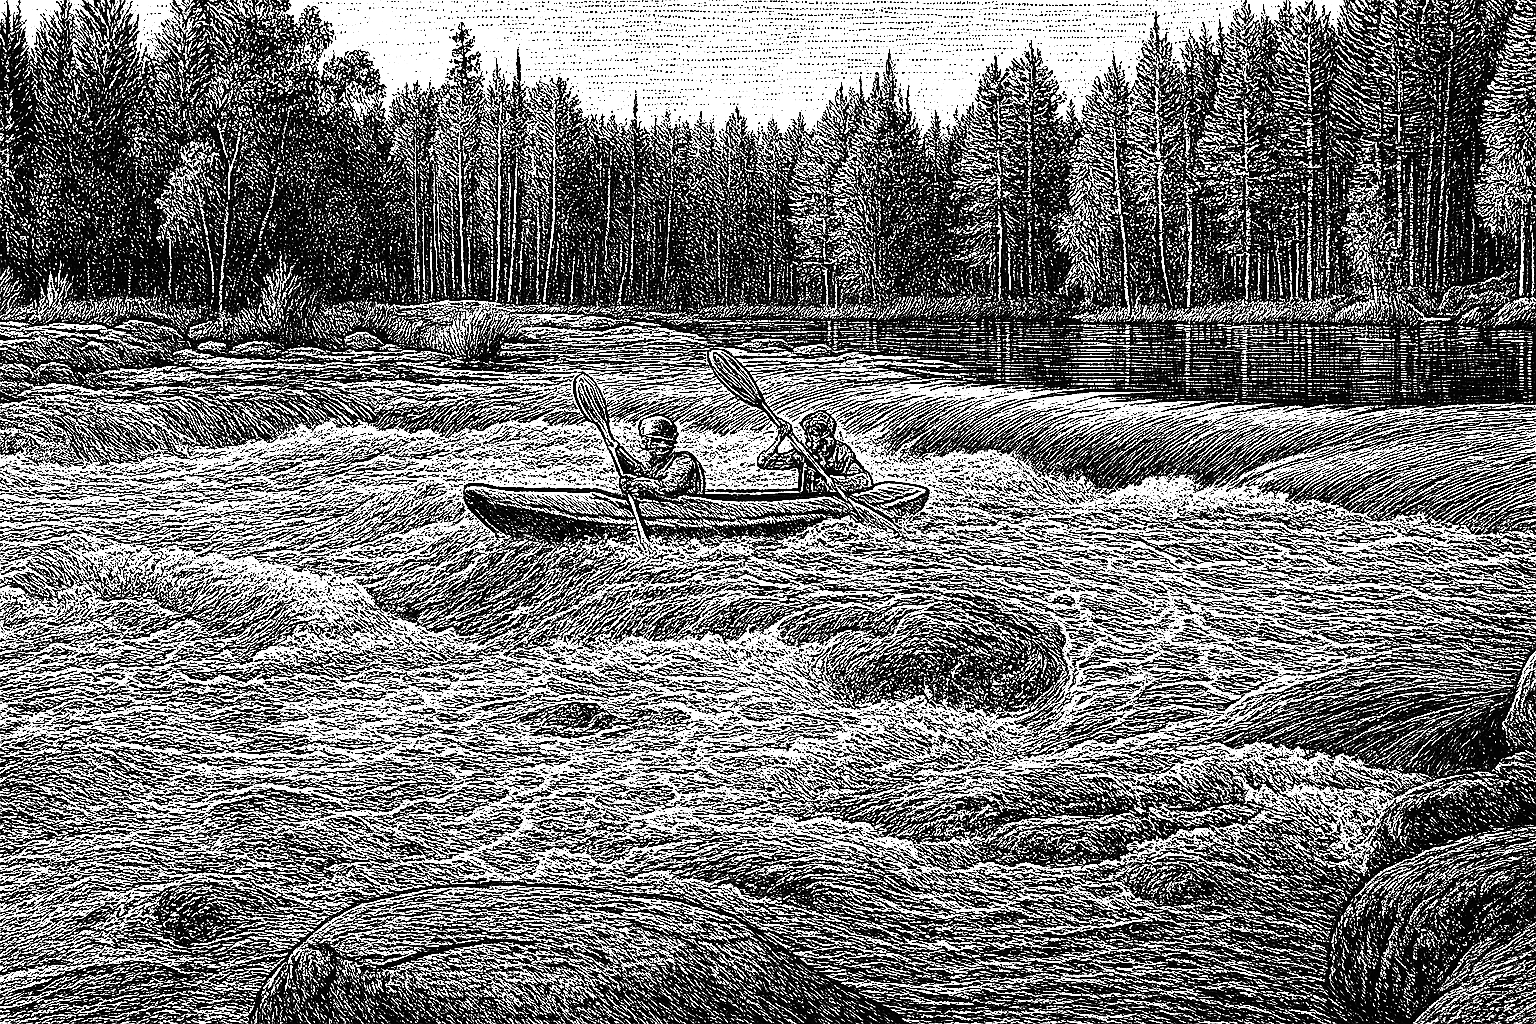
\includegraphics[width=1.0\textwidth]{38_1_suhoi}
	\caption{\small\textit{...ребята увидали выход из~порога...}}
\end{figure}

%----------------------------------------------------------------
\newpage

\begin{wrapfigure}[17]{r}{0.5\textwidth}
	%\begin{figure}[h]
	\centering
	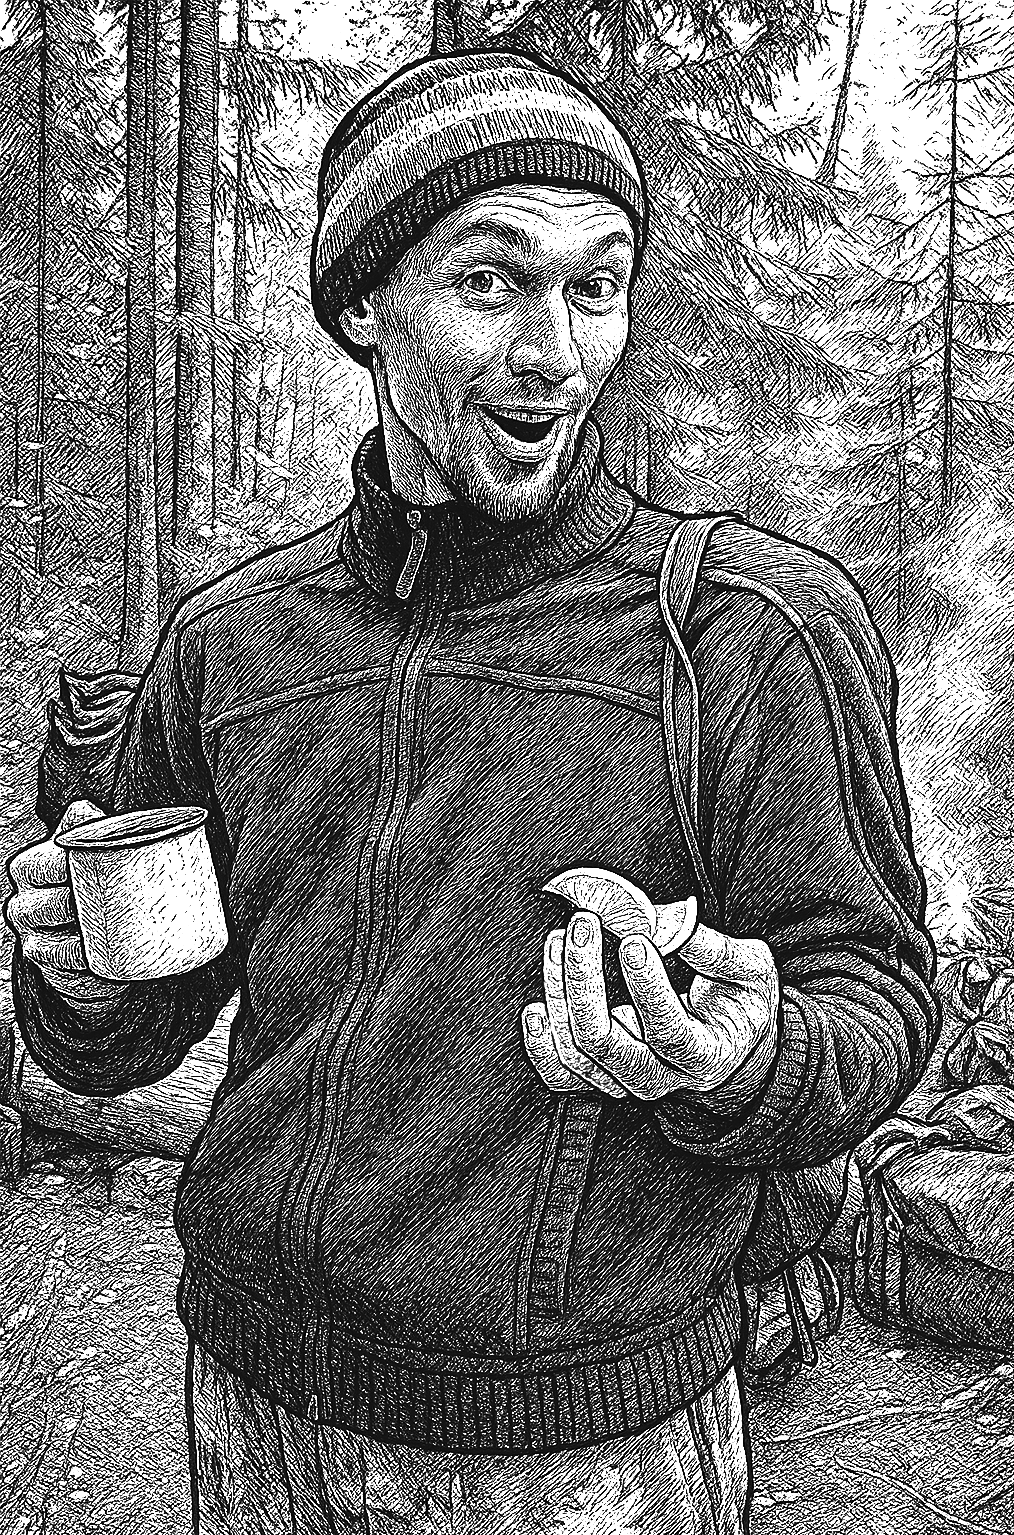
\includegraphics[width=0.46\textwidth]{39_2_rum}
	\caption{\small\textit{...чай, лимон, всё харашо!...}}
	%\end{figure}
\end{wrapfigure}
\diagdash Можно уже, да?

\diagdash А то!

\diagdash Итак, мужики!\mdash начал Адмирал, пародируя акцент.\mdash Там шумит порог Каданлоама! Мы стоим тут на~островэ! У нас есть$\ldots$\mdash он посмотрел в кружку, полную кубинского рома,\mdash $\ldots$чай, лимон, всё харашо! Да? Мы~переоделись в сухоэ, одэжда у нас вон там на вэрёвочке сушится висит! Кирь, засними эту выставку\sdash продажу! Вон~там всё сушится!$\ldots$


\diagdash После героического прохождения порогов!\mdash вставил Паша.

%----------------------------------------------------------------
\newpage

\begin{figure}[h]
	\centering
	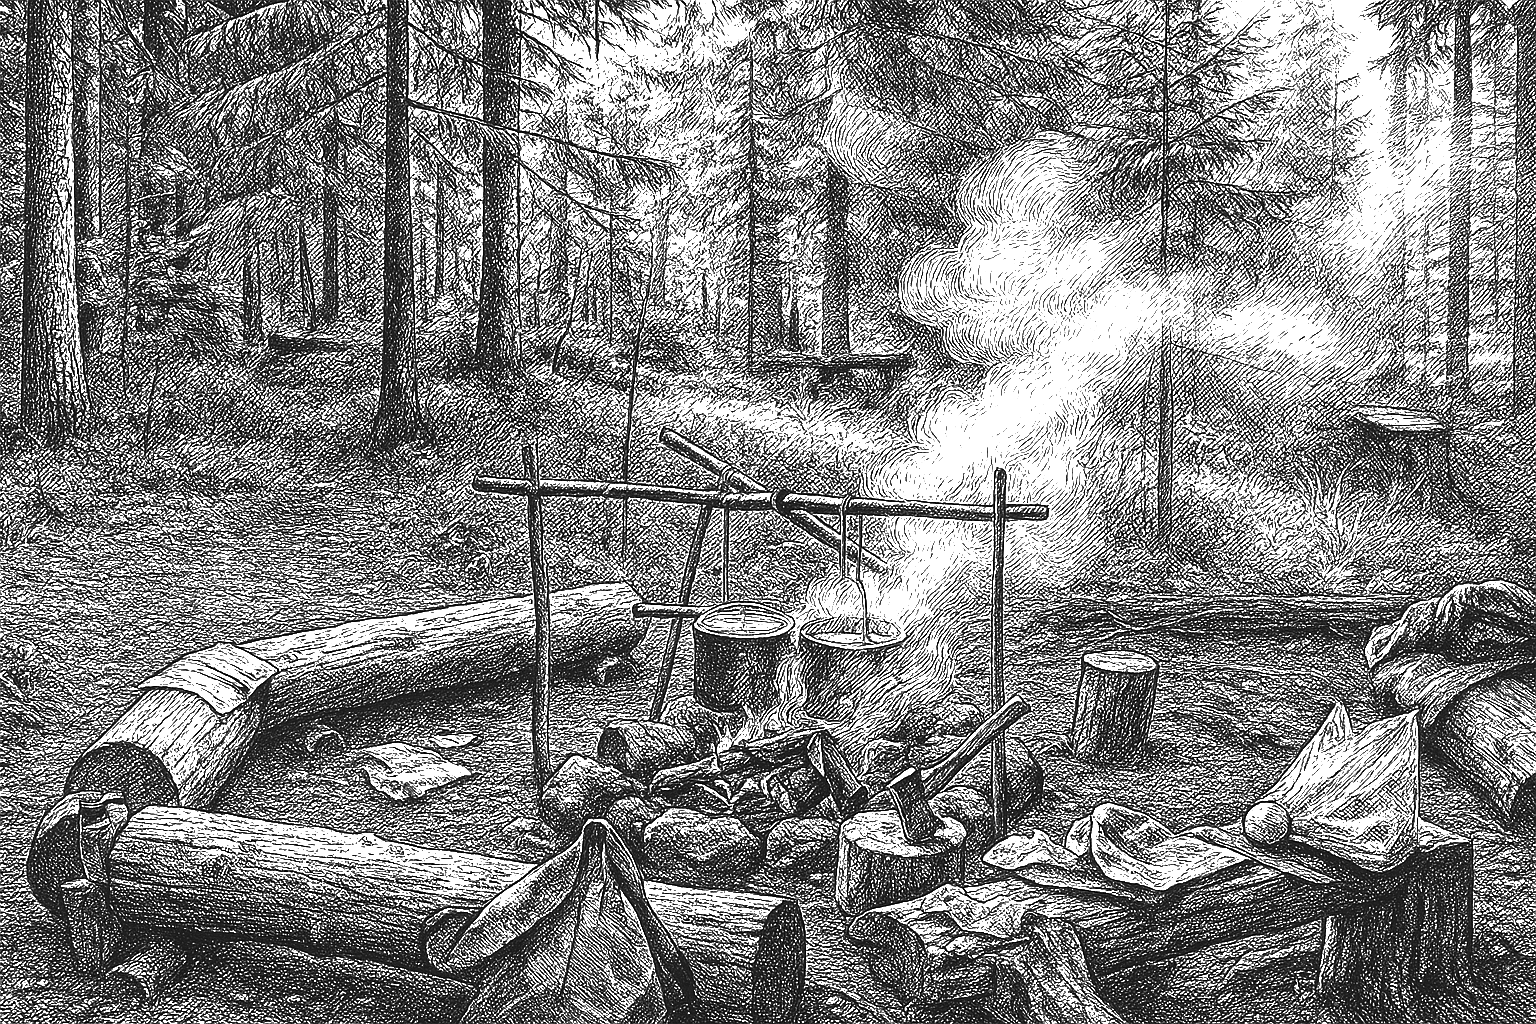
\includegraphics[width=1.0\textwidth]{40_1_fire}
	\caption{\small\textit{...у пылающего костра...}}
\end{figure}


%----------------------------------------------------------------
\newpage

\begin{figure}[h]
	\centering
	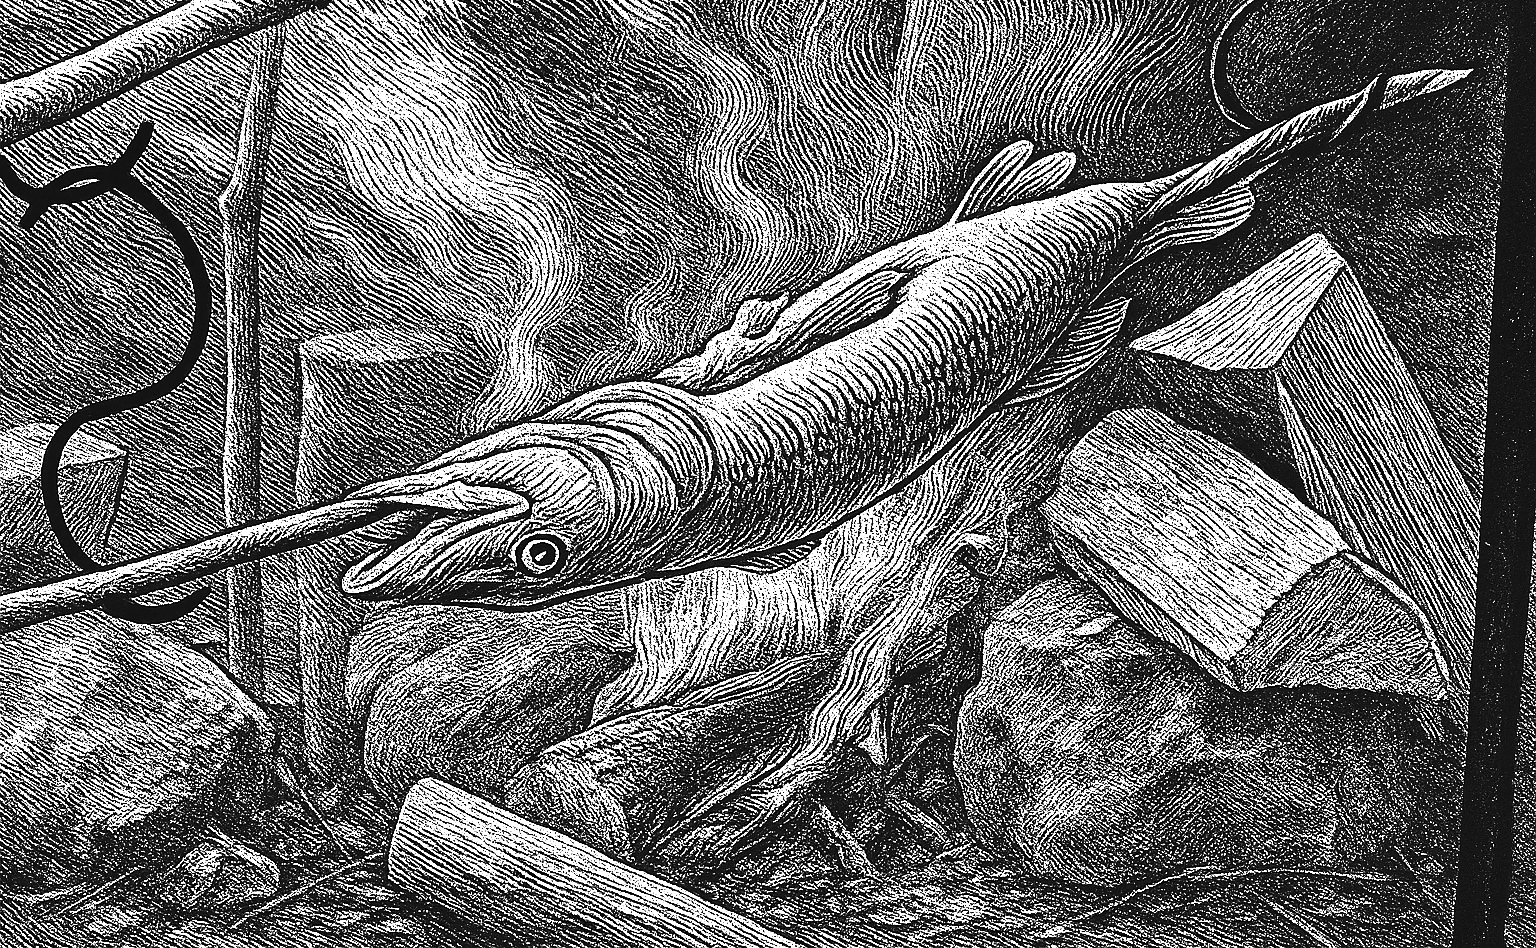
\includegraphics[width=1.0\textwidth]{41_1_pikefish}
	\caption{\small\textit{...ещё и щука под вечер...}}
\end{figure}

%----------------------------------------------------------------
\newpage

\begin{figure}[h]
	\centering
	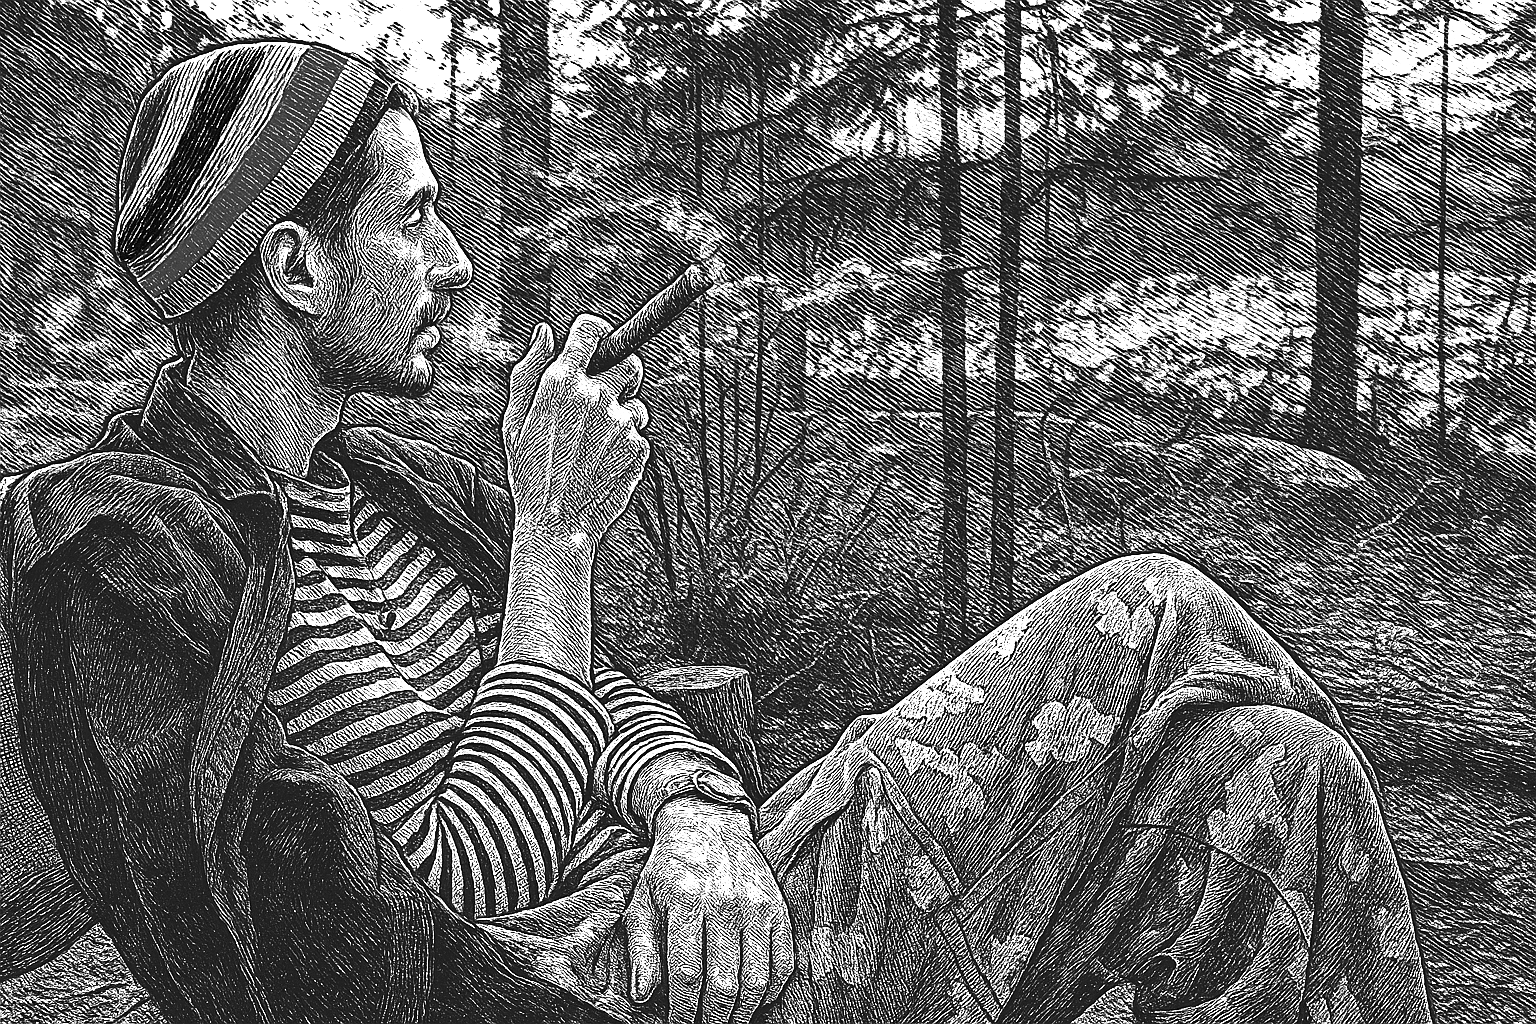
\includegraphics[width=1.0\textwidth]{42_3_cigar}
	\caption{\small\textit{...вечер проходил у них с ленцой...}}
\end{figure}

%----------------------------------------------------------------
\newpage

\begin{figure}[h]
	\centering
	%	\includegraphics[width=1.0\textwidth]{11_5}
	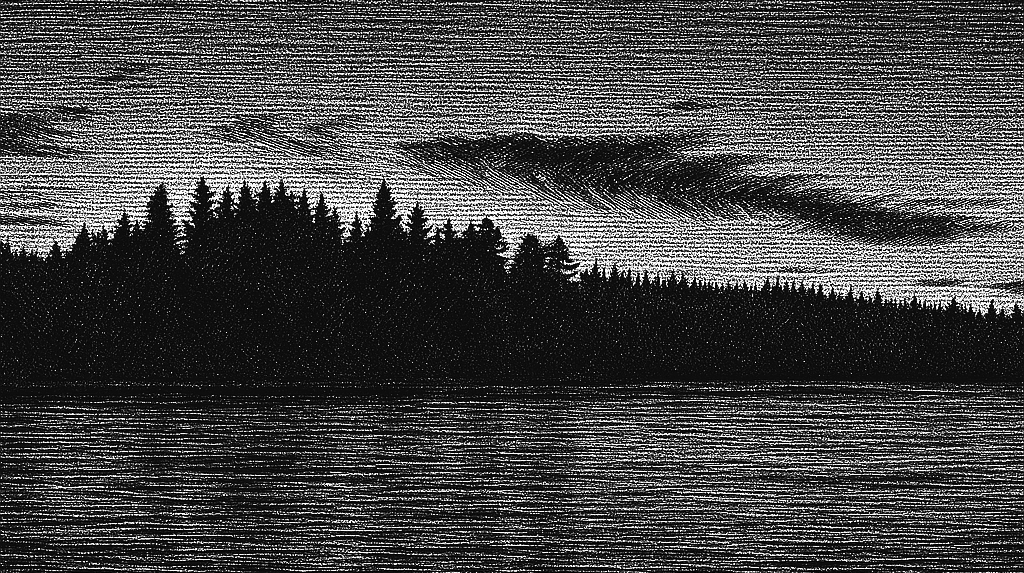
\includegraphics[width=1.0\textwidth]{43_1_cheranga}
	\caption{\small\textit{...Адмирал сходил к берегу пофотографировать разлив Черанги...}}
\end{figure}

%----------------------------------------------------------------
% 12 ГЛАВА
%----------------------------------------------------------------
\newpage

\begin{wrapfigure}[12]{l}{0.48\textwidth}
	%\begin{figure}[h]
	\centering
	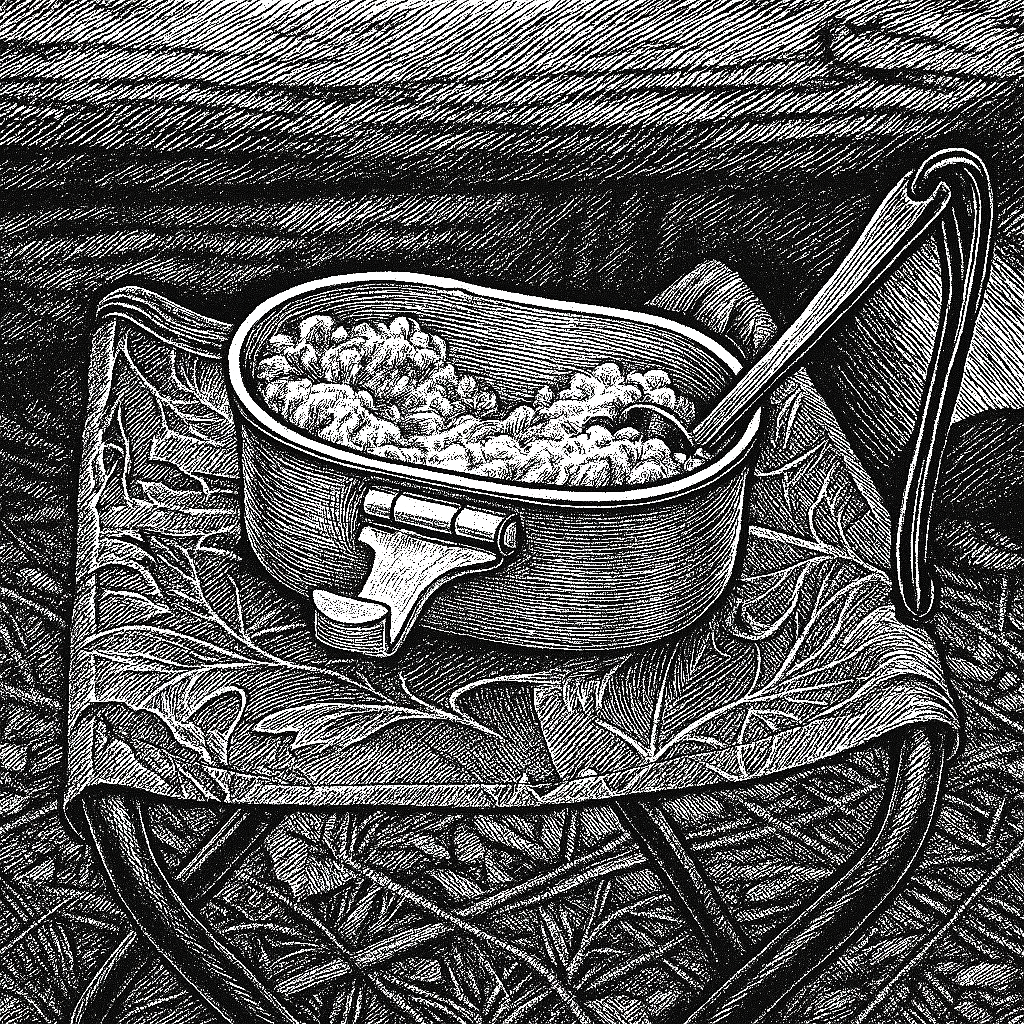
\includegraphics[width=0.45\textwidth]{44_1_porridge}
	\caption{\small\textit{...пшёнка с изюмом...}}
	%\end{figure}
\end{wrapfigure}
\diagdash Сань, чё у нас сегодня?\mdash Паша покончил с~кашей и~достал конфеты к~чаю.

\diagdash Вчера обсуждали вродь как. Сегодня\mdash ещё 4 порога последних и дальше по широкой Суне почти до~Викшозера. Кирь, доставай описание порогов\mdash самое время освежить в~памяти.
%----------------------------------------------------------------
\newpage

\begin{figure}[h]
	\centering
	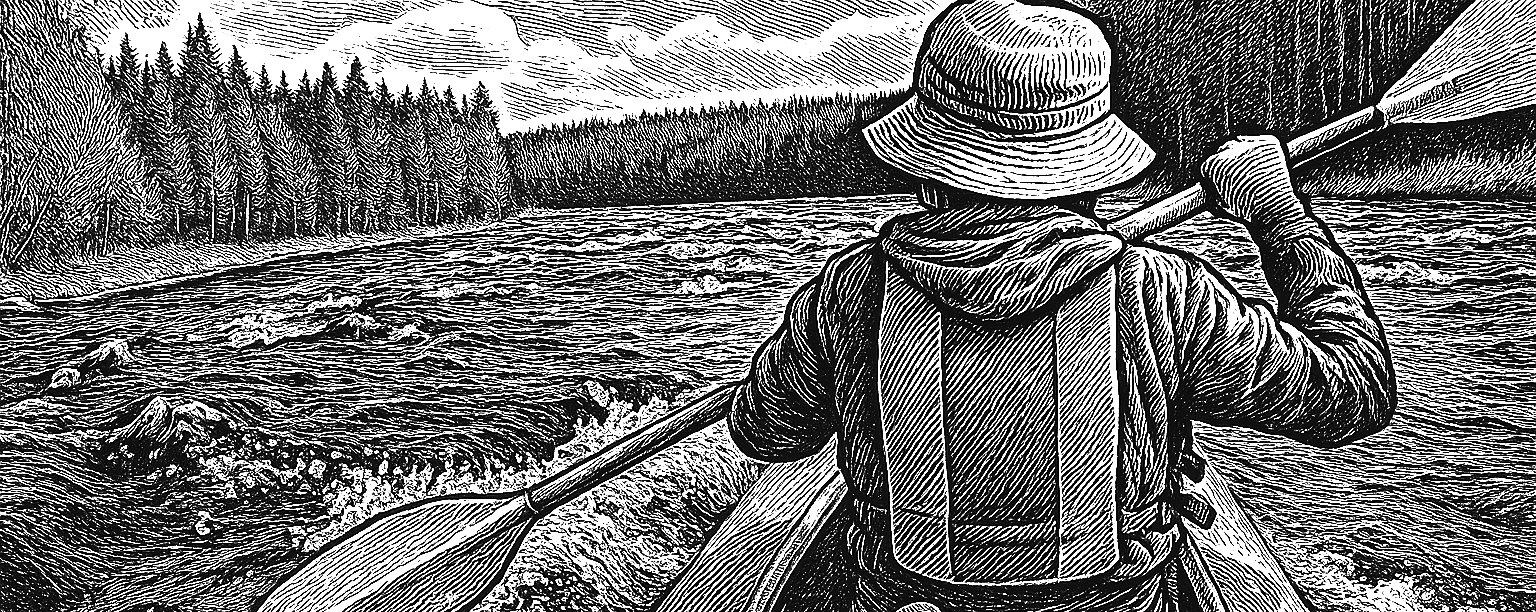
\includegraphics[width=1.0\textwidth]{45_1_bochka}
	\caption{\small\textit{...рубанули байдаркой прямо по плите...}}
\end{figure}

%----------------------------------------------------------------
\newpage

\begin{figure}[h]
	\centering
	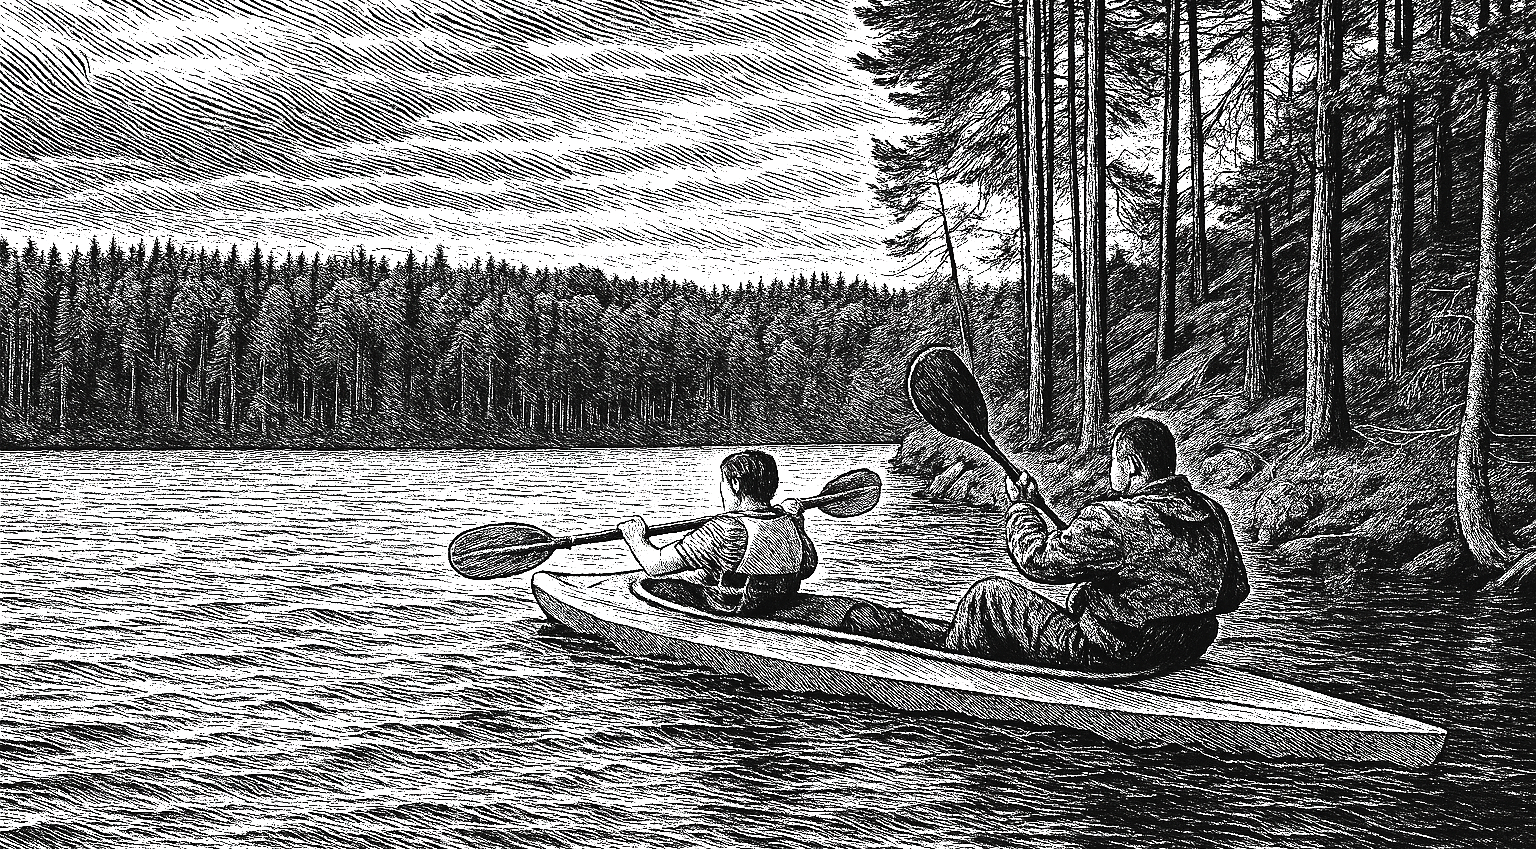
\includegraphics[width=1.0\textwidth]{46_1_endporogs}
	\caption{\small\textit{...пороги кончились...}}
\end{figure}

%----------------------------------------------------------------
% 13 ГЛАВА
%----------------------------------------------------------------
\newpage

\begin{wrapfigure}[13]{l}{0.5\textwidth}
	%\begin{figure}[h]
	\centering
	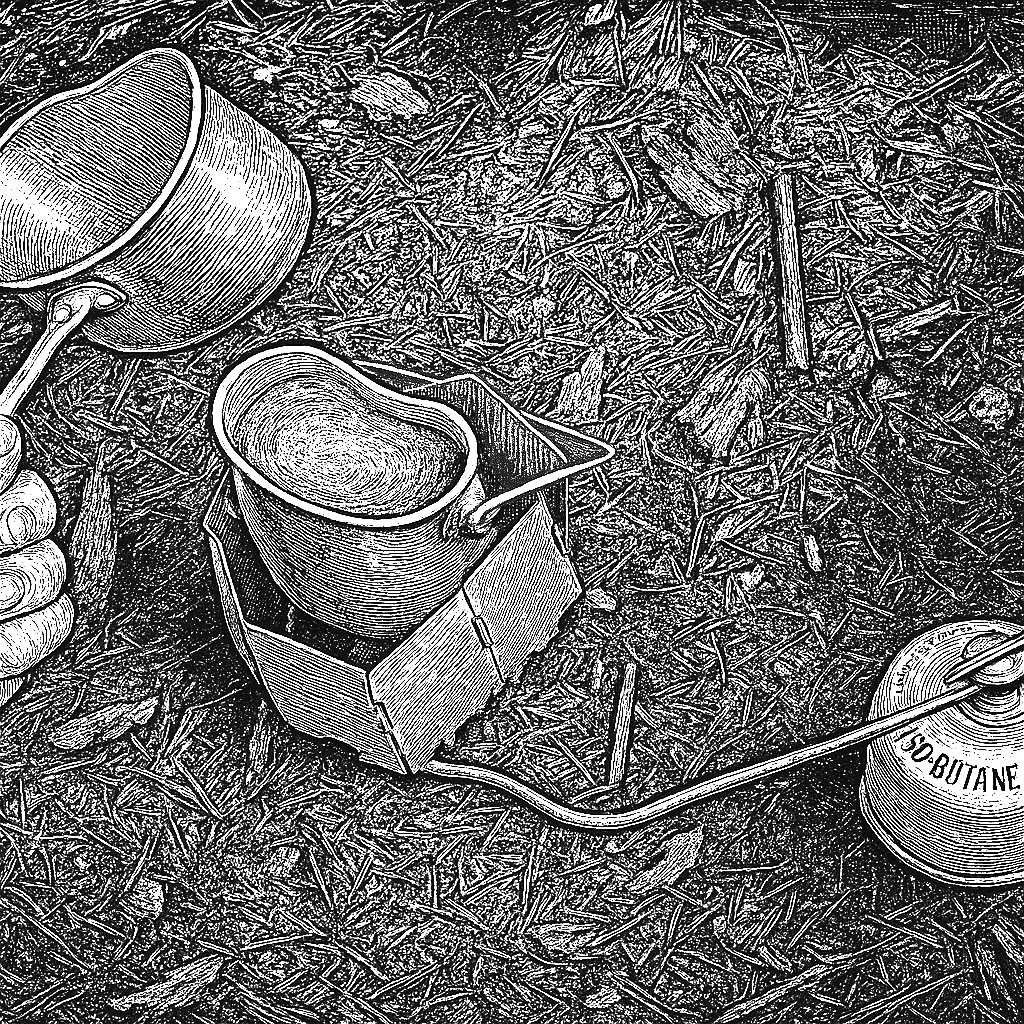
\includegraphics[width=0.47\textwidth]{47_1_coffee}
	\caption{\small\textit{...я вам кофеёк обещал...}}
	%\end{figure}
\end{wrapfigure}
Адмирал выполз из~палатки. Дождь почти закончился, но~погодка оставляла желать лучшего\mdash лес вокруг был влажным, дул неслабый ветерочек. Он~распалил костёр из~напиленных вчера впрок дров, поставил воду в~котелке на~чай\mdash всё равно кто\sdash нибудь да захочет чай\mdash и~принялся за кофе. Немного подумав, решил варить кофе на~газу, а~не~на~костре. Для этого он достал и собрал свою мини\sdash горелку, собрал защитный экранчик от ветра, поставил десантный котелок на синий цветок газа, щедро насыпал молотый кофе. Сверху он закрыл котелок подкотельником\mdash получилась как бы крышка\mdash так быстрее закипело. Народ потихонку стал подтягиваться к костру.

%----------------------------------------------------------------
\newpage

\begin{wrapfigure}[20]{r}{0.58\textwidth}
	%\begin{figure}[h]
	\centering
	\includegraphics[width=0.56\textwidth]{48_1_pancakes}
	\caption{\small\textit{...принялся за оладьи...}}
	%\end{figure}
\end{wrapfigure}
\diagdash Шурик, такого ты ещё не делал.\mdash изрёк подошедший Замполит, тоже соблазнившись на~кофе.

\diagdash Не, помнишь, мы когда в последний раз по Чагодоще ходили, тоже кофеёк варили как\sdash то?

\diagdash А, тот наш <<арктический>> поход? Смутно~уже.

\diagdash Варили\sdash варили, было дело.\mdash подтвердил Серёга.

\diagdash Ну вот я решил повторить, так сказать.\mdash Адмирал вполне насладился напитком и принялся за оладьи. Он~достал из продуктовой гермы блинную муку и стал читать инструкцию на упаковке.


%----------------------------------------------------------------
\newpage

\begin{wrapfigure}[10]{r}{0.5\textwidth}
	%\begin{figure}[h]
	\centering
	\includegraphics[width=0.48\textwidth]{49_1_kompot}
	\caption{\small\textit{...компотика наварить?...}}
	%\end{figure}
\end{wrapfigure}

Спустя совсем немного времени компот был готов:

\diagdash Нава-а-аристо!

\diagdash А то!

\diagdash Серёга у нас главный по компотам в~этом сплаве.\mdash попробовал компот Руслан.

\diagdash Не, по компотикам главный\mdash Замполит, а Серёга по сборке голубики.\mdash не преминул подколоть Замполита Адмирал.

%----------------------------------------------------------------
\newpage

\begin{wrapfigure}[22]{l}{0.58\textwidth}
	%\begin{figure}[h]
	\centering
	\includegraphics[width=0.56\textwidth]{50_1_fishsmoke}
	\caption{\small\textit{...Паша стал снимать рыбу...}}
	%\end{figure}
\end{wrapfigure}
ываооывшоа ываы ывщшао ывашгор ываг вргш ывар вышгфр рывы горгшр ш щш щш шщг щшгщшг  гшны ы ываооывшоа ываы ывщшао ывашгор ываг вргш ывар вышгфр рывы горгшр ш щш щш шщг щшгщшг  гшны ы ываооывшоа ываы ывщшао ывашгор ываг вргш ывар вышгфр рывы горгшр ш щш щш шщг щшгщшг  гшны ы ываооывшоа ываы ывщшао ывашгор ываг вргш ывар вышгфр рывы горгшр ш щш щш шщг щшгщшг  гшны ы ываооывшоа ываы ывщшао ывашгор ываг вргш ывар вышгфр рывы горгшр ш щш щш шщг щшгщшг  гшны ы ываооывшоа ываы ывщшао ывашгор ываг вргш ывар вышгфр рывы горгшр ш щш щш шщг щшгщшг  гшны ы ываооывшоа ываы ывщшао ывашгор ываг вргш ывар вышгфр рывы горгшр 

ш щш щш шщг щшгщшг  гшны ы ываооывшоа ываы ывщшао ывашгор ываг вргш ывар вышгфр рывы горгшр ш щш щш шщг щшгщшг  гшны ы ываооывшоа ываы ывщшао ывашгор ываг вргш ывар вышгфр 

%----------------------------------------------------------------
\newpage

\begin{wrapfigure}[11]{l}{0.58\textwidth}
	%\begin{figure}[h]
	\centering
	\includegraphics[width=0.56\textwidth]{51_1_mushrooms}
	\caption{\small\textit{...зажарили лисички...}}
	%\end{figure}
\end{wrapfigure}
ывар вышгфр рывы горгшр ш щш щш шщг щшгщшг  гшны ы ываооывшоа ываы ывщшао ывашгор ываг вргш ывар вышгфр рывы горгшр ш щш щш шщг щшгщшг  гшны ы ываооывшоа ываы ывщшао ывашгор ываг вргш ывар вышгфр рывы горгшр ш щш щш шщг щшгщшг  гшны ы ываооывшоа ываы ывщшао 

ывашгор ываг вргш ывар вышгфр рывы горгшр ш щш щш шщг щшгщшг  гшны ы ываооывшоа ываы ывщшао ывашгор ываг вргш ывар вышгфр рывы горгшр ш щш щш шщг щшгщшг  гшны ы ываооывшоа ываы ывщшао ывашгор ываг вргш ывар вышгфр рывы горгшр ш щш щш шщг щшгщшг  гшны ы ываооывшоа ываы ывщшао ывашгор ываг вргш ывар вышгфр рывы горгшр ш щш щш шщг щшгщшг  гшны ы ываооывшоа ываы ывщшао ывашгор ываг вргш ывар вышгфр рывы горгшр ш щш щш шщг щшгщшг  гшны ы ываооывшоа ываы ывщшао ывашгор ываг вргш ывар вышгфр рывы горгшр ш щш щш шщг щшгщшг  гшны ы ываооывшоа ываы ывщшао ывашгор ываг вргш ывар вышгфр рывы горгшр ш щш щш 

%----------------------------------------------------------------
\newpage

\begin{wrapfigure}[12]{l}{0.58\textwidth}
	%\begin{figure}[h]
	\centering
	\includegraphics[width=0.56\textwidth]{52_1_delight}
	\caption{\small\textit{...Адмирал закрыл глаза...}}
	%\end{figure}
\end{wrapfigure}
шщг щшгщшг  гшны ы ываооывшоа ываы ывщшао ывашгор ываг вргш ывар вышгфр рывы горгшр ш щш щш шщг щшгщшг  гшны ы ываооывшоа ываы ывщшао ывашгор ываг вргш ывар вышгфр рывы горгшр ш щш щш шщг щшгщшг  гшны ы ываооывшоа ываы ывщшао ывашгор ываг вргш ывар вышгфр рывы горгшр ш щш щш шщг щшгщшг  гшны ы ываооывшоа ываы ывщшао ывашгор ываг вргш ывар вышгфр рывы горгшр ш щш щш шщг щшгщшг  гшны ы ываооывшоа ываы ывщшао ывашгор ываг вргш ывар вышгфр рывы горгшр ш щш щш шщг щшгщшг  гшны ы ываооывшоа ываы ывщшао ывашгор ываг вргш ывар вышгфр рывы горгшр ш щш щш шщг щшгщшг  гшны ы ываооывшоа ываы ывщшао ывашгор ываг вргш ывар вышгфр рывы горгшр ш щш щш шщг щшгщшг  гшны ы ываооывшоа ываы ывщшао ывашгор ываг вргш ывар вышгфр рывы горгшр ш щш щш шщг щшгщшг  гшны ы ываооывшоа ываы ывщшао ывашгор ываг вргш ывар вышгфр рывы горгшр ш щш щш шщг щшгщшг  гшны ы 




